\documentclass[]{article}
\usepackage{amsmath}
\usepackage{amsfonts}
\usepackage{amssymb}
\usepackage{listings}
\usepackage{xcolor}
\usepackage{graphicx}
\usepackage{hyperref}
\usepackage{cancel}
\usepackage{algpseudocode}
\usepackage{capt-of}

\definecolor{codegreen}{rgb}{0,0.6,0}
\definecolor{codegray}{rgb}{0.5,0.5,0.5}
\definecolor{codepurple}{rgb}{0.58,0,0.82}
\definecolor{backcolour}{rgb}{0.95,0.95,0.92}

\lstdefinestyle{mystyle}{
	backgroundcolor=\color{backcolour},   
	commentstyle=\color{codegreen},
	keywordstyle=\color{magenta},
	numberstyle=\tiny\color{codegray},
	stringstyle=\color{codepurple},
	basicstyle=\ttfamily\footnotesize,
	breakatwhitespace=false,         
	breaklines=true,                 
	captionpos=b,                    
	keepspaces=true,                 
	numbers=left,                    
	numbersep=5pt,                  
	showspaces=false,                
	showstringspaces=false,
	showtabs=false,                  
	tabsize=2
}

\lstset{style=mystyle}
%opening
\title{CPSC532W Homework 3}
\author{Justin Reiher\\ Student ID: 37291151\\ CWL: reiher}
\date{}

\begin{document}

\maketitle

Link to public repository for homework 3:
\begin{center}
	\url{https://github.com/justinreiher/probProg_Fall2021/tree/main/CS532-HW3}
\end{center}
In program 5, the Dirac delta function $\delta(x)$ is approximated with a Normal distribution and a $\sigma^2 = 0.1$. Approximating the Dirac function in this way allows for an easy method to score. Taking $sigma^2 \rightarrow 0$ would make for a better approximation, however then the sampling algorithms would need to run forever in order to actually capture that distribution. In program 5 the invariant that we want is for $x + y = 7$ and this can take on any values of $x$ and $y$.
\section{Importance Sampling (IS)}
Every run of IS collects 30k samples. The Importance Sampling implements algorithm 4 from the book. The main difference is in computing the side effect of observe:
\lstinputlisting[language = Python,linerange = {101-120} ]{eval.py}
Additional operations and distributions were added to the environment. The weighted samples are return and plotted.  
\subsection{Program 1}
\begin{verbatim}
Collect samples denoted by program 1:
Elapsed time for program  1 .daphne is:  0:00:11.014697  seconds
tensor(7.2111)
tensor([-1.0193, -1.0217,  0.0308,  ...,  7.2112,  7.2112,  7.2112])
Mean of trace:  tensor(7.2306)  
and variance of trace:  tensor(0.0502)	
\end{verbatim}
\begin{center}
	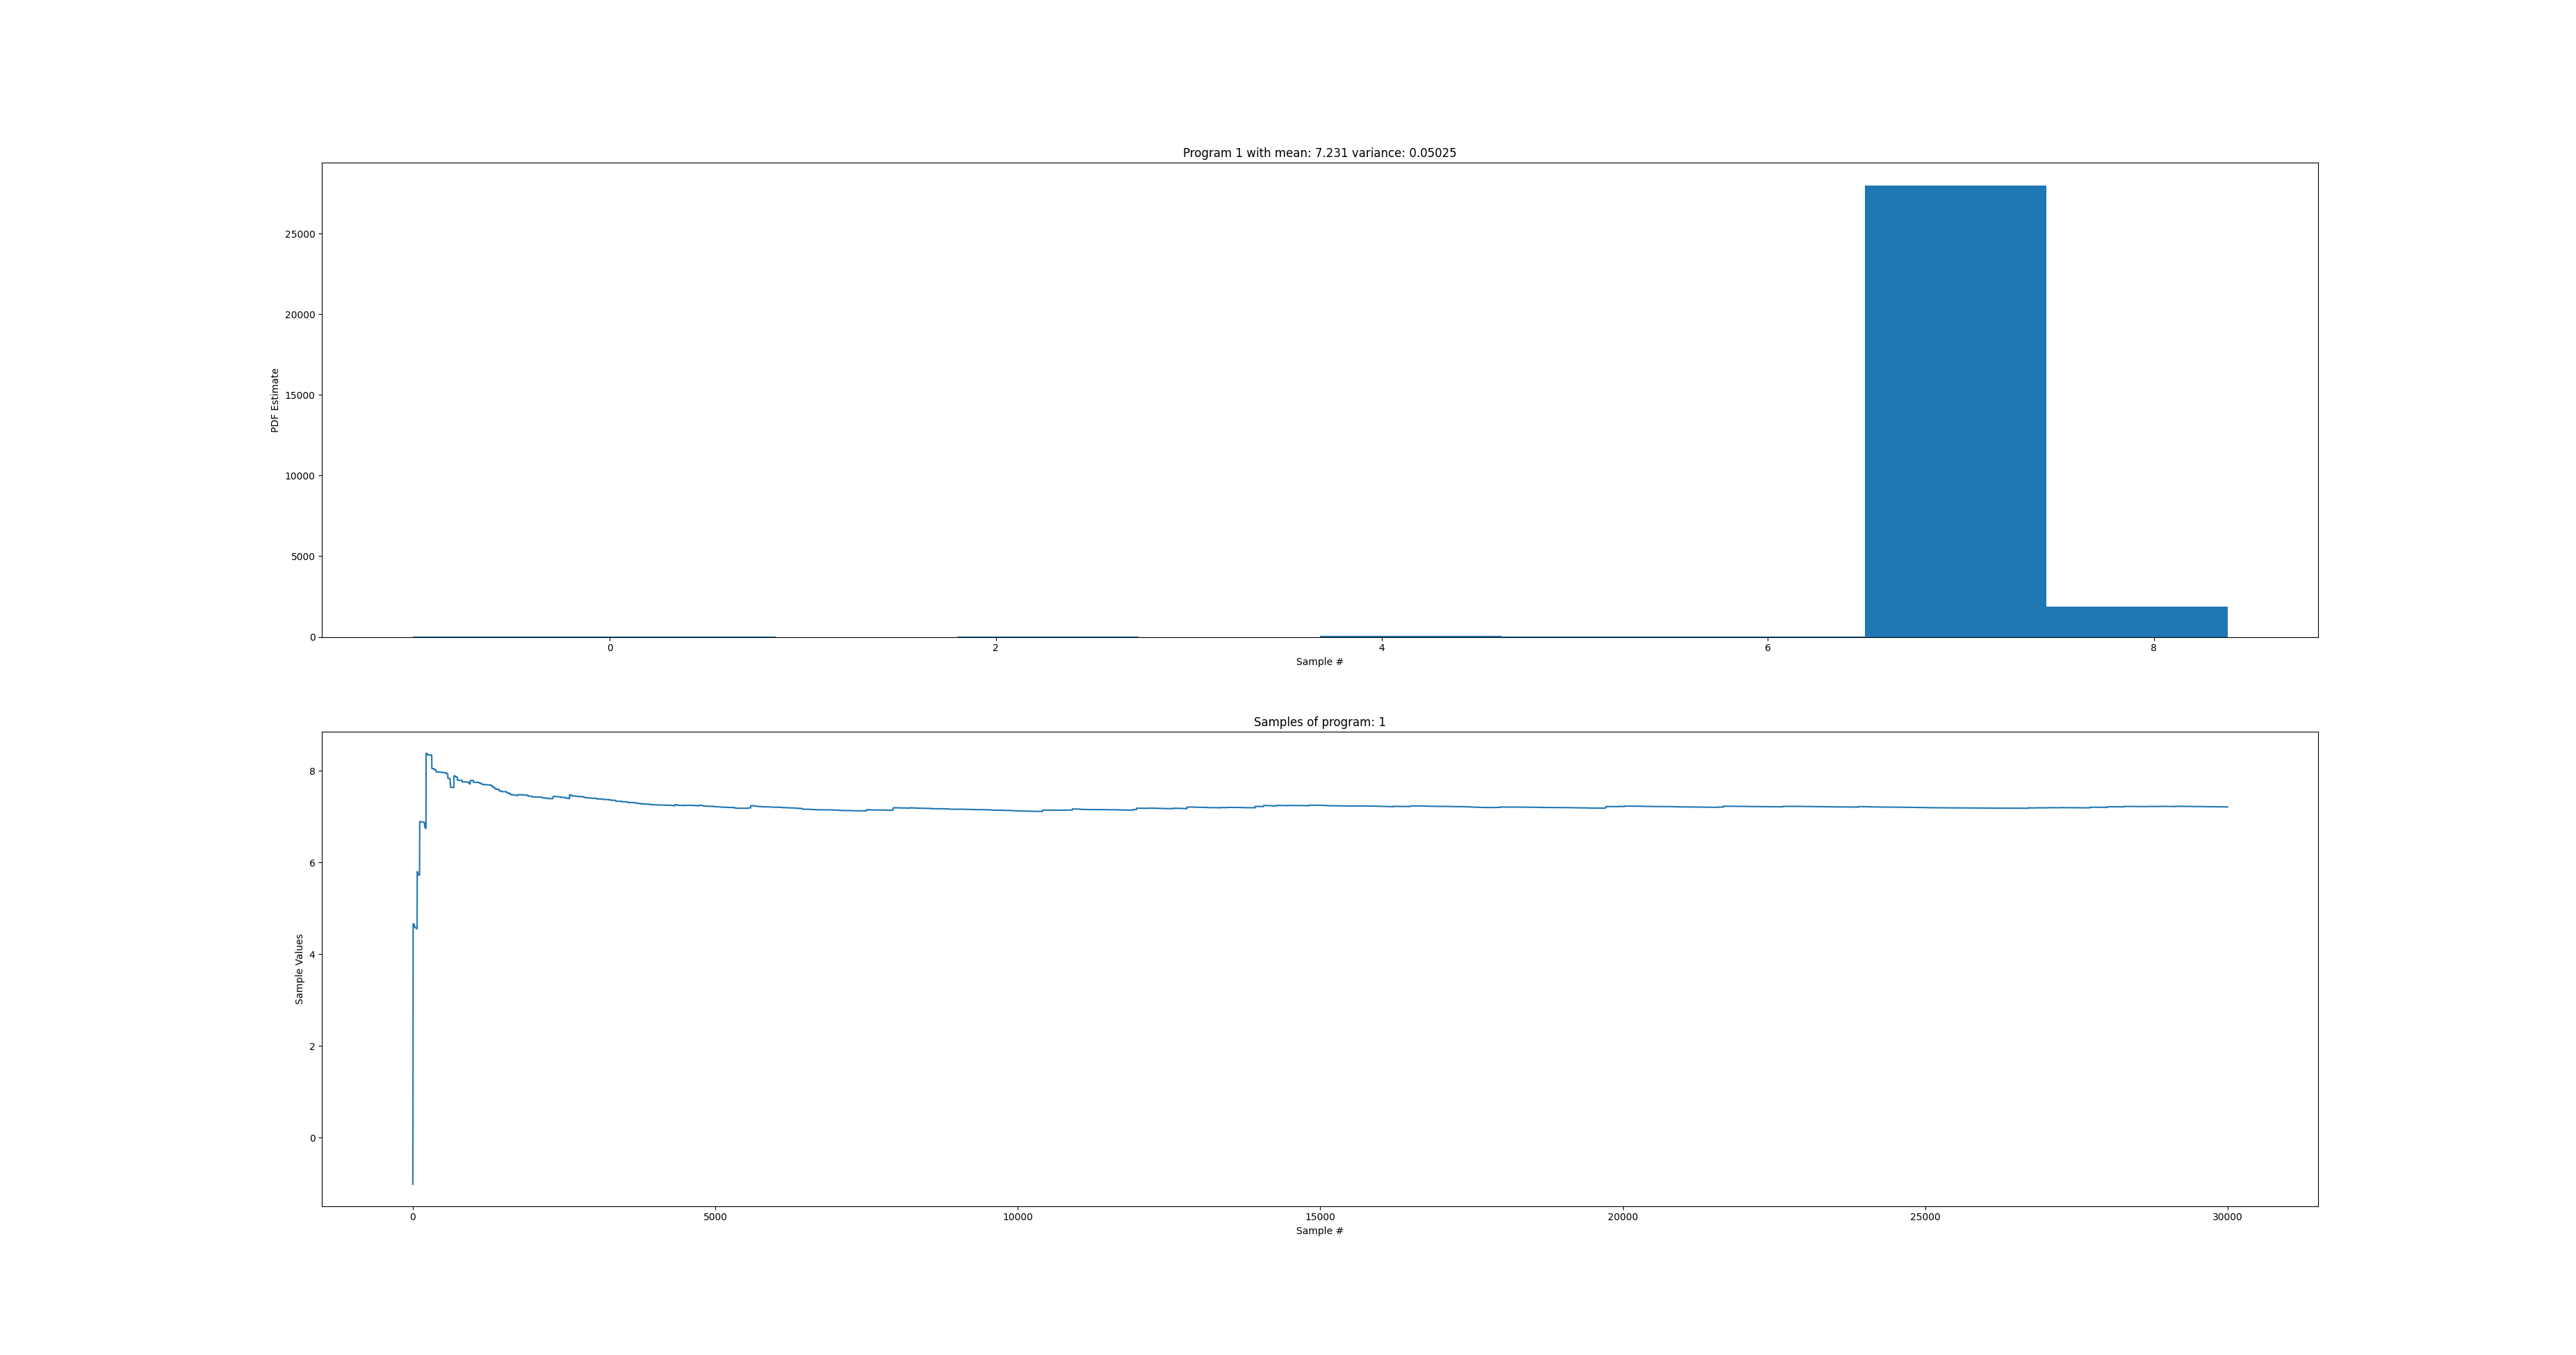
\includegraphics[width=\linewidth]{Figures/p1_IS.png}
\end{center}
\begin{center}
	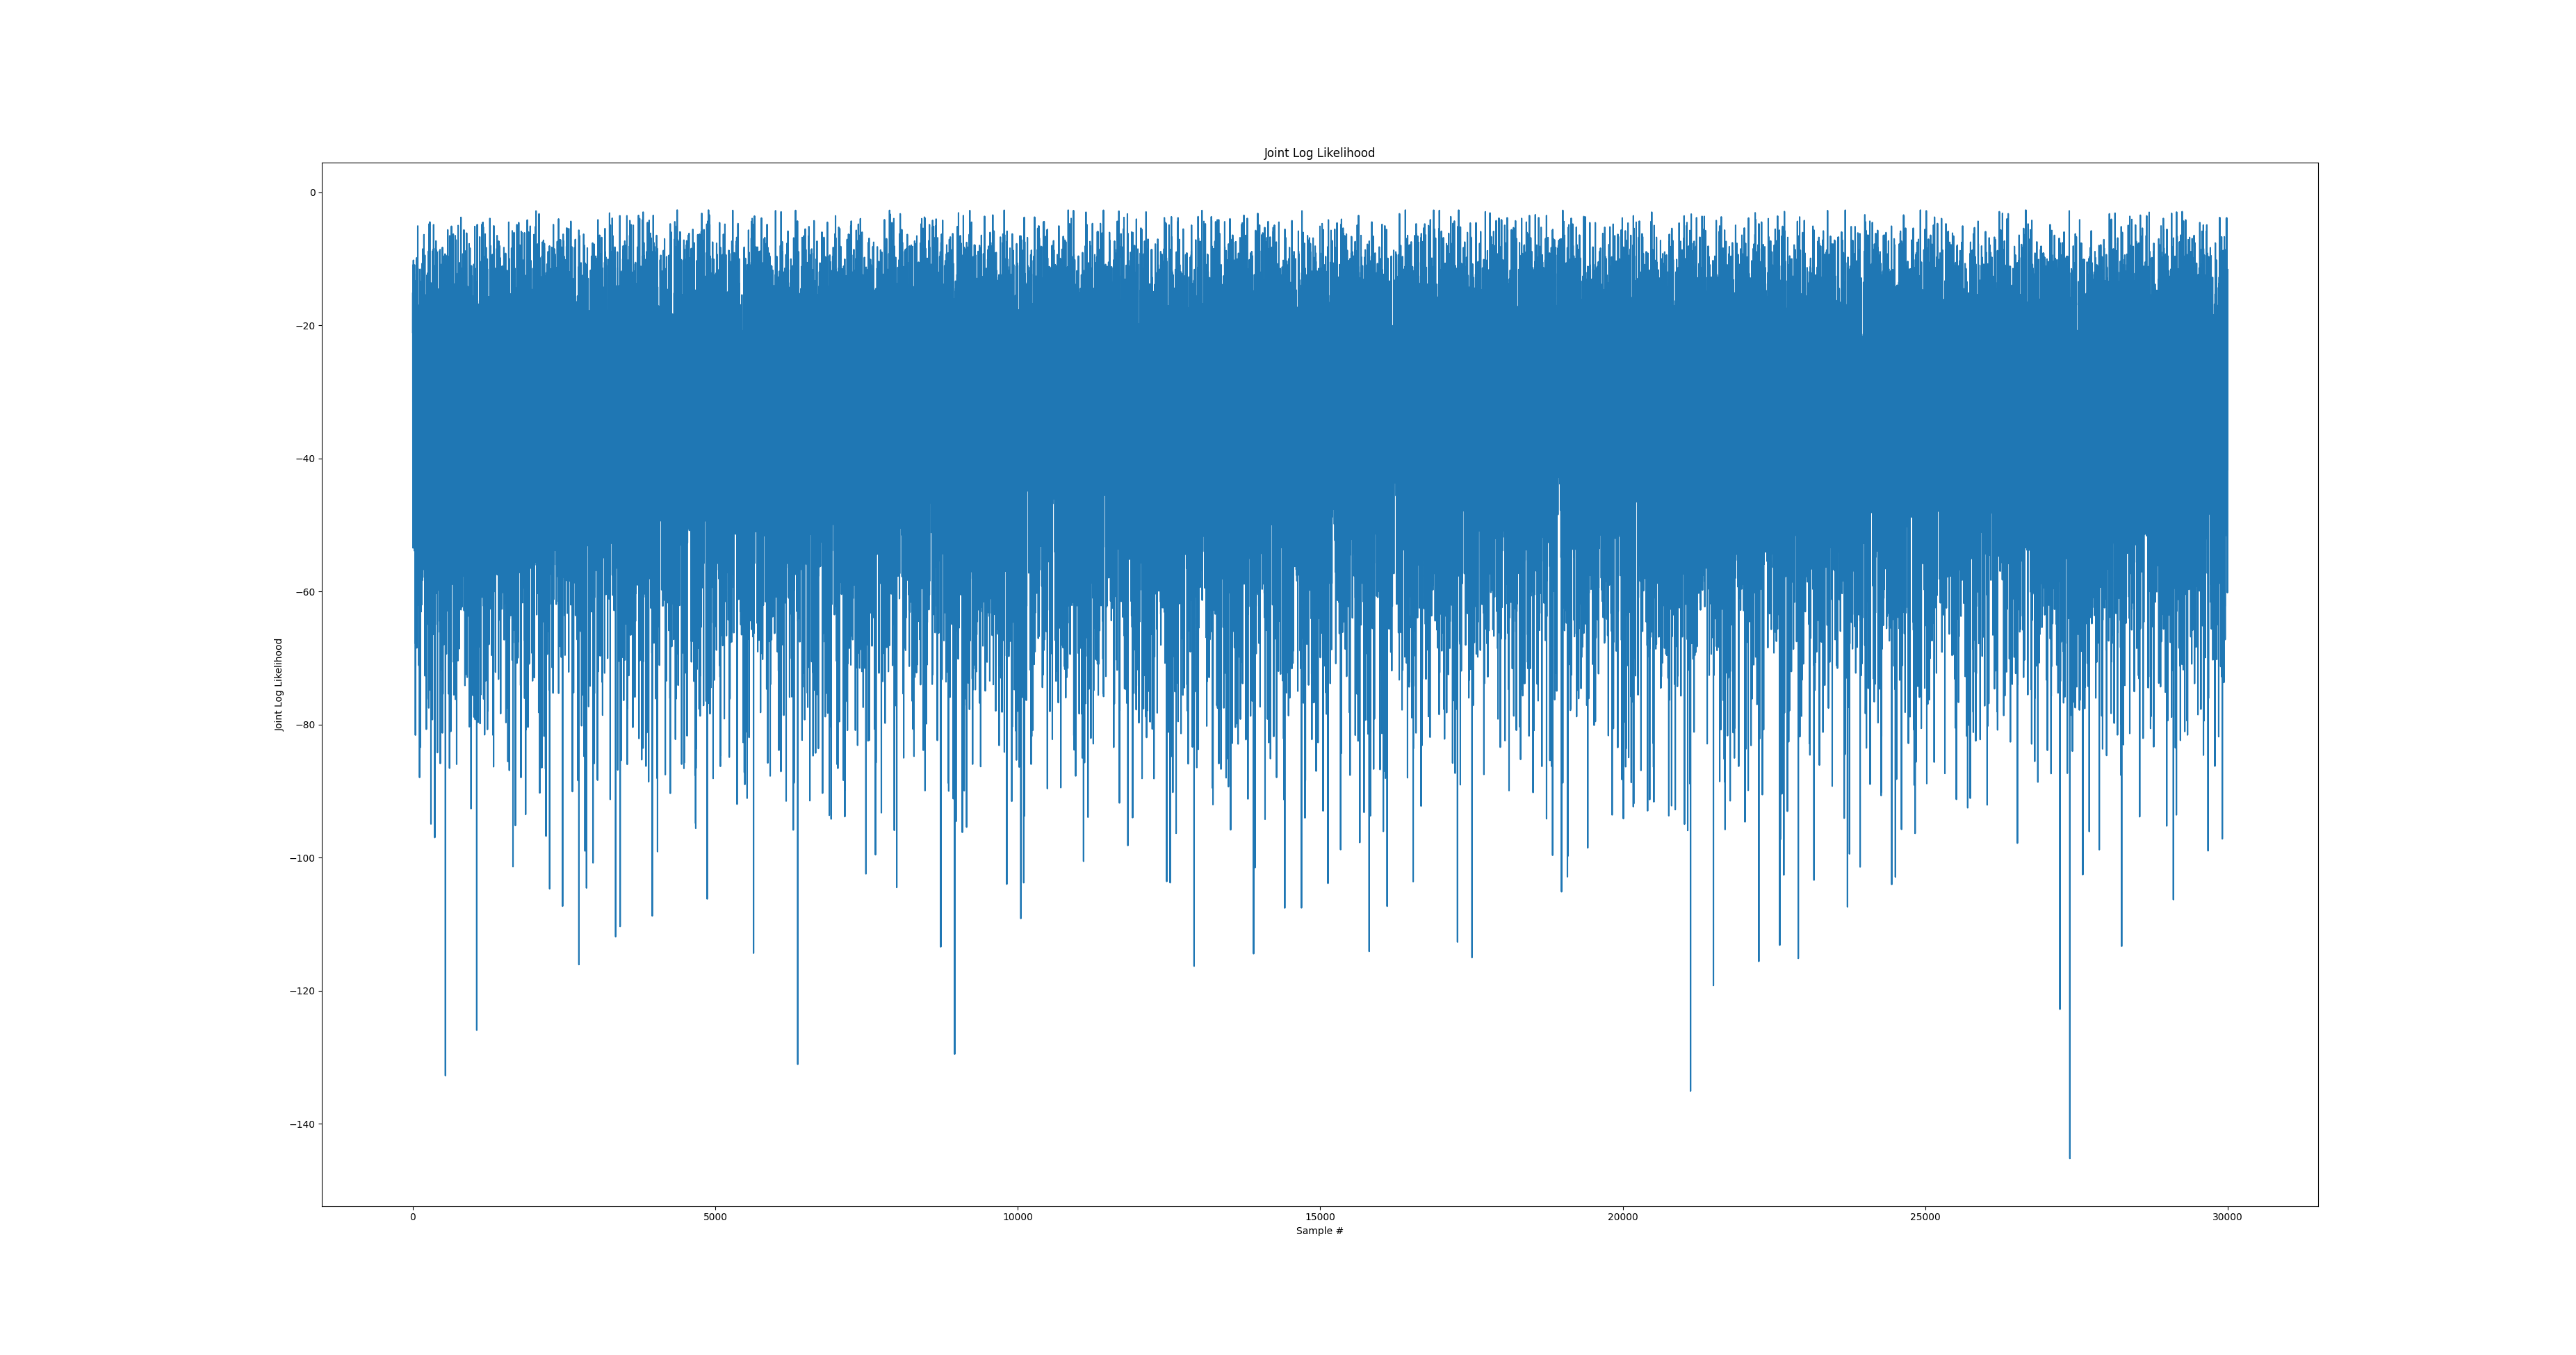
\includegraphics[width=\linewidth]{Figures/p1_ISjll.png}
\end{center}
\subsection{Program 2}
\begin{verbatim}
Collect samples denoted by program 2:
Elapsed time for program  2 .daphne is:  0:00:50.207221  seconds
tensor([ 2.1535, -0.5521])
tensor([[ 4.5837, -7.1774],
[ 4.5837, -7.1774],
[ 4.5837, -7.1774],
...,
[ 2.1535, -0.5521],
[ 2.1535, -0.5521],
[ 2.1535, -0.5521]])
Mean of trace:  tensor([ 2.1645, -0.6133])  
and variance of trace:  tensor([0.0069, 0.0998])
The covariance matrix:  
[[ 0.00687998 -0.02219416]
[-0.02219416  0.09982455]]
\end{verbatim}
\begin{center}
	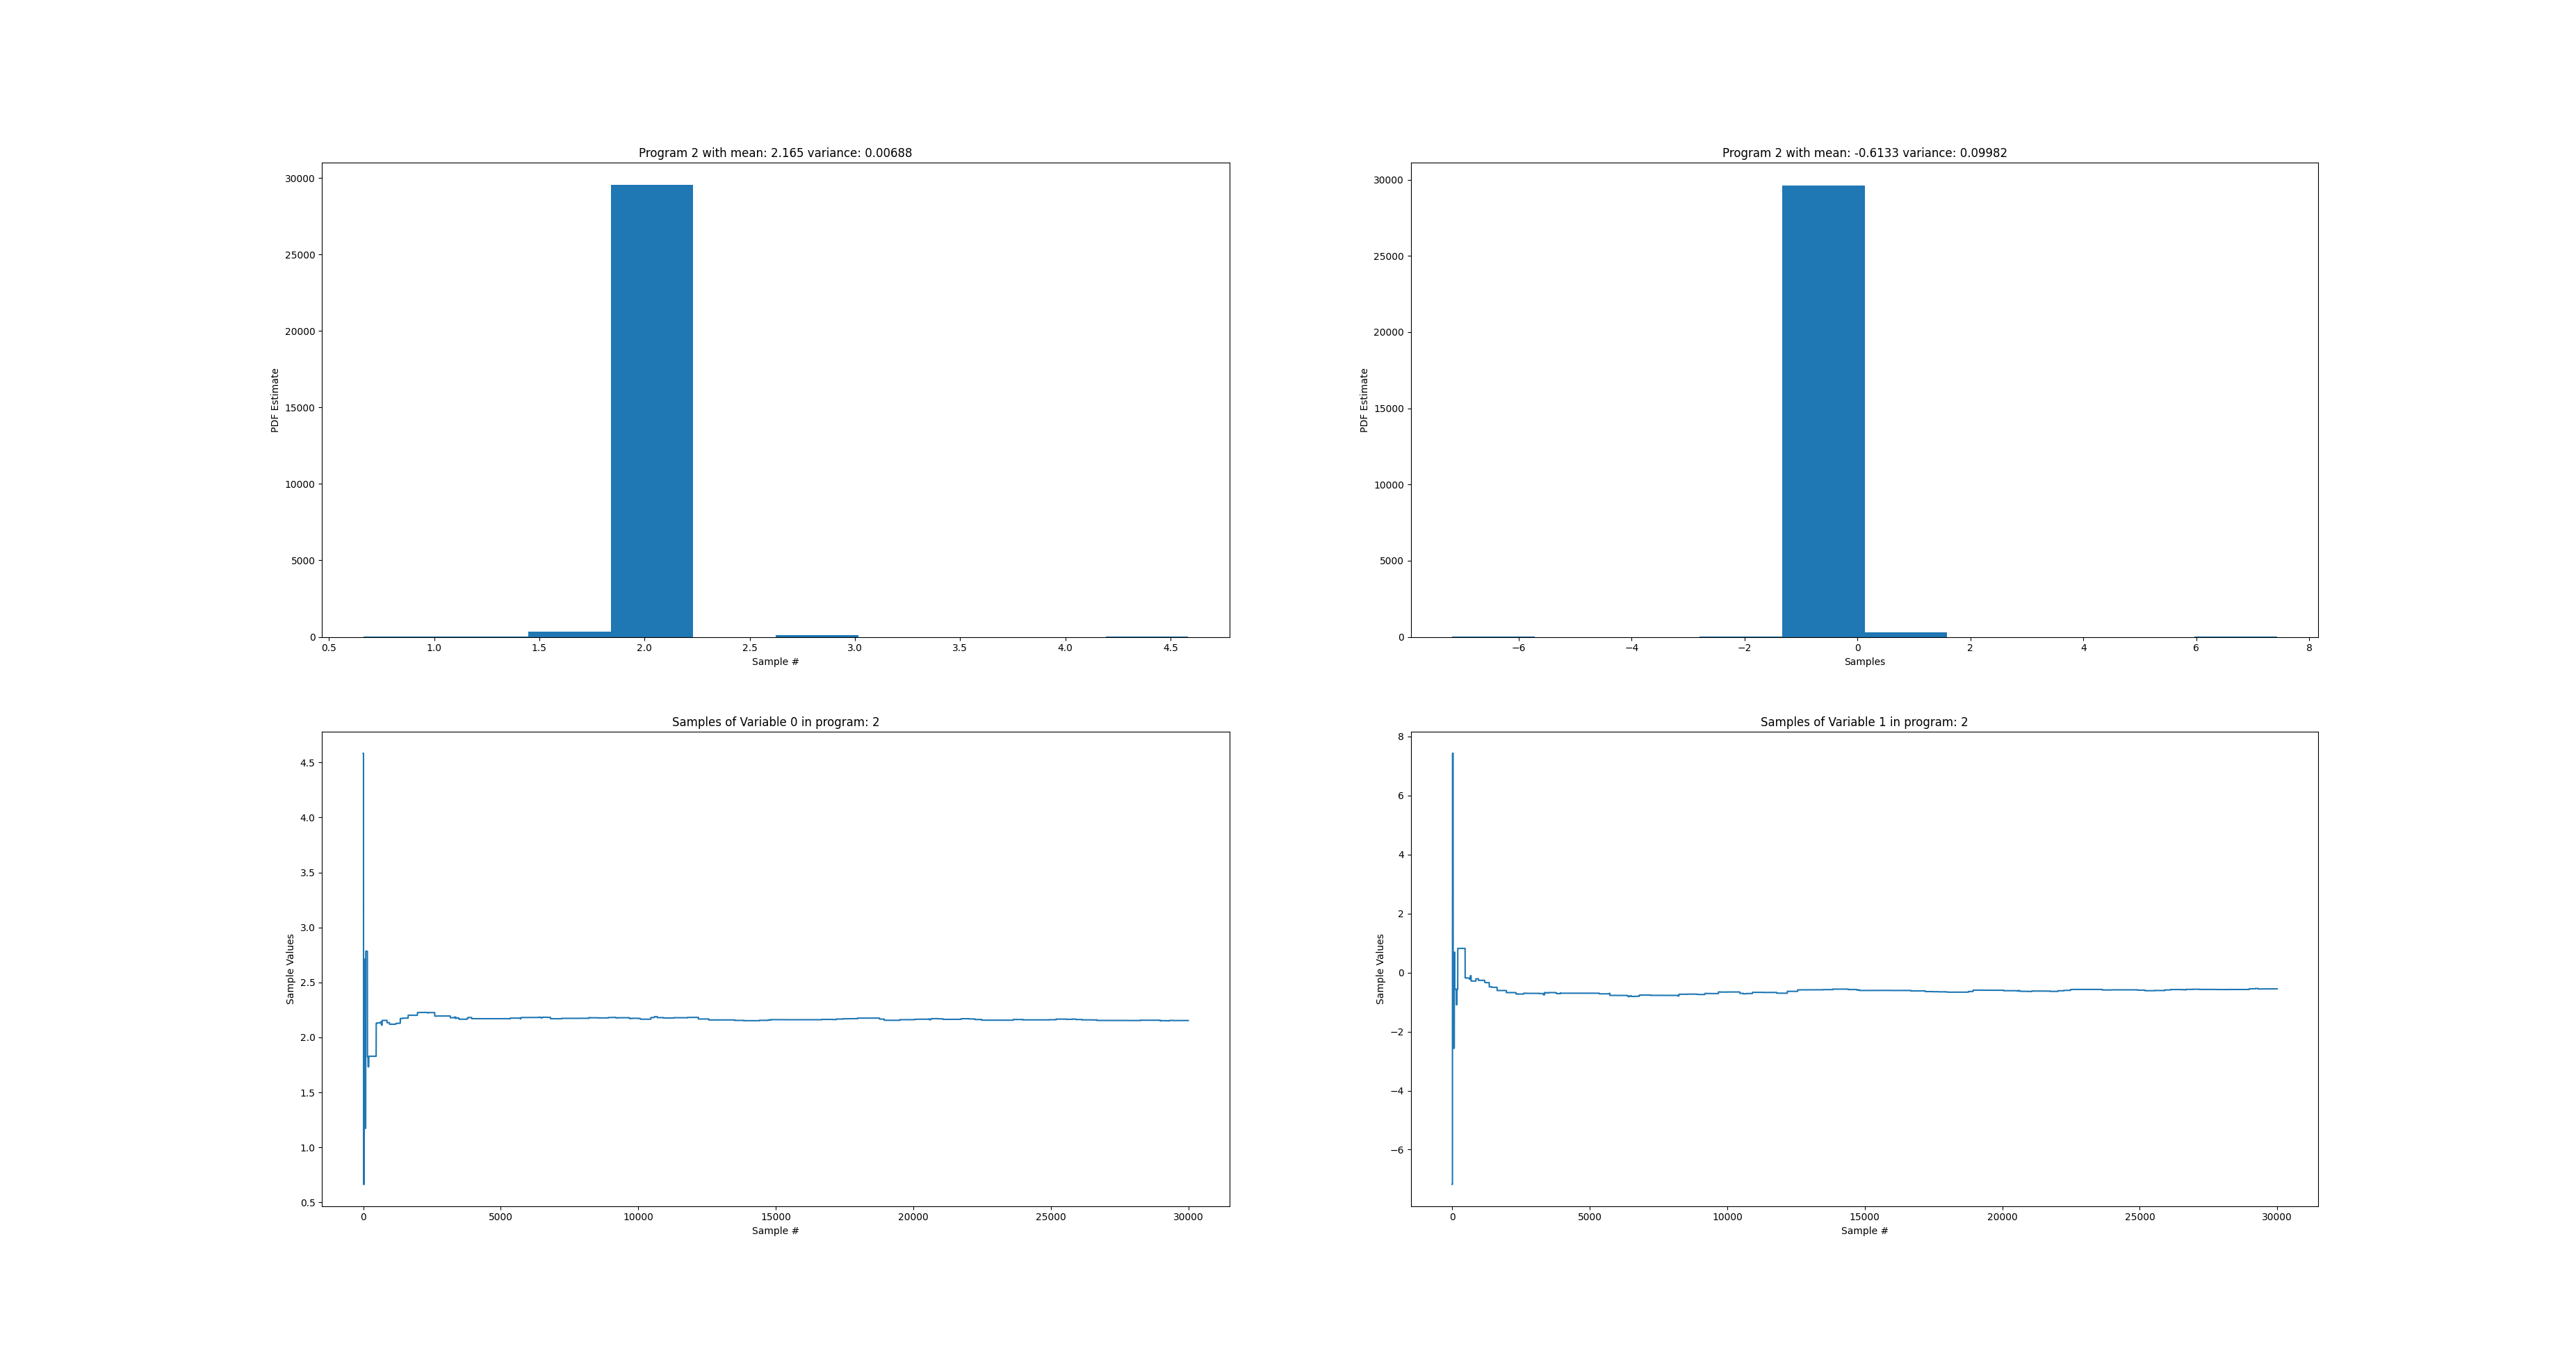
\includegraphics[width=\linewidth]{Figures/p2_IS.png}
\end{center}
\begin{center}
	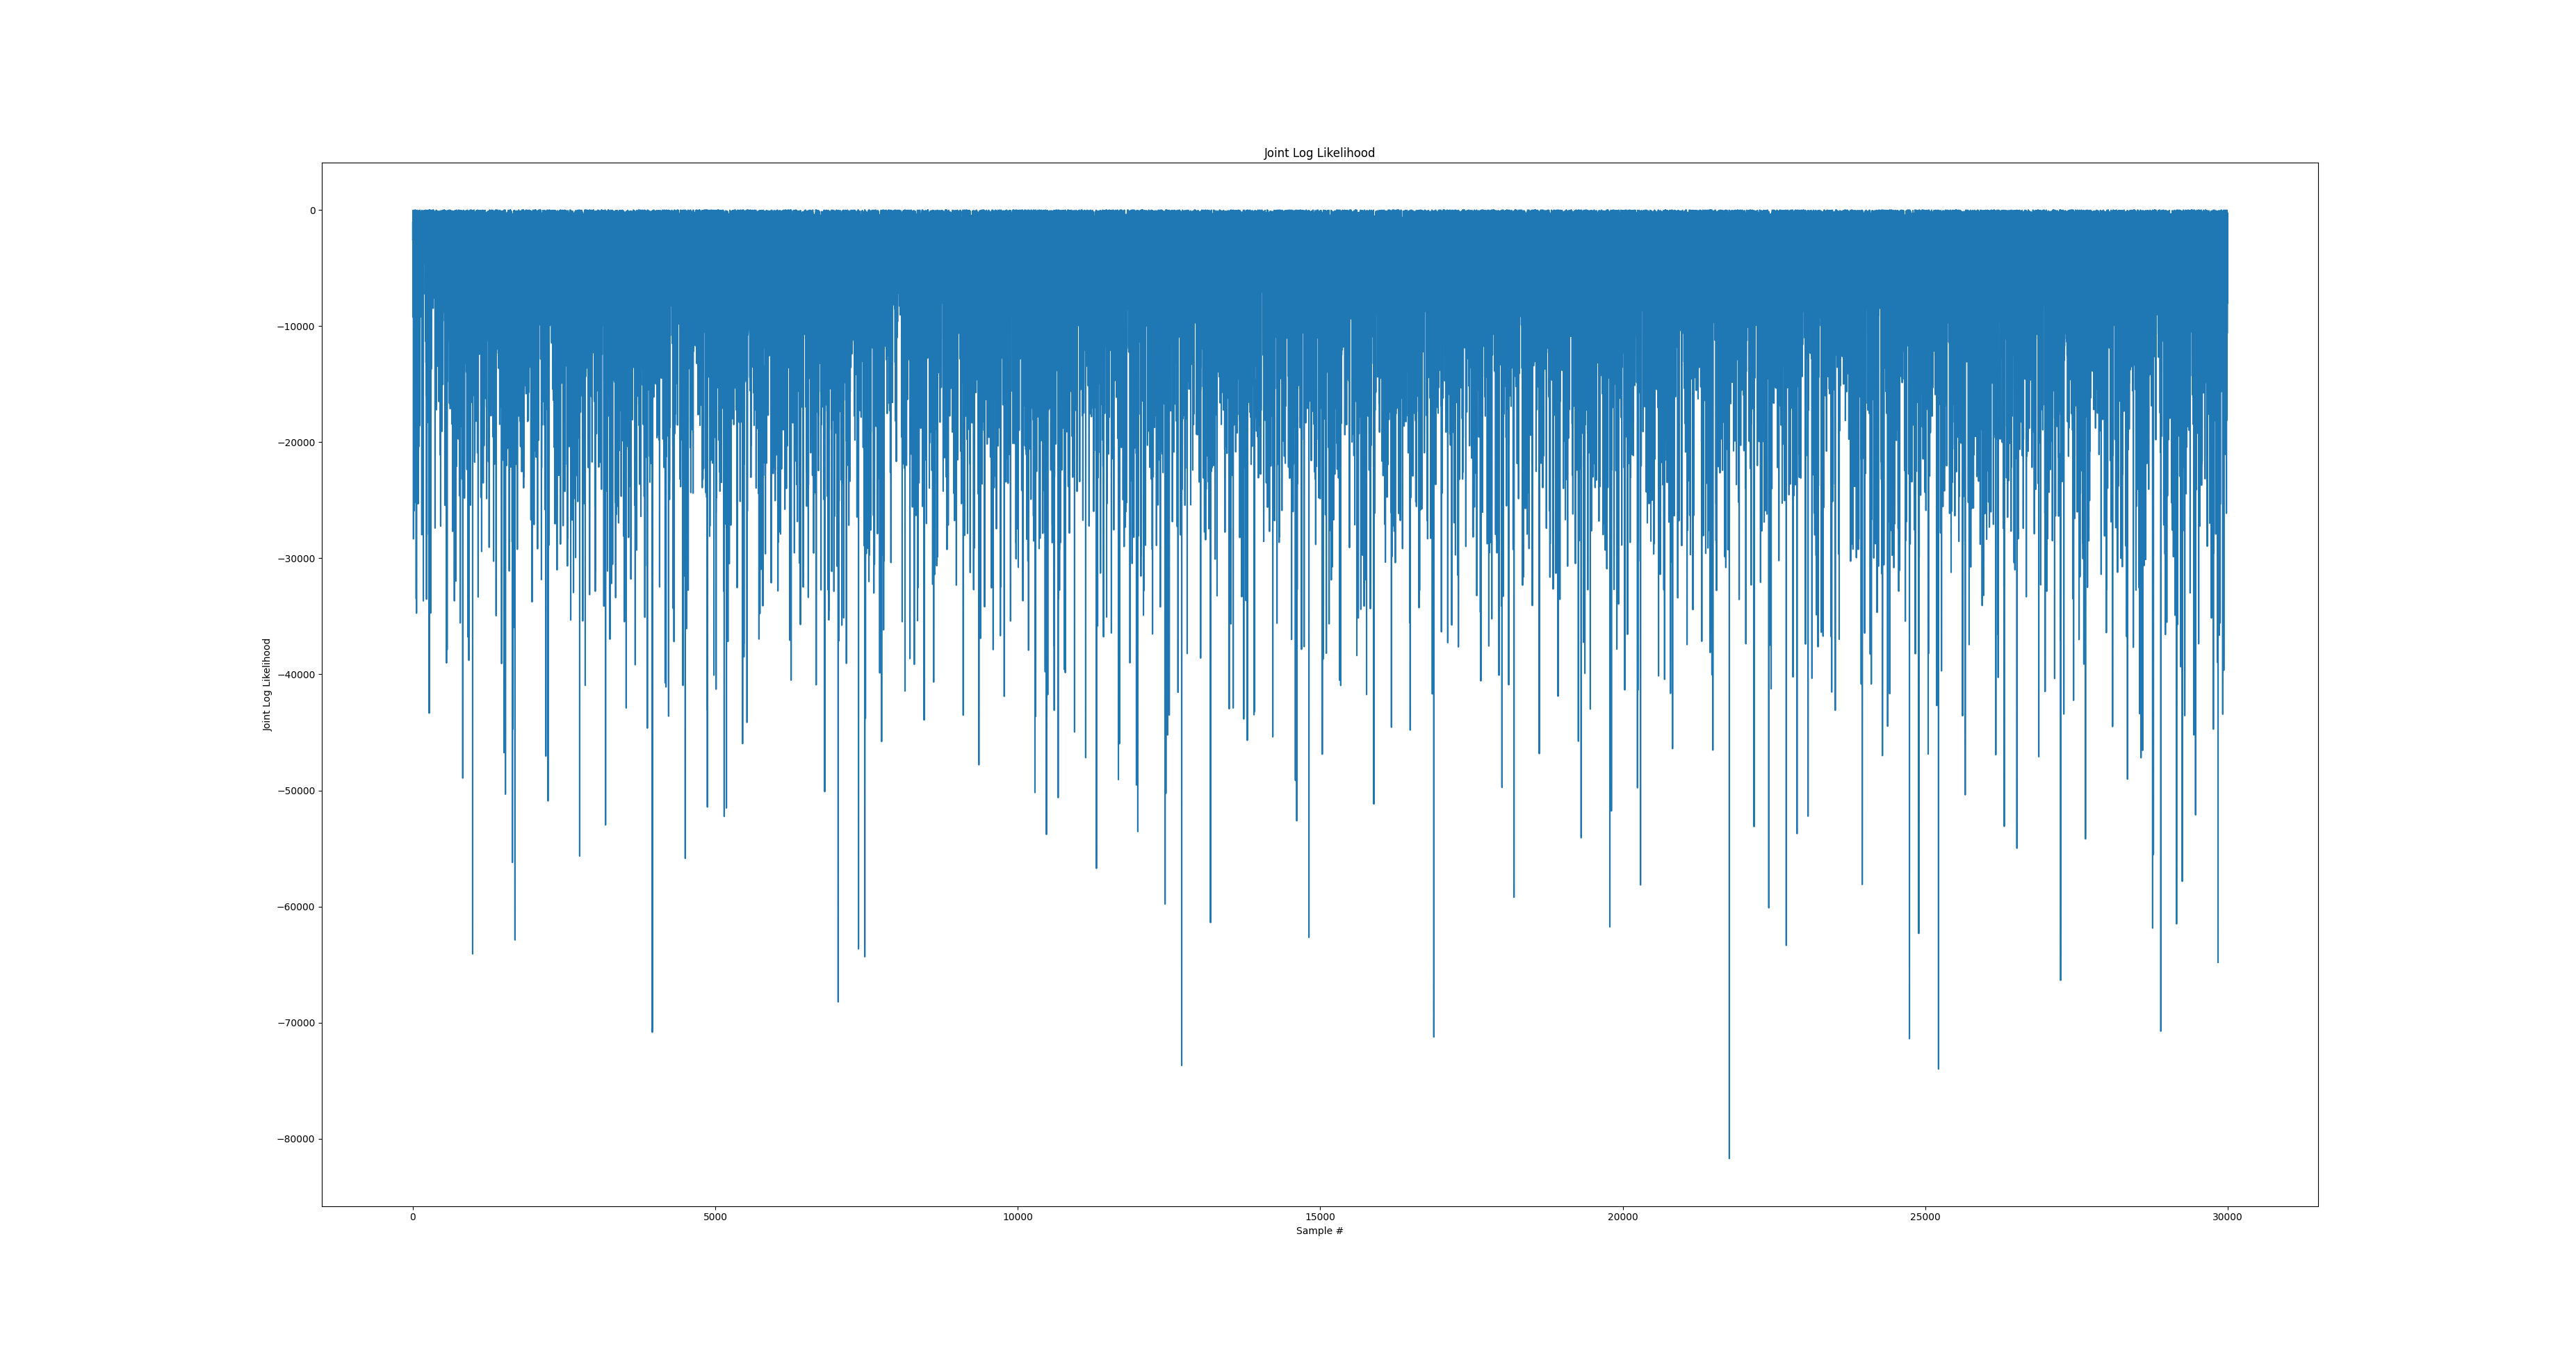
\includegraphics[width=\linewidth]{Figures/p2_ISjll.png}
\end{center}
\subsection{Program 3}
\begin{verbatim}
Collect samples denoted by program 3:
Elapsed time for program  3 .daphne is:  0:00:59.699769  seconds
tensor(0.6275)
tensor([0.0000, 0.0000, 0.4917,  ..., 0.6275, 0.6275, 0.6275])
Mean of trace:  tensor(0.5551)  
and variance of trace:  tensor(0.0167)
\end{verbatim}
\begin{center}
	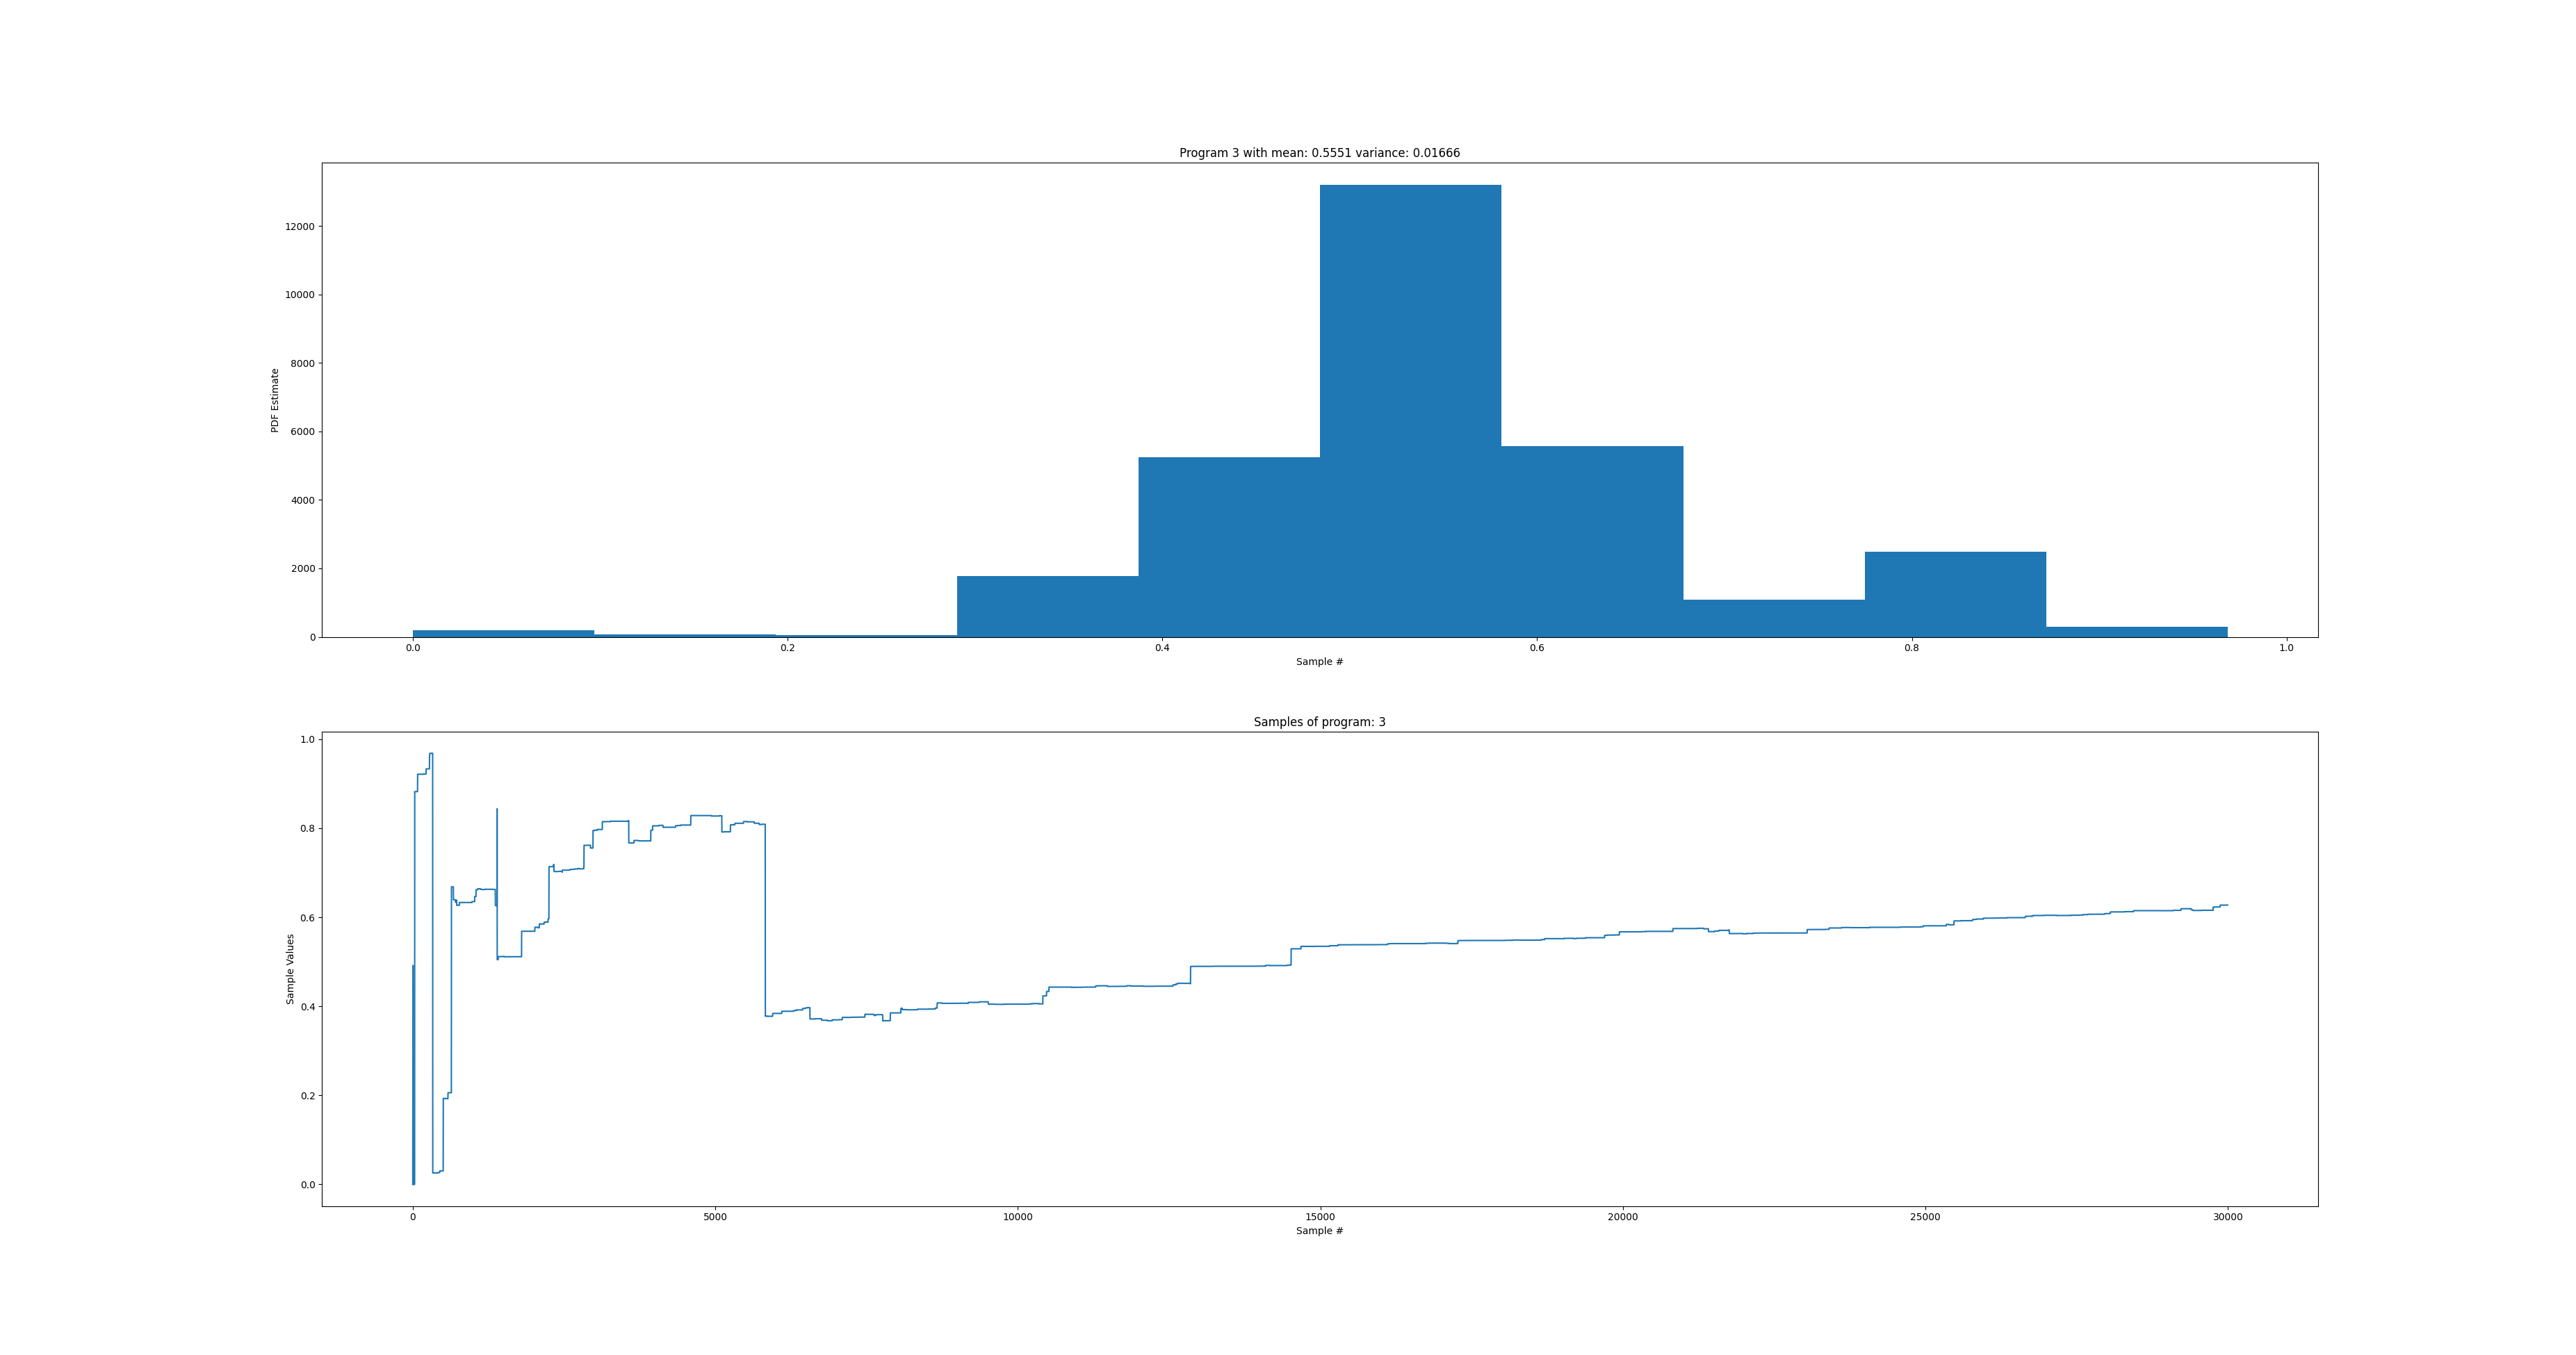
\includegraphics[width=\linewidth]{Figures/p3_IS.png}
\end{center}
\begin{center}
	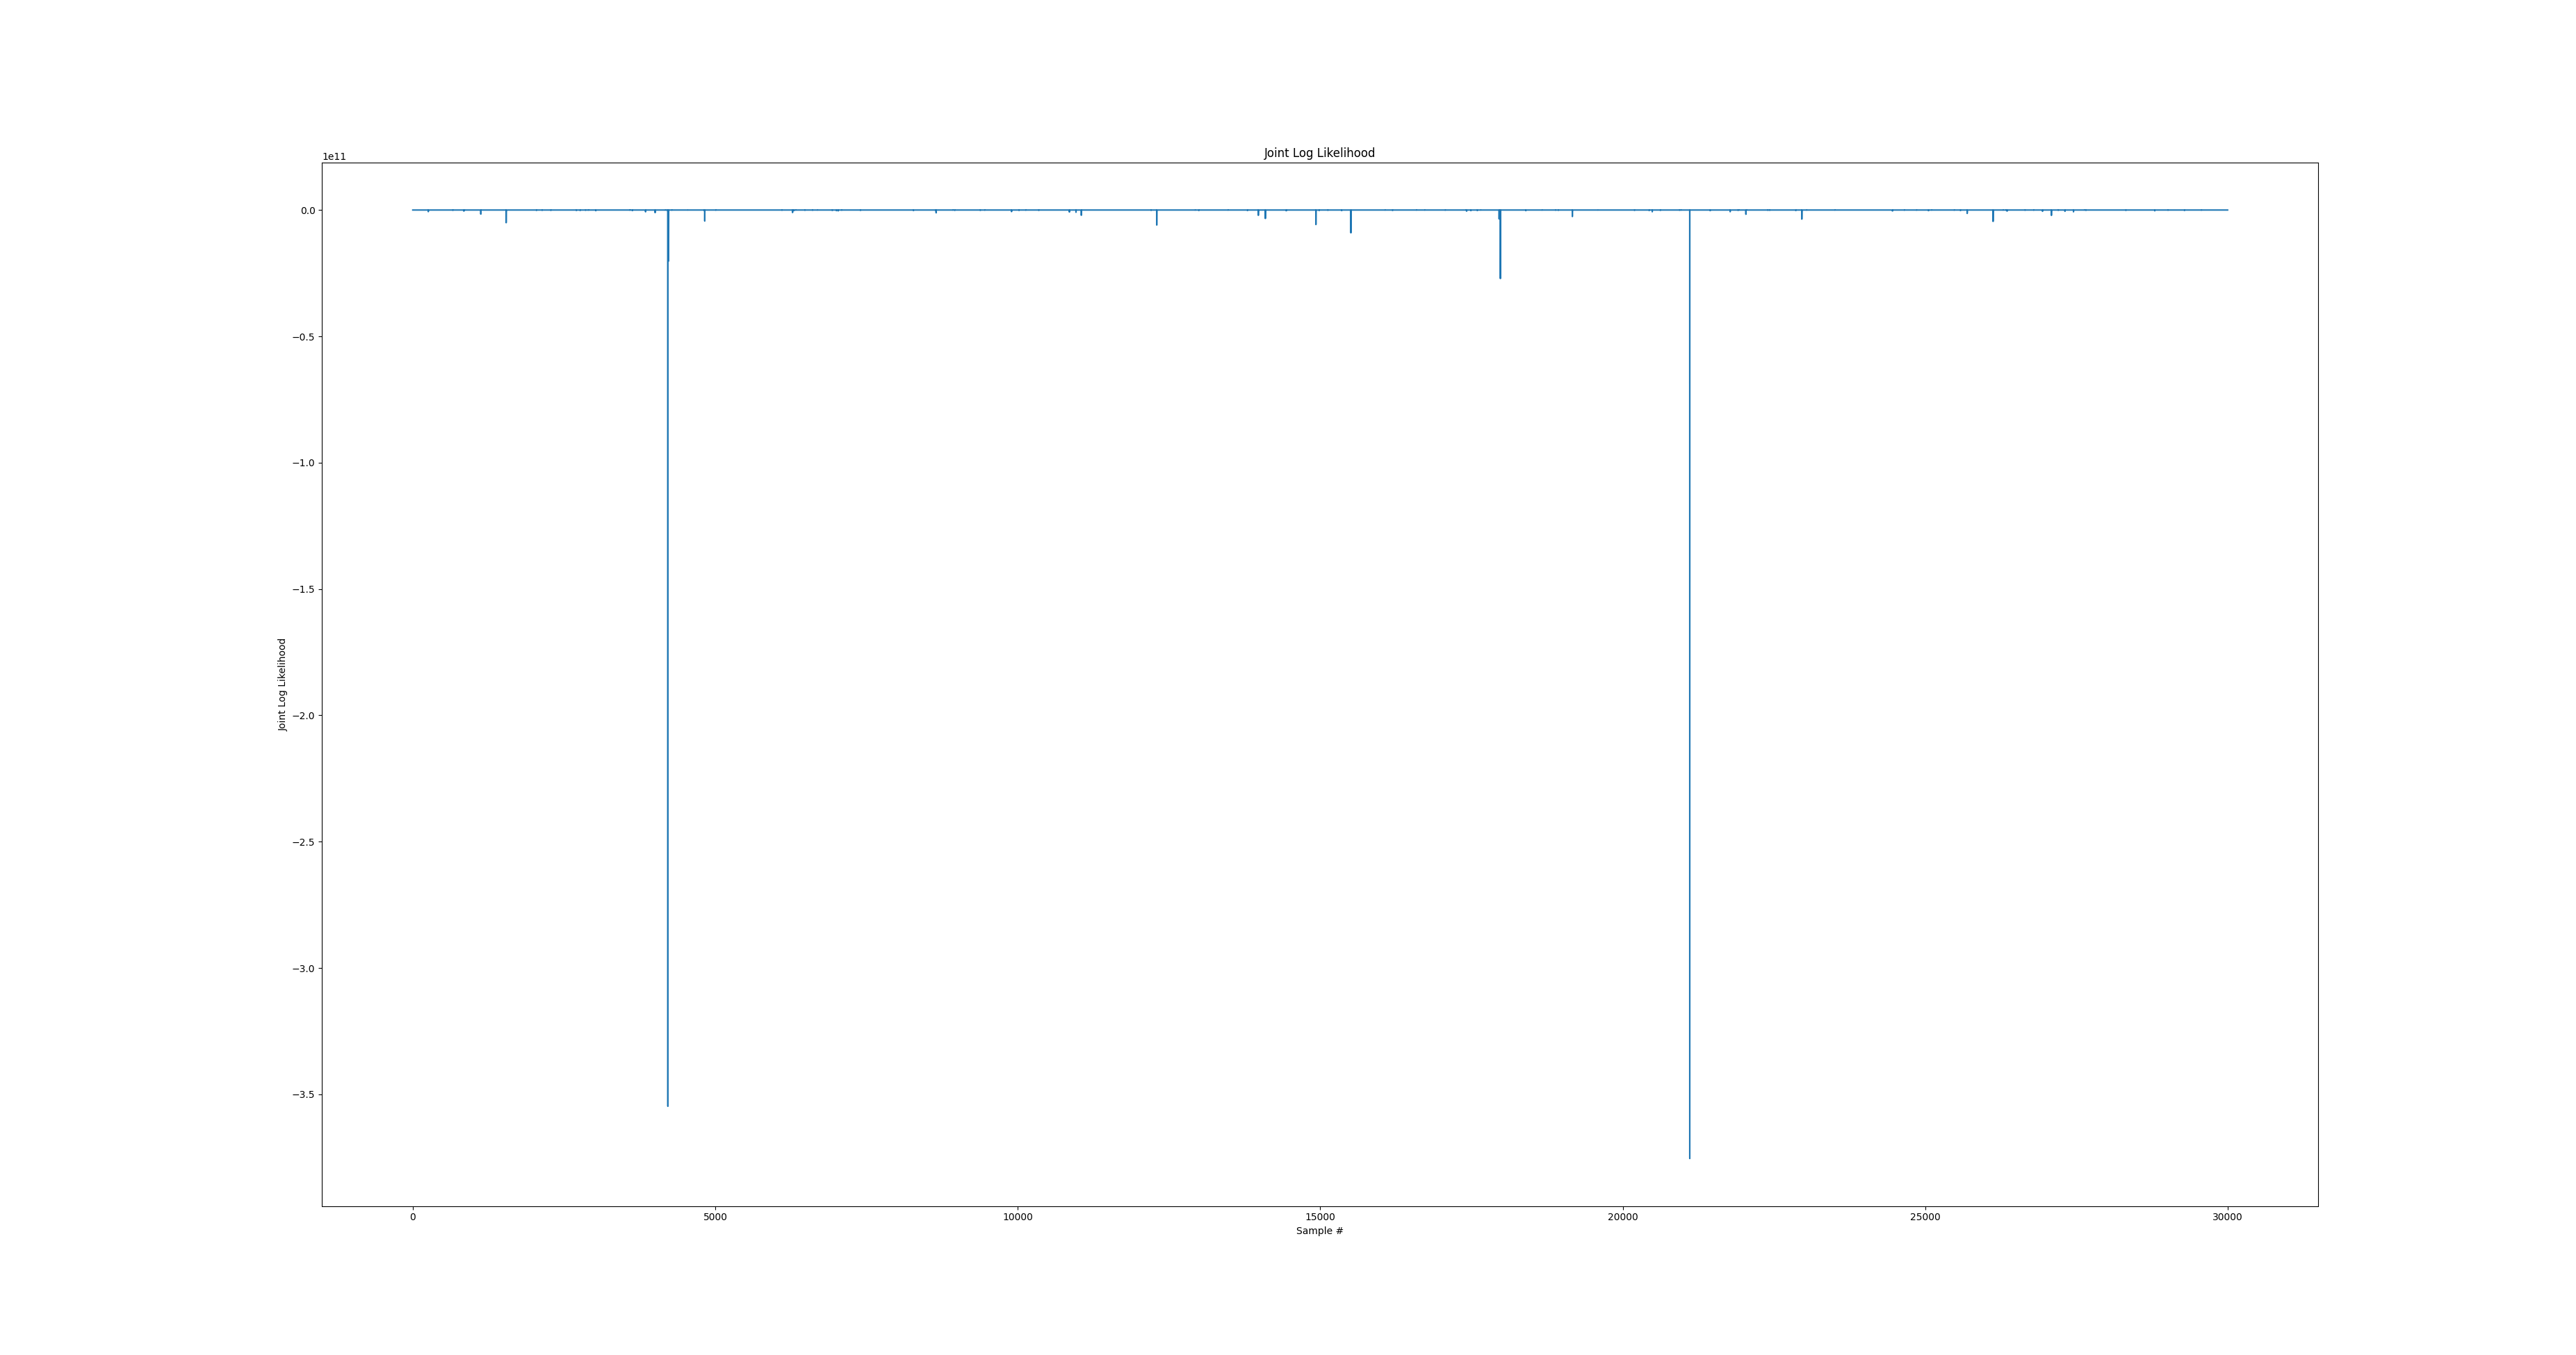
\includegraphics[width=\linewidth]{Figures/p3_ISjll.png}
\end{center}
\subsection{Program 4}
\begin{verbatim}
Collect samples denoted by program 4:
Elapsed time for program  4 .daphne is:  0:00:18.411620  seconds
tensor(0.3158)
tensor([1.0000, 1.0000, 0.5690,  ..., 0.3158, 0.3158, 0.3158])
Mean of trace:  tensor(0.3148)  
and variance of trace:  tensor(0.0001)
\end{verbatim}
\begin{center}
	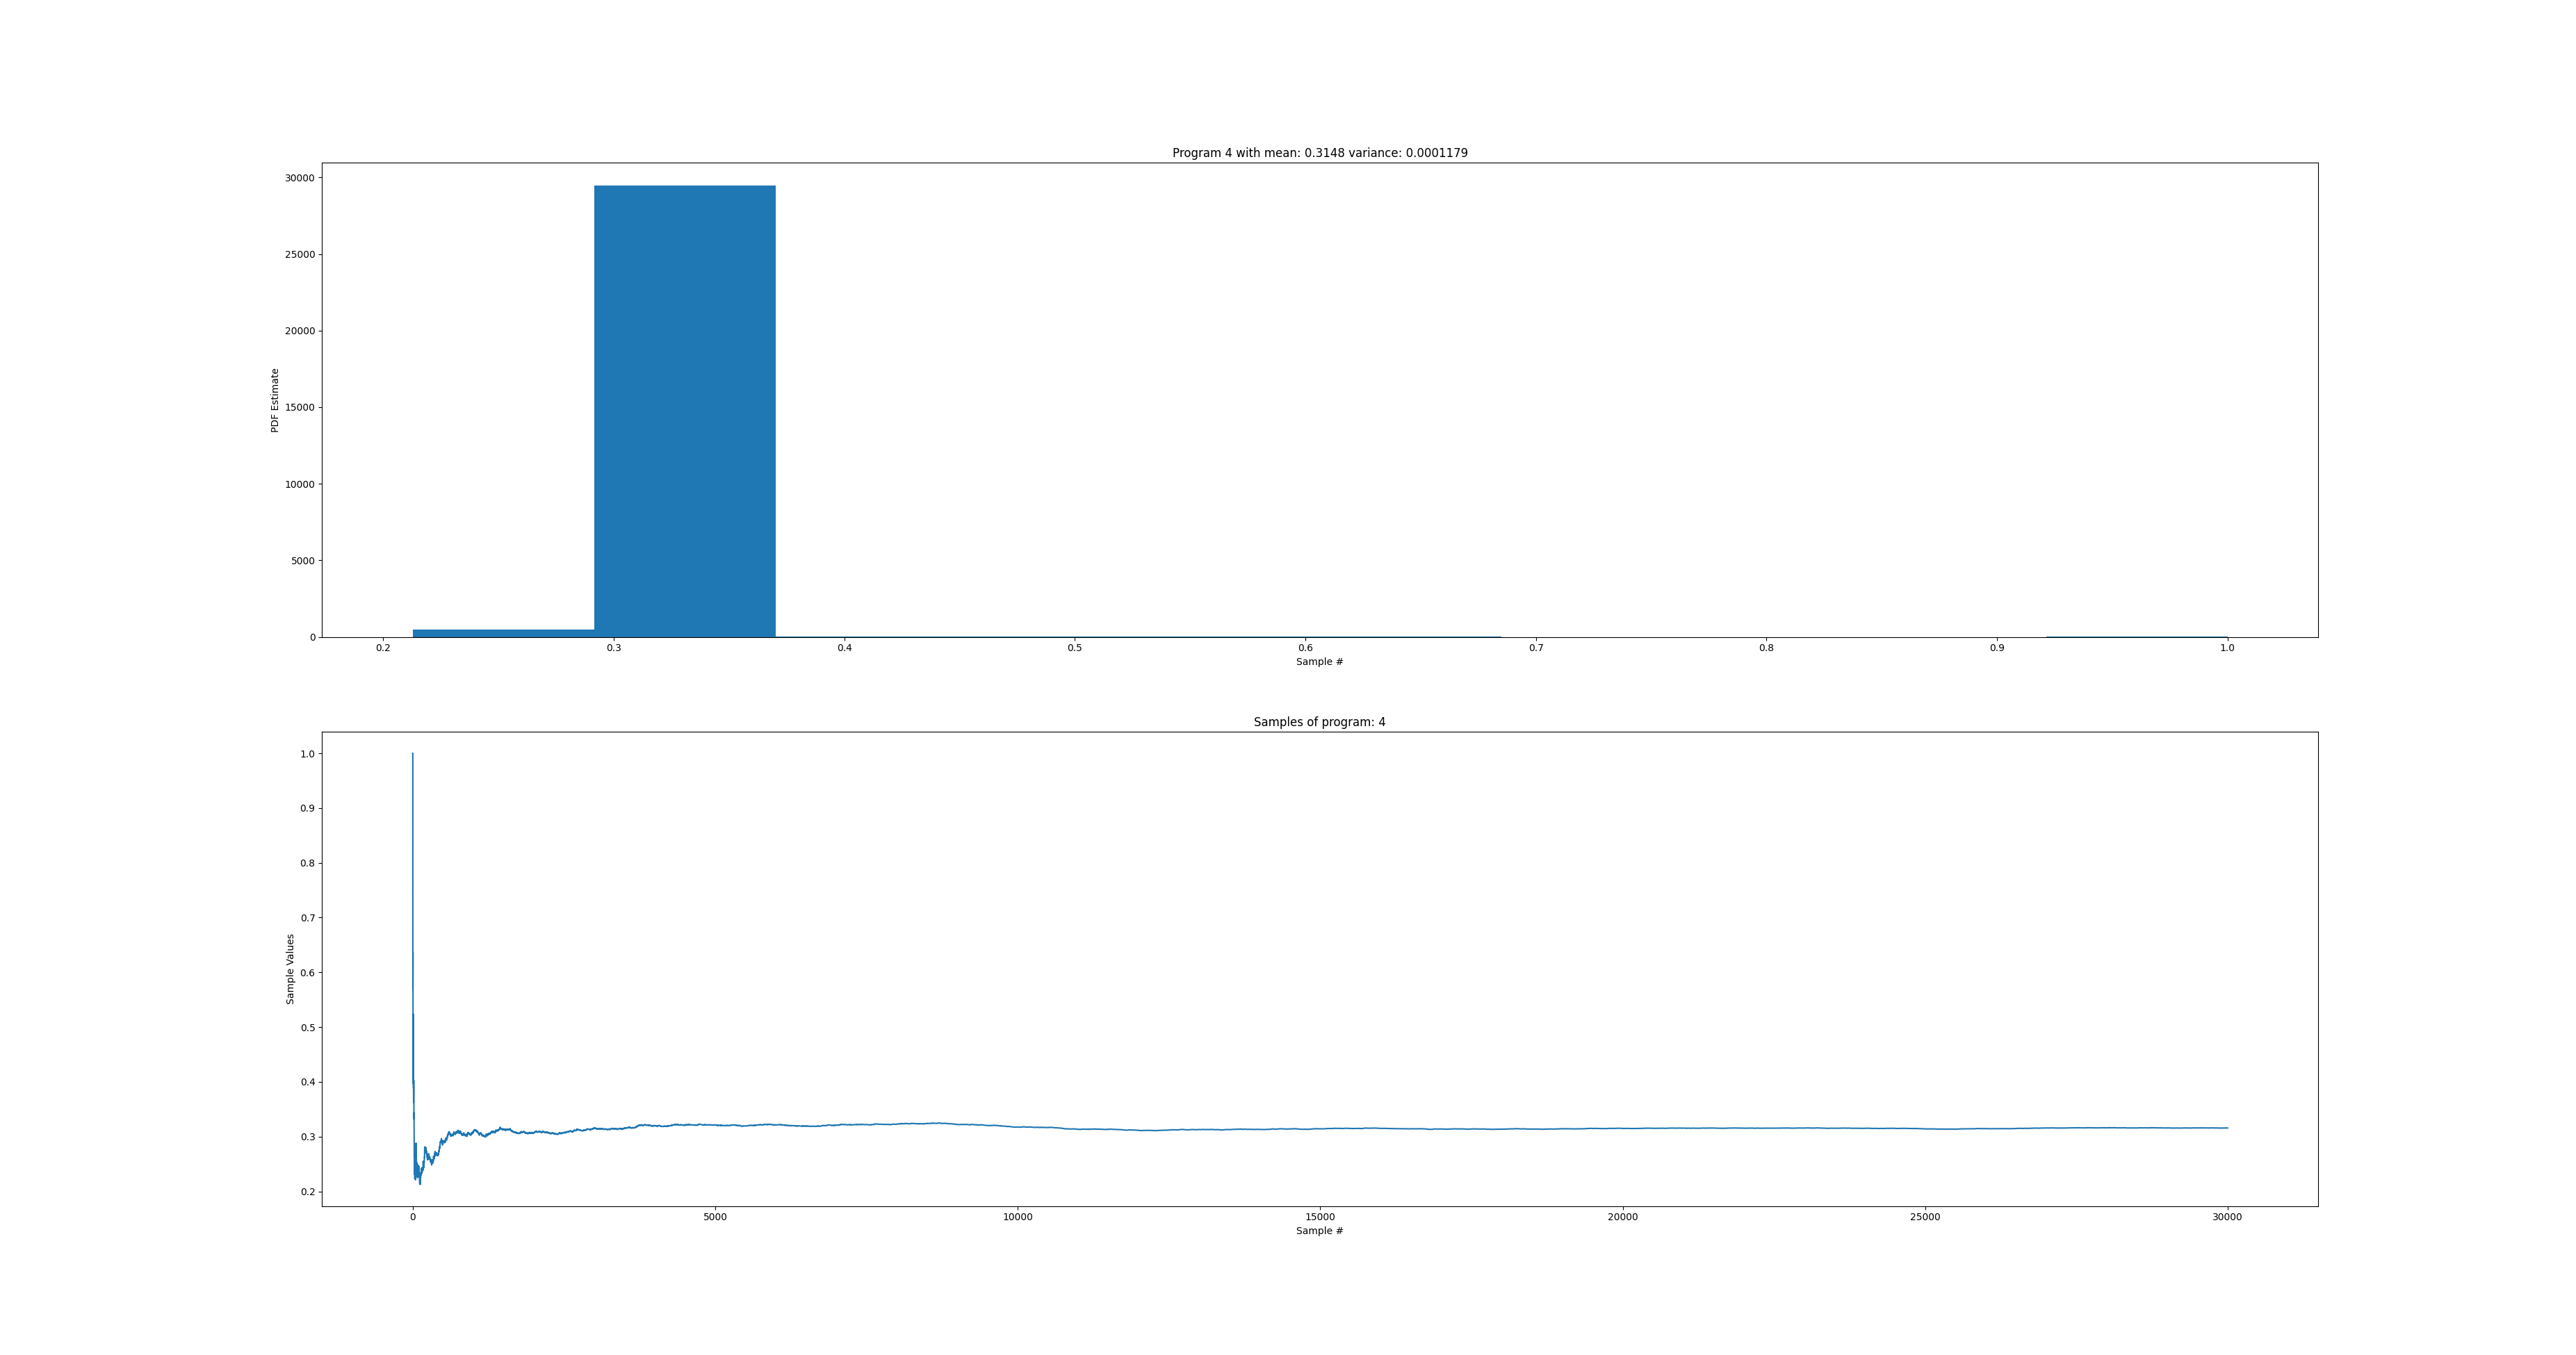
\includegraphics[width=\linewidth]{Figures/p4_IS.png}
\end{center}
\begin{center}
	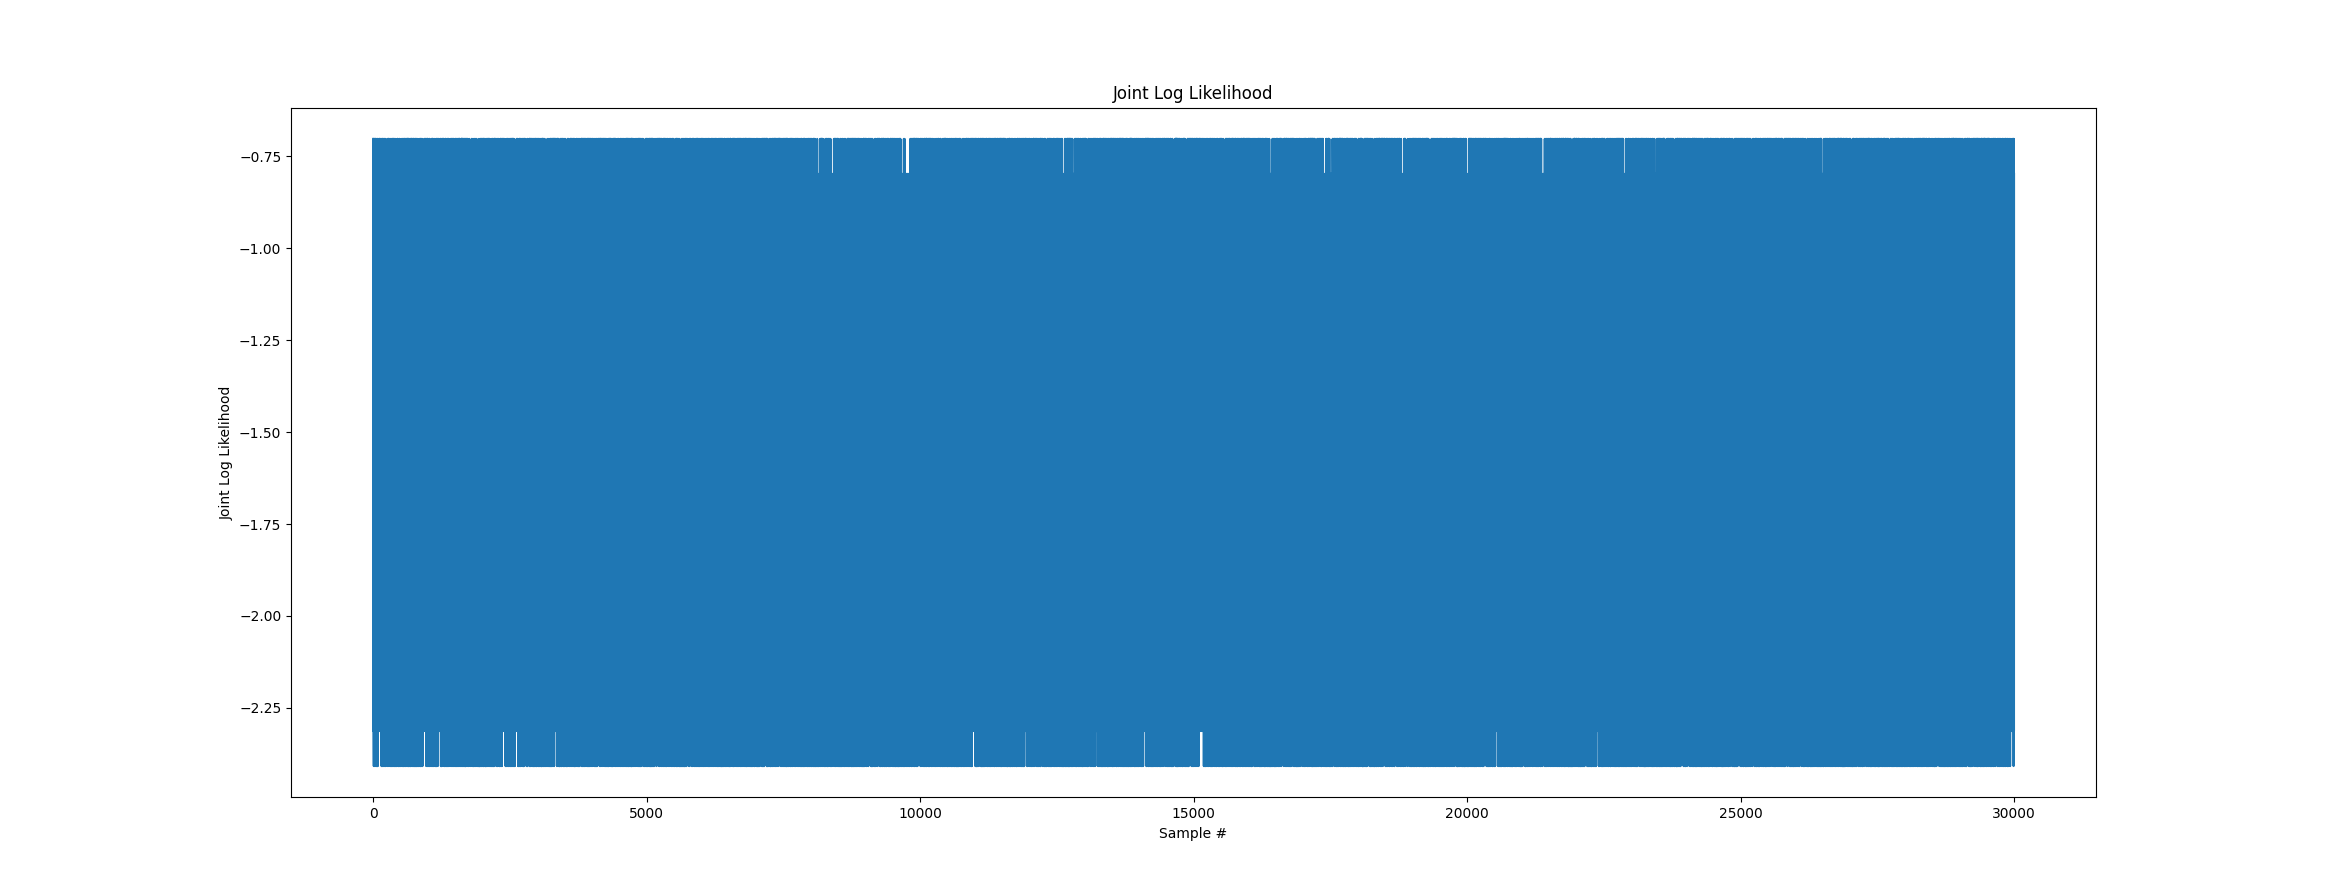
\includegraphics[width=\linewidth]{Figures/p4_ISjll.png}
\end{center}
\subsection{Program 5}
\begin{verbatim}
Collect samples denoted by program 5:
Elapsed time for program  5 .daphne is:  0:00:11.613676  seconds
tensor([2.9748, 4.0338])
tensor([[5.3001, 1.2459],
[5.3001, 1.2459],
[5.3001, 1.2459],
...,
[2.9748, 4.0338],
[2.9748, 4.0338],
[2.9748, 4.0338]])
Mean of trace:  tensor([2.9516, 4.0578])  
and variance of trace:  tensor([0.7594, 0.7662])
\end{verbatim}
\begin{center}
	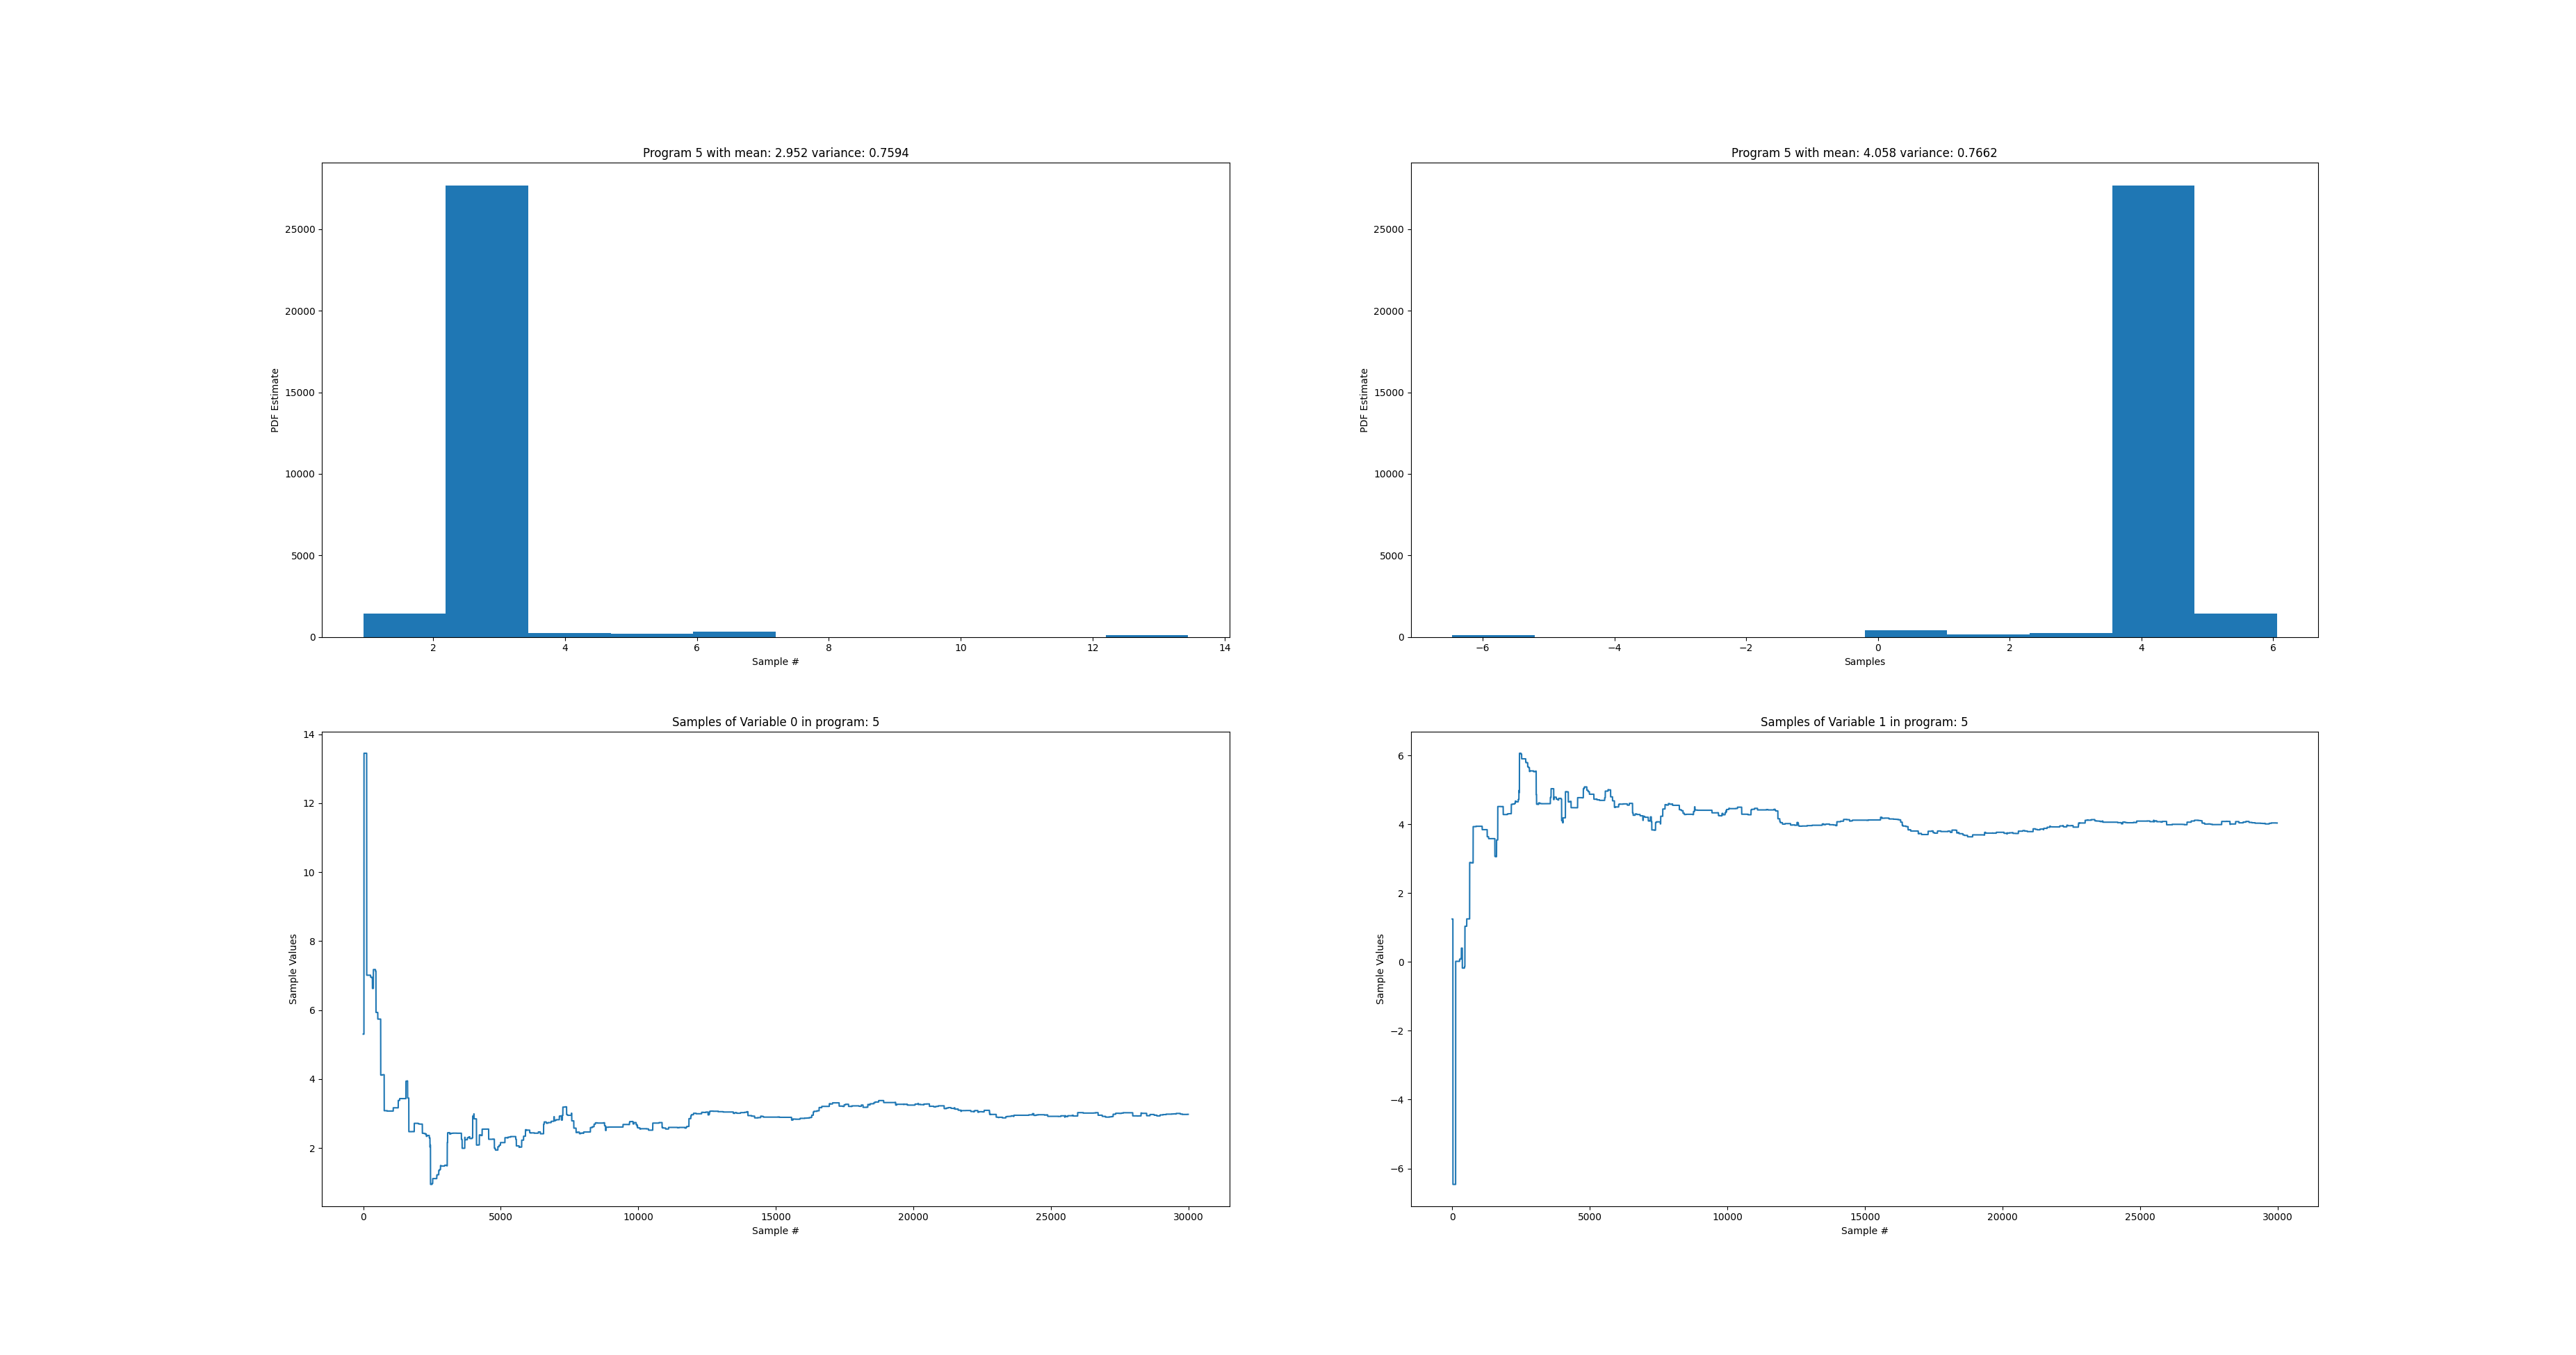
\includegraphics[width=\linewidth]{Figures/p5_IS.png}
\end{center}
\begin{center}
	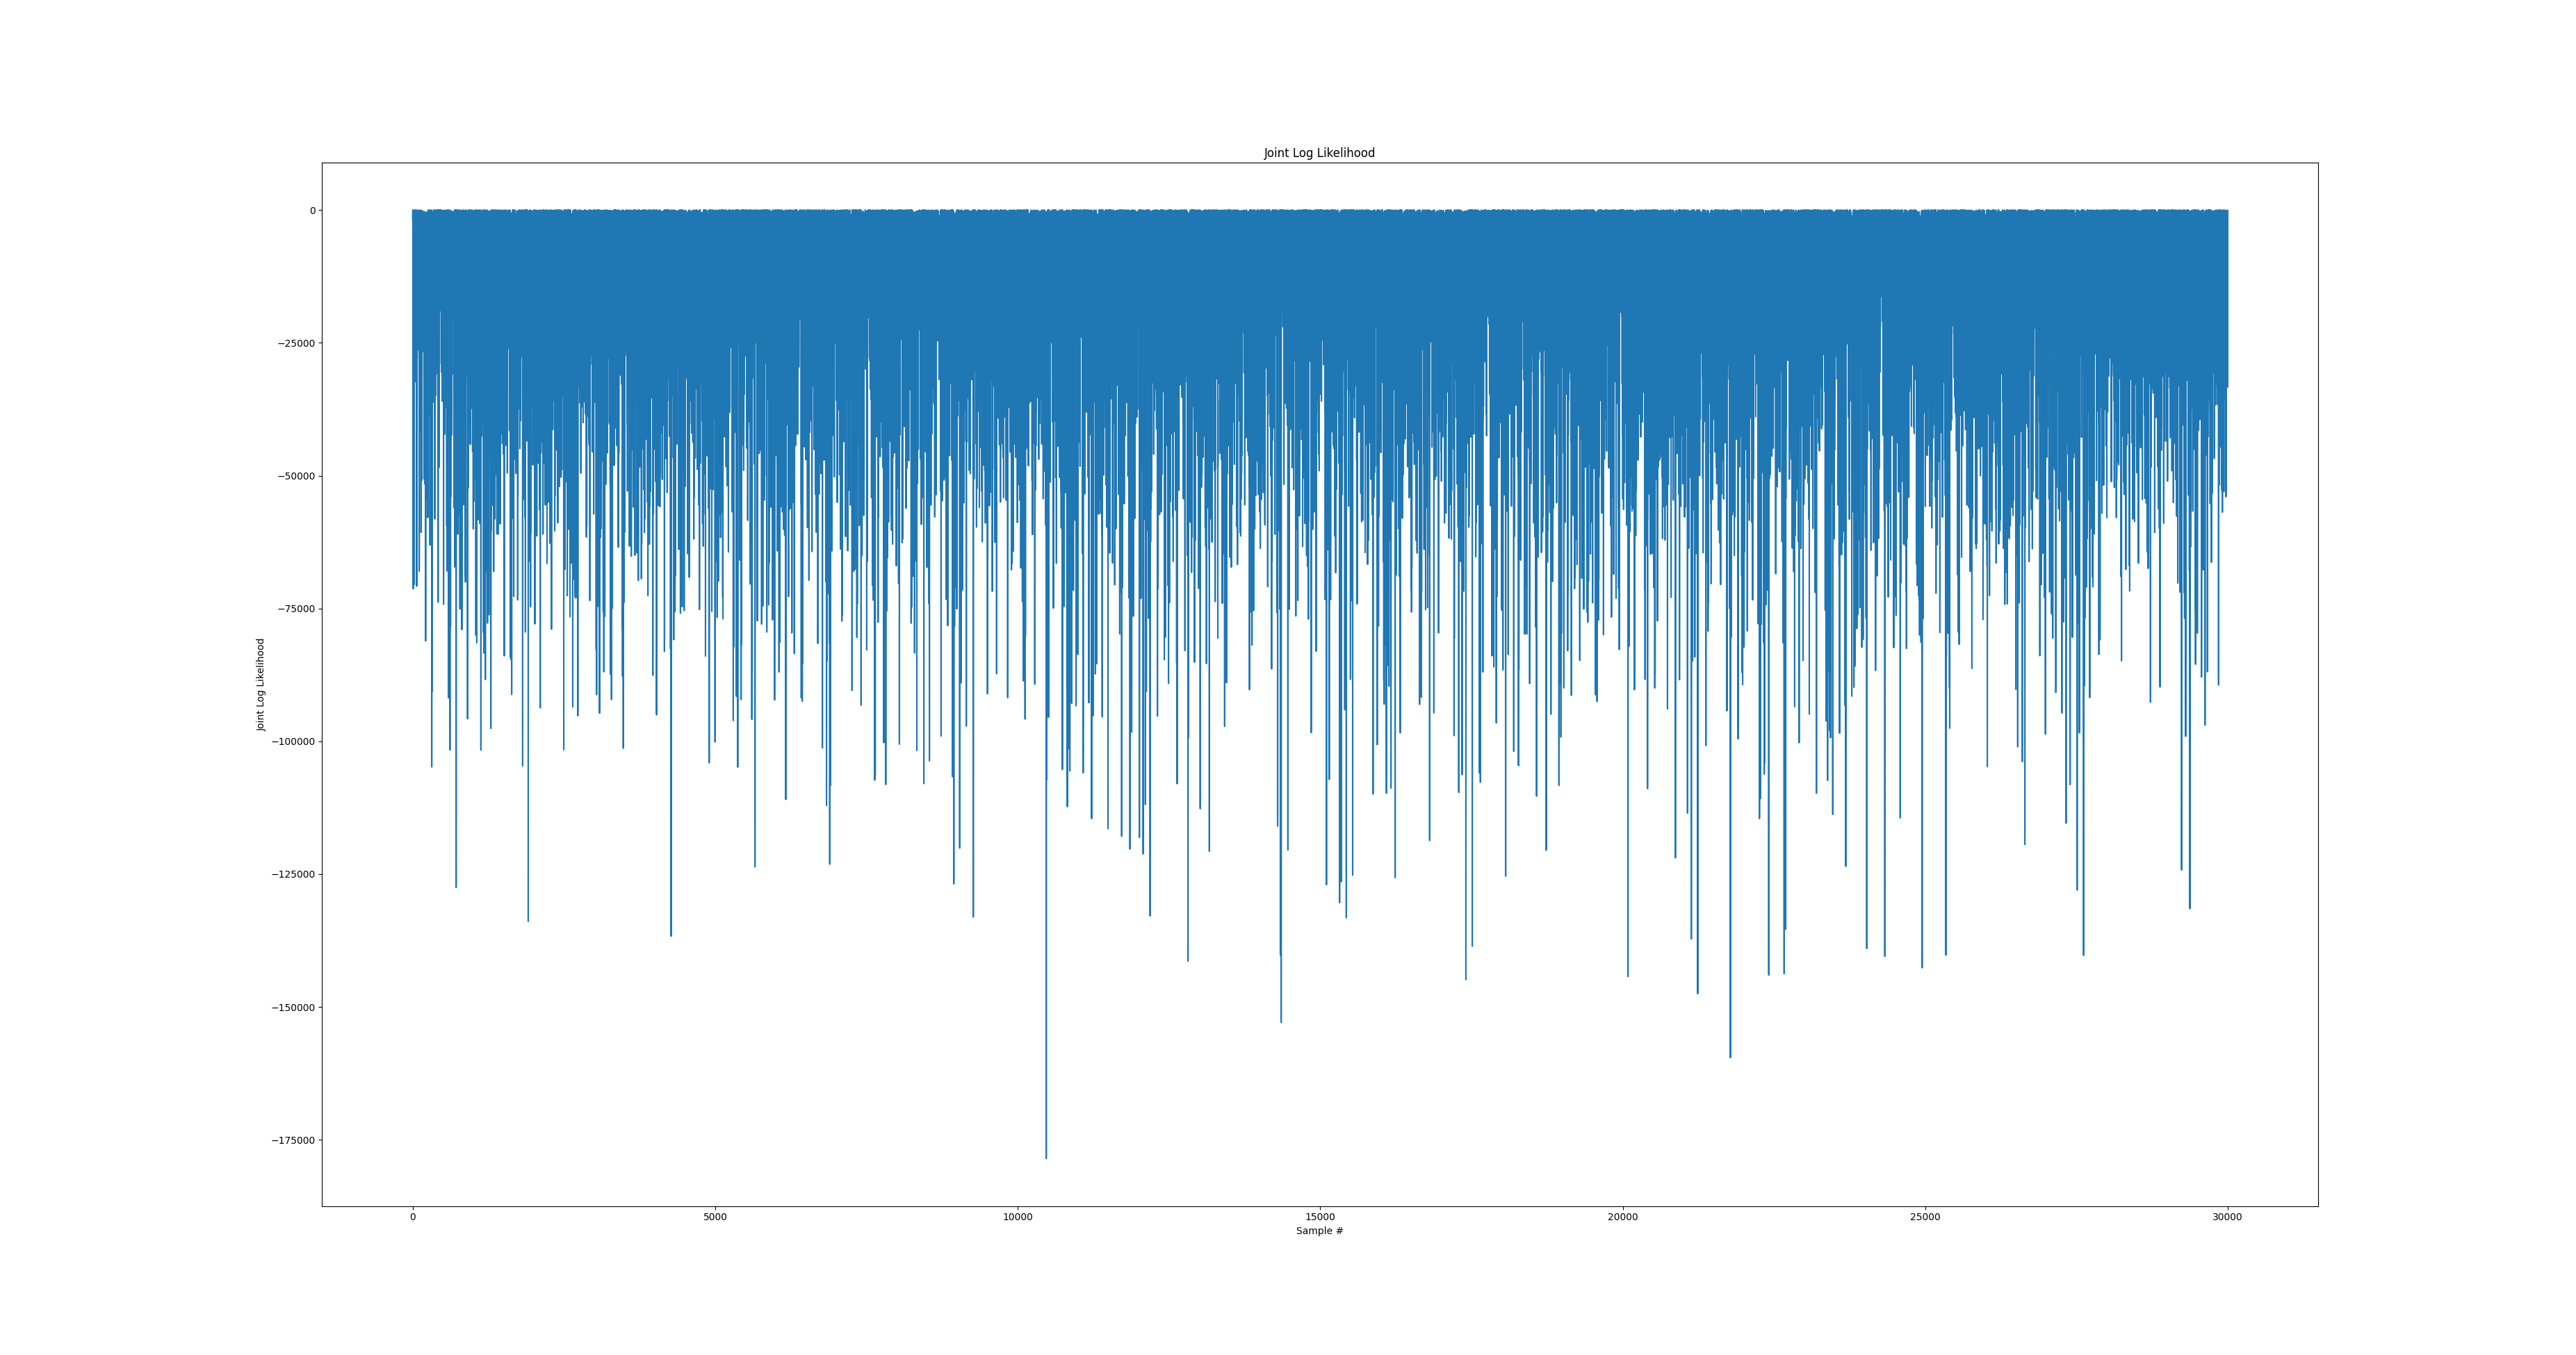
\includegraphics[width=\linewidth]{Figures/p5_ISjll.png}
\end{center}
\section{Metropolis-Hastings within Gibbs (MH-Gibbs)}
This sampler implements algorithm 1 of the textbook using the graph based evaluator. The first thing that happens like in HW2 is a topological sort of the vertices. From the set of vertices, a mapping to the unobserved variables and their link function is created:
\lstinputlisting[language = Python,linerange = {74-79} ]{gibbs.py}
An optimization to speed up computation is to create a mapping of parent nodes from children nodes, i.e. being able to look up in a map what the parents of the current node is:
\lstinputlisting[language = Python,linerange = {164-173} ]{primitives.py}
Then an initial initialization for the unobserved variables $X_0$ is assigned sampling from their prior:
\lstinputlisting[language = Python,linerange = {83-85} ]{gibbs.py}
Then for the specified number of samples, the following loop is run:
\lstinputlisting[language = Python,linerange = {87-99} ]{gibbs.py}
at every Gibbs step, the variables are bound to their expressions in the associated link function, the link function is evaluated to generate a proposal assignment, the acceptance ratio for a one step MH is computed and the proposed sample is either accepted or rejected.
 \lstinputlisting[language = Python,linerange = {39-49} ]{gibbs.py}
In order to compute the acceptance ratio, we first need to compute the Markov blanket of the variable in question from the graph:
\lstinputlisting[language = Python,linerange = {103-126} ]{gibbs.py}
The variables returned from the Markov blanket are scored and the acceptance ratio is returned:
\lstinputlisting[language = Python,linerange = {14-37} ]{gibbs.py}
Each program is run with 30k samples, except for program 3 which runs much much slower and thus only has 8k samples.
\subsection{Program 1}
\begin{verbatim}
Collect samples denoted by program 1:
Elapsed time for program  1 .daphne is:  0:00:35.695762  seconds
tensor([3.5825, 3.5825, 3.5825,  ..., 6.6816, 6.6816, 6.6816])
Mean of trace:  tensor(7.2390)  
and variance of trace:  tensor(0.7177)
\end{verbatim}
\begin{center}
	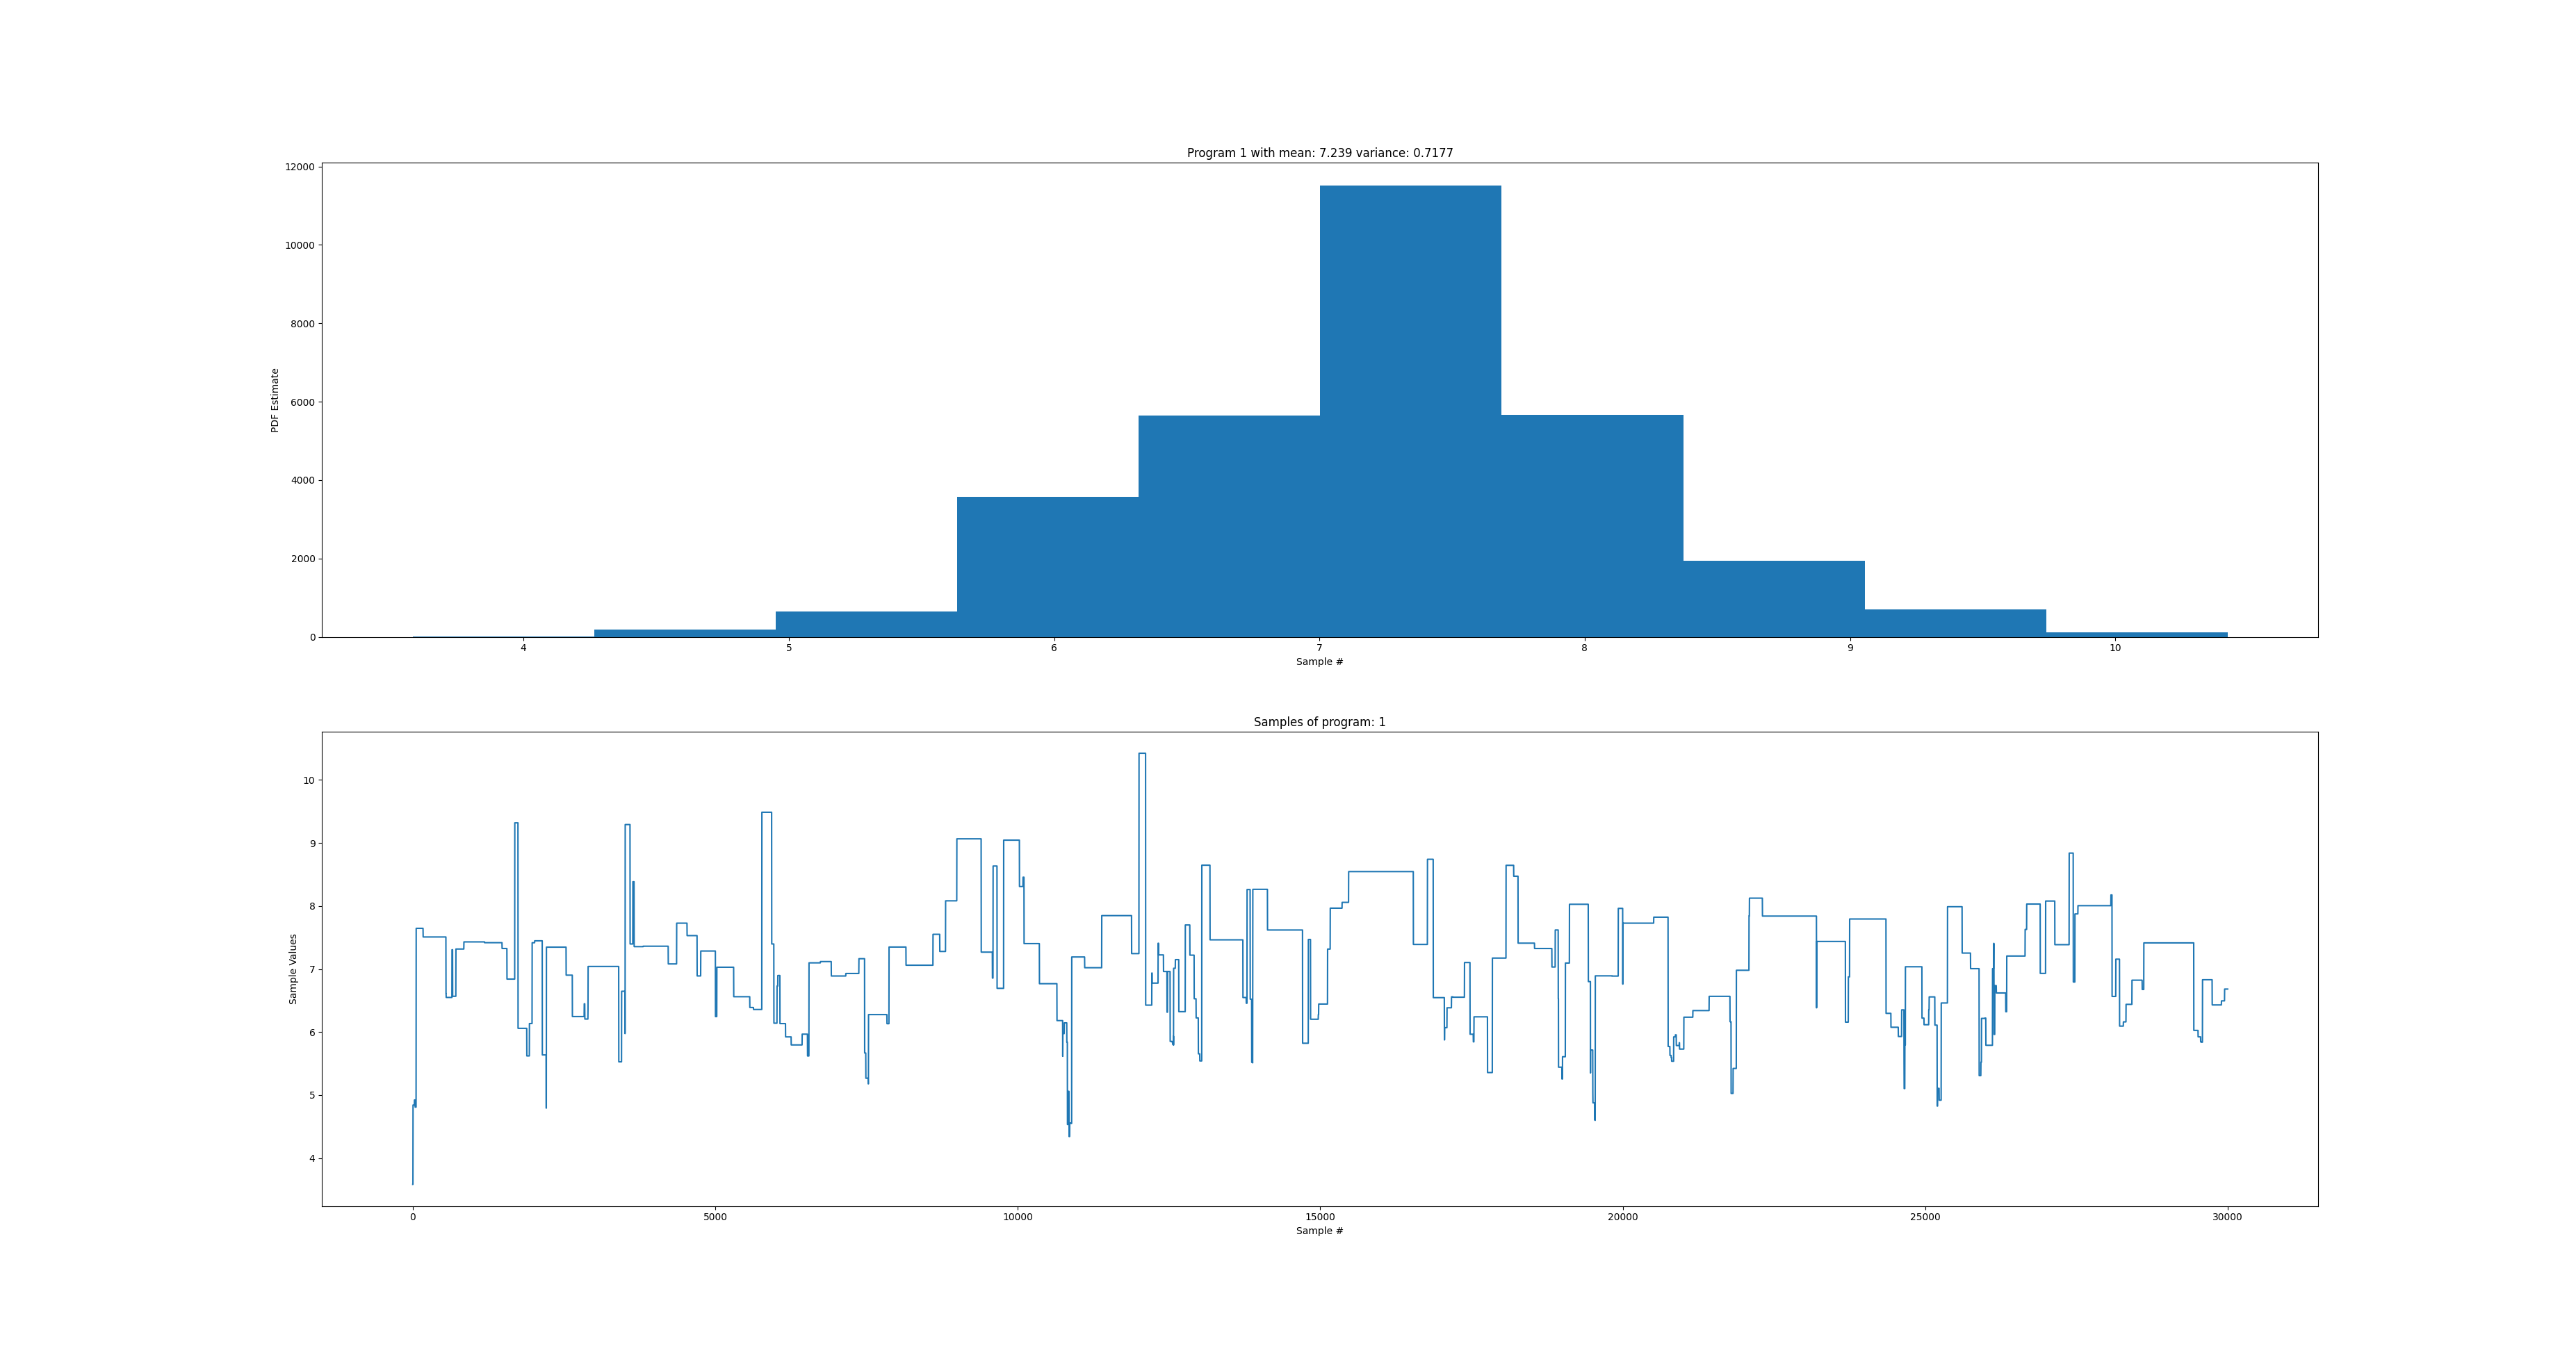
\includegraphics[width=\linewidth]{Figures/p1_MHGibbs.png}
\end{center}
\begin{center}
	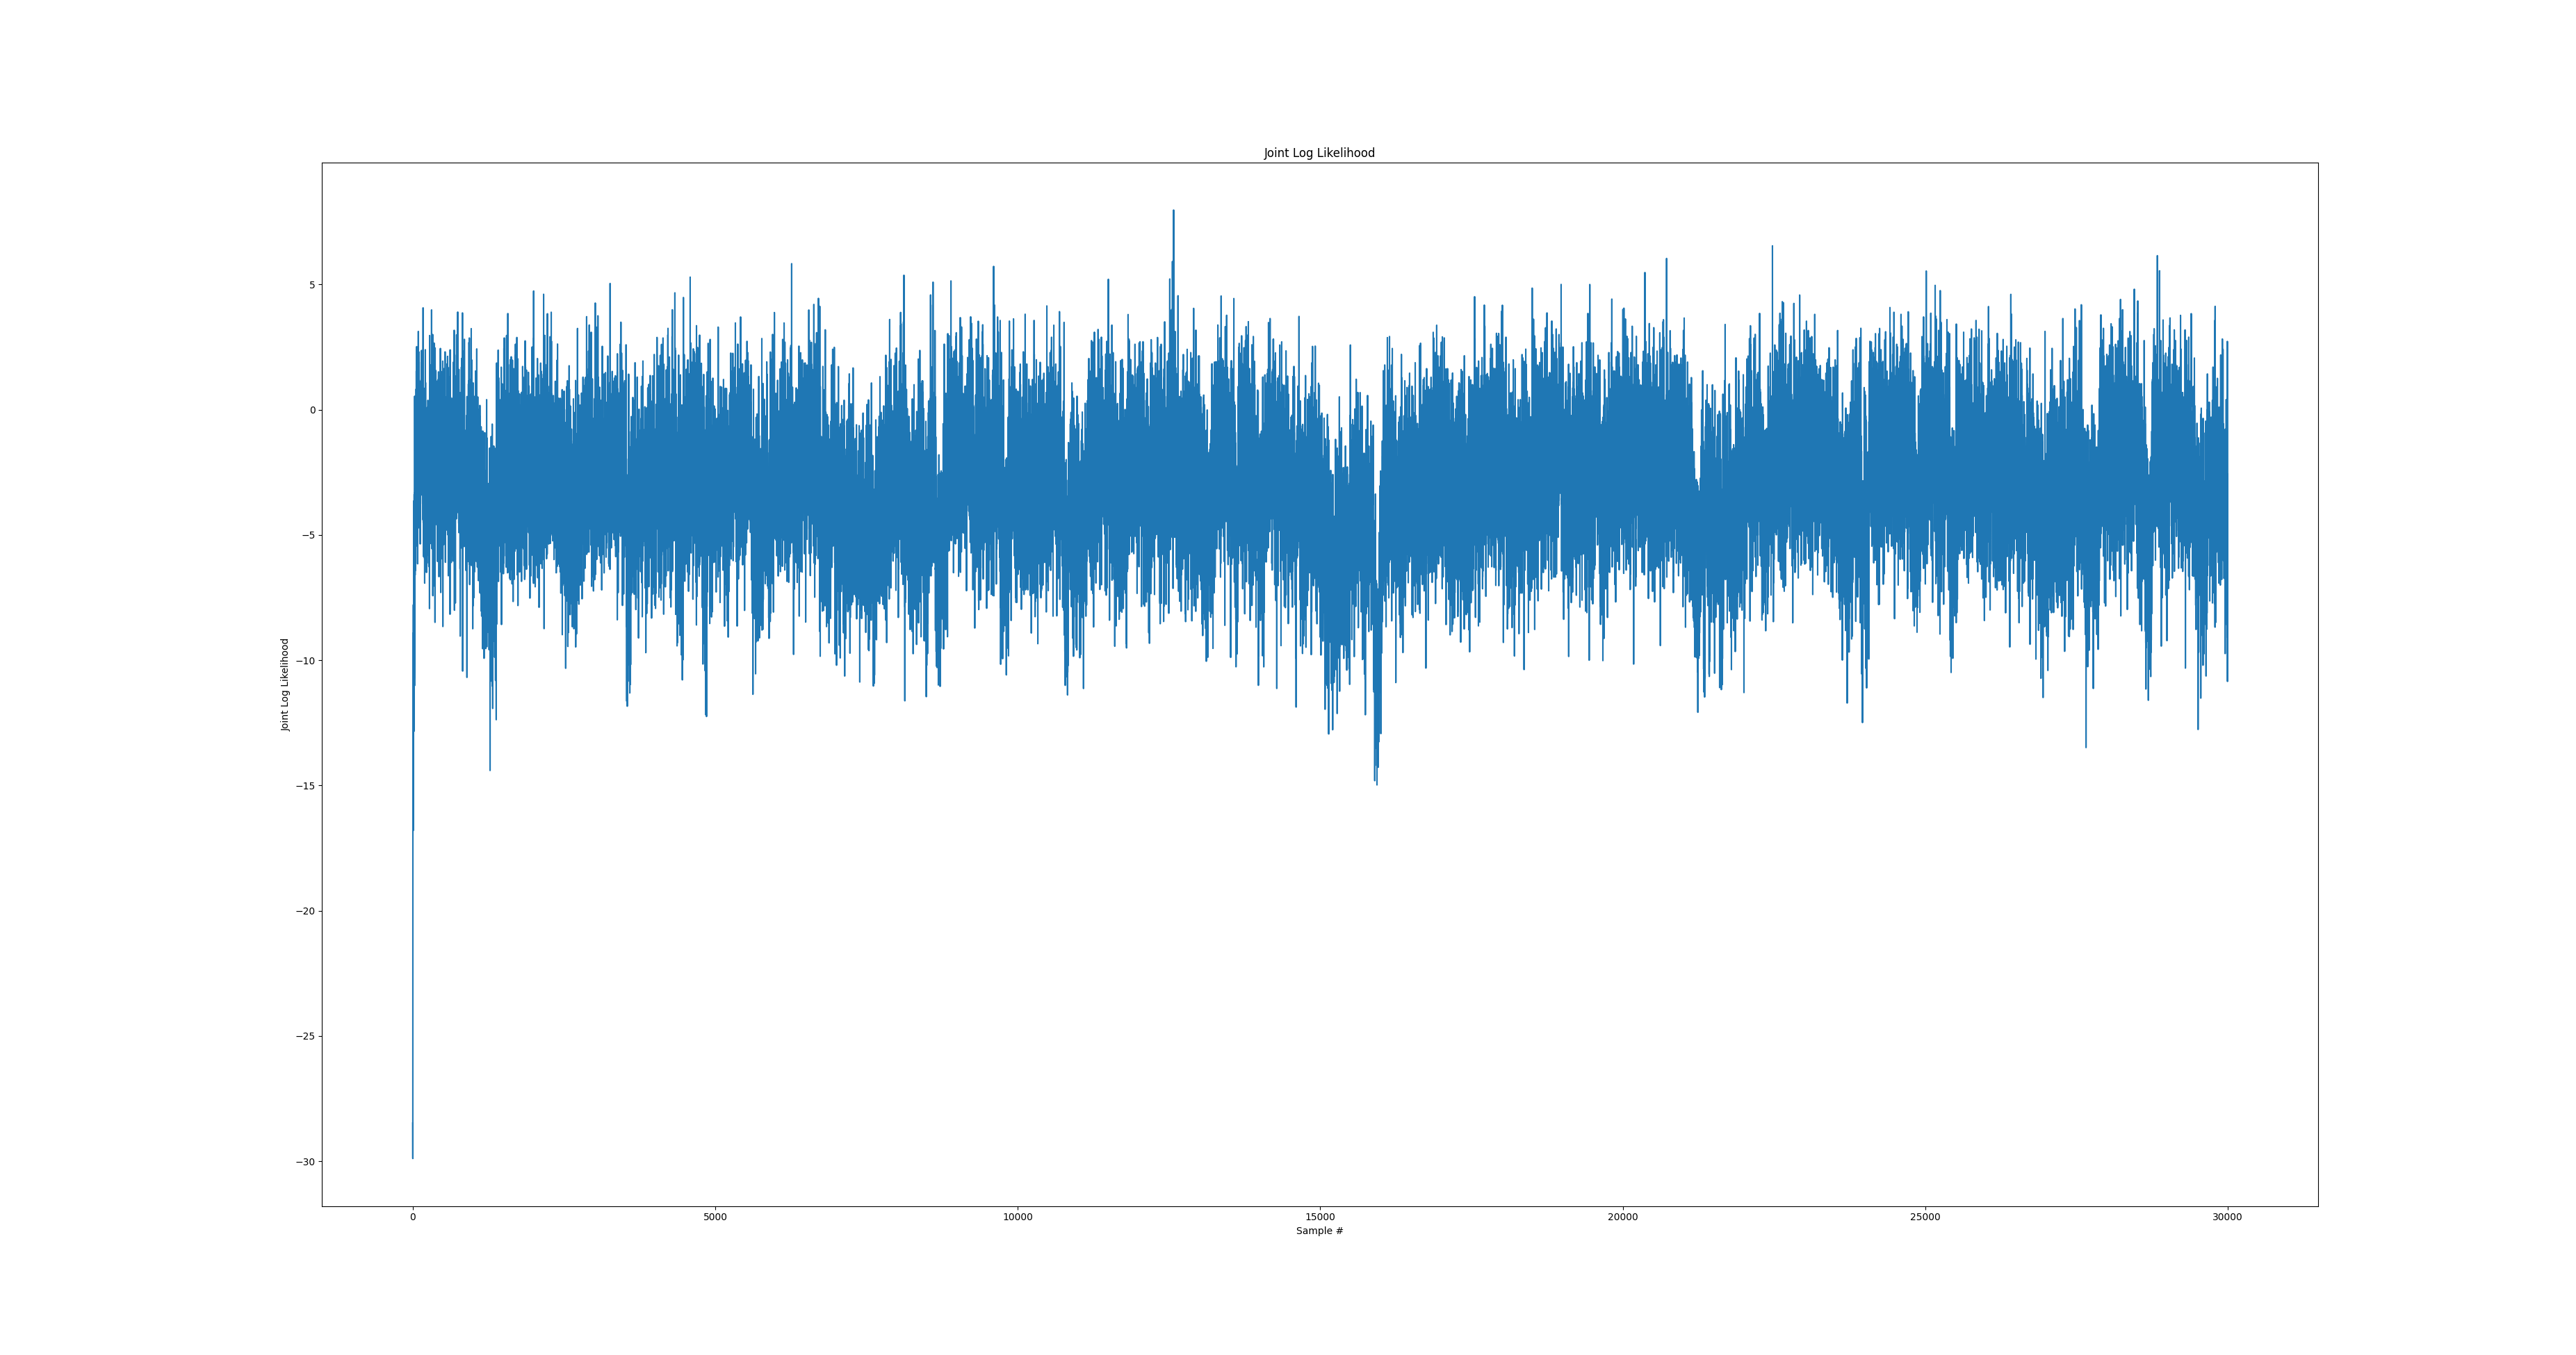
\includegraphics[width=\linewidth]{Figures/p1_MHGibbsjll.png}
\end{center}
\subsection{Program 2}
\begin{verbatim}
Collect samples denoted by program 2:
Elapsed time for program  2 .daphne is:  0:02:54.739333  seconds
tensor([[ 4.1943, -4.8585],
[ 4.1943, -4.8585],
[ 4.1943, -4.8585],
...,
[ 2.1528, -0.3358],
[ 2.1528, -0.3358],
[ 2.1528, -0.3358]])
Mean of trace:  tensor([ 2.0691, -0.2042])  
and variance of trace:  tensor([0.0838, 1.2141])
The covariance matrix:  
[[ 0.08381463 -0.29515154]
[-0.29515154  1.21406202]]
\end{verbatim}
\begin{center}
	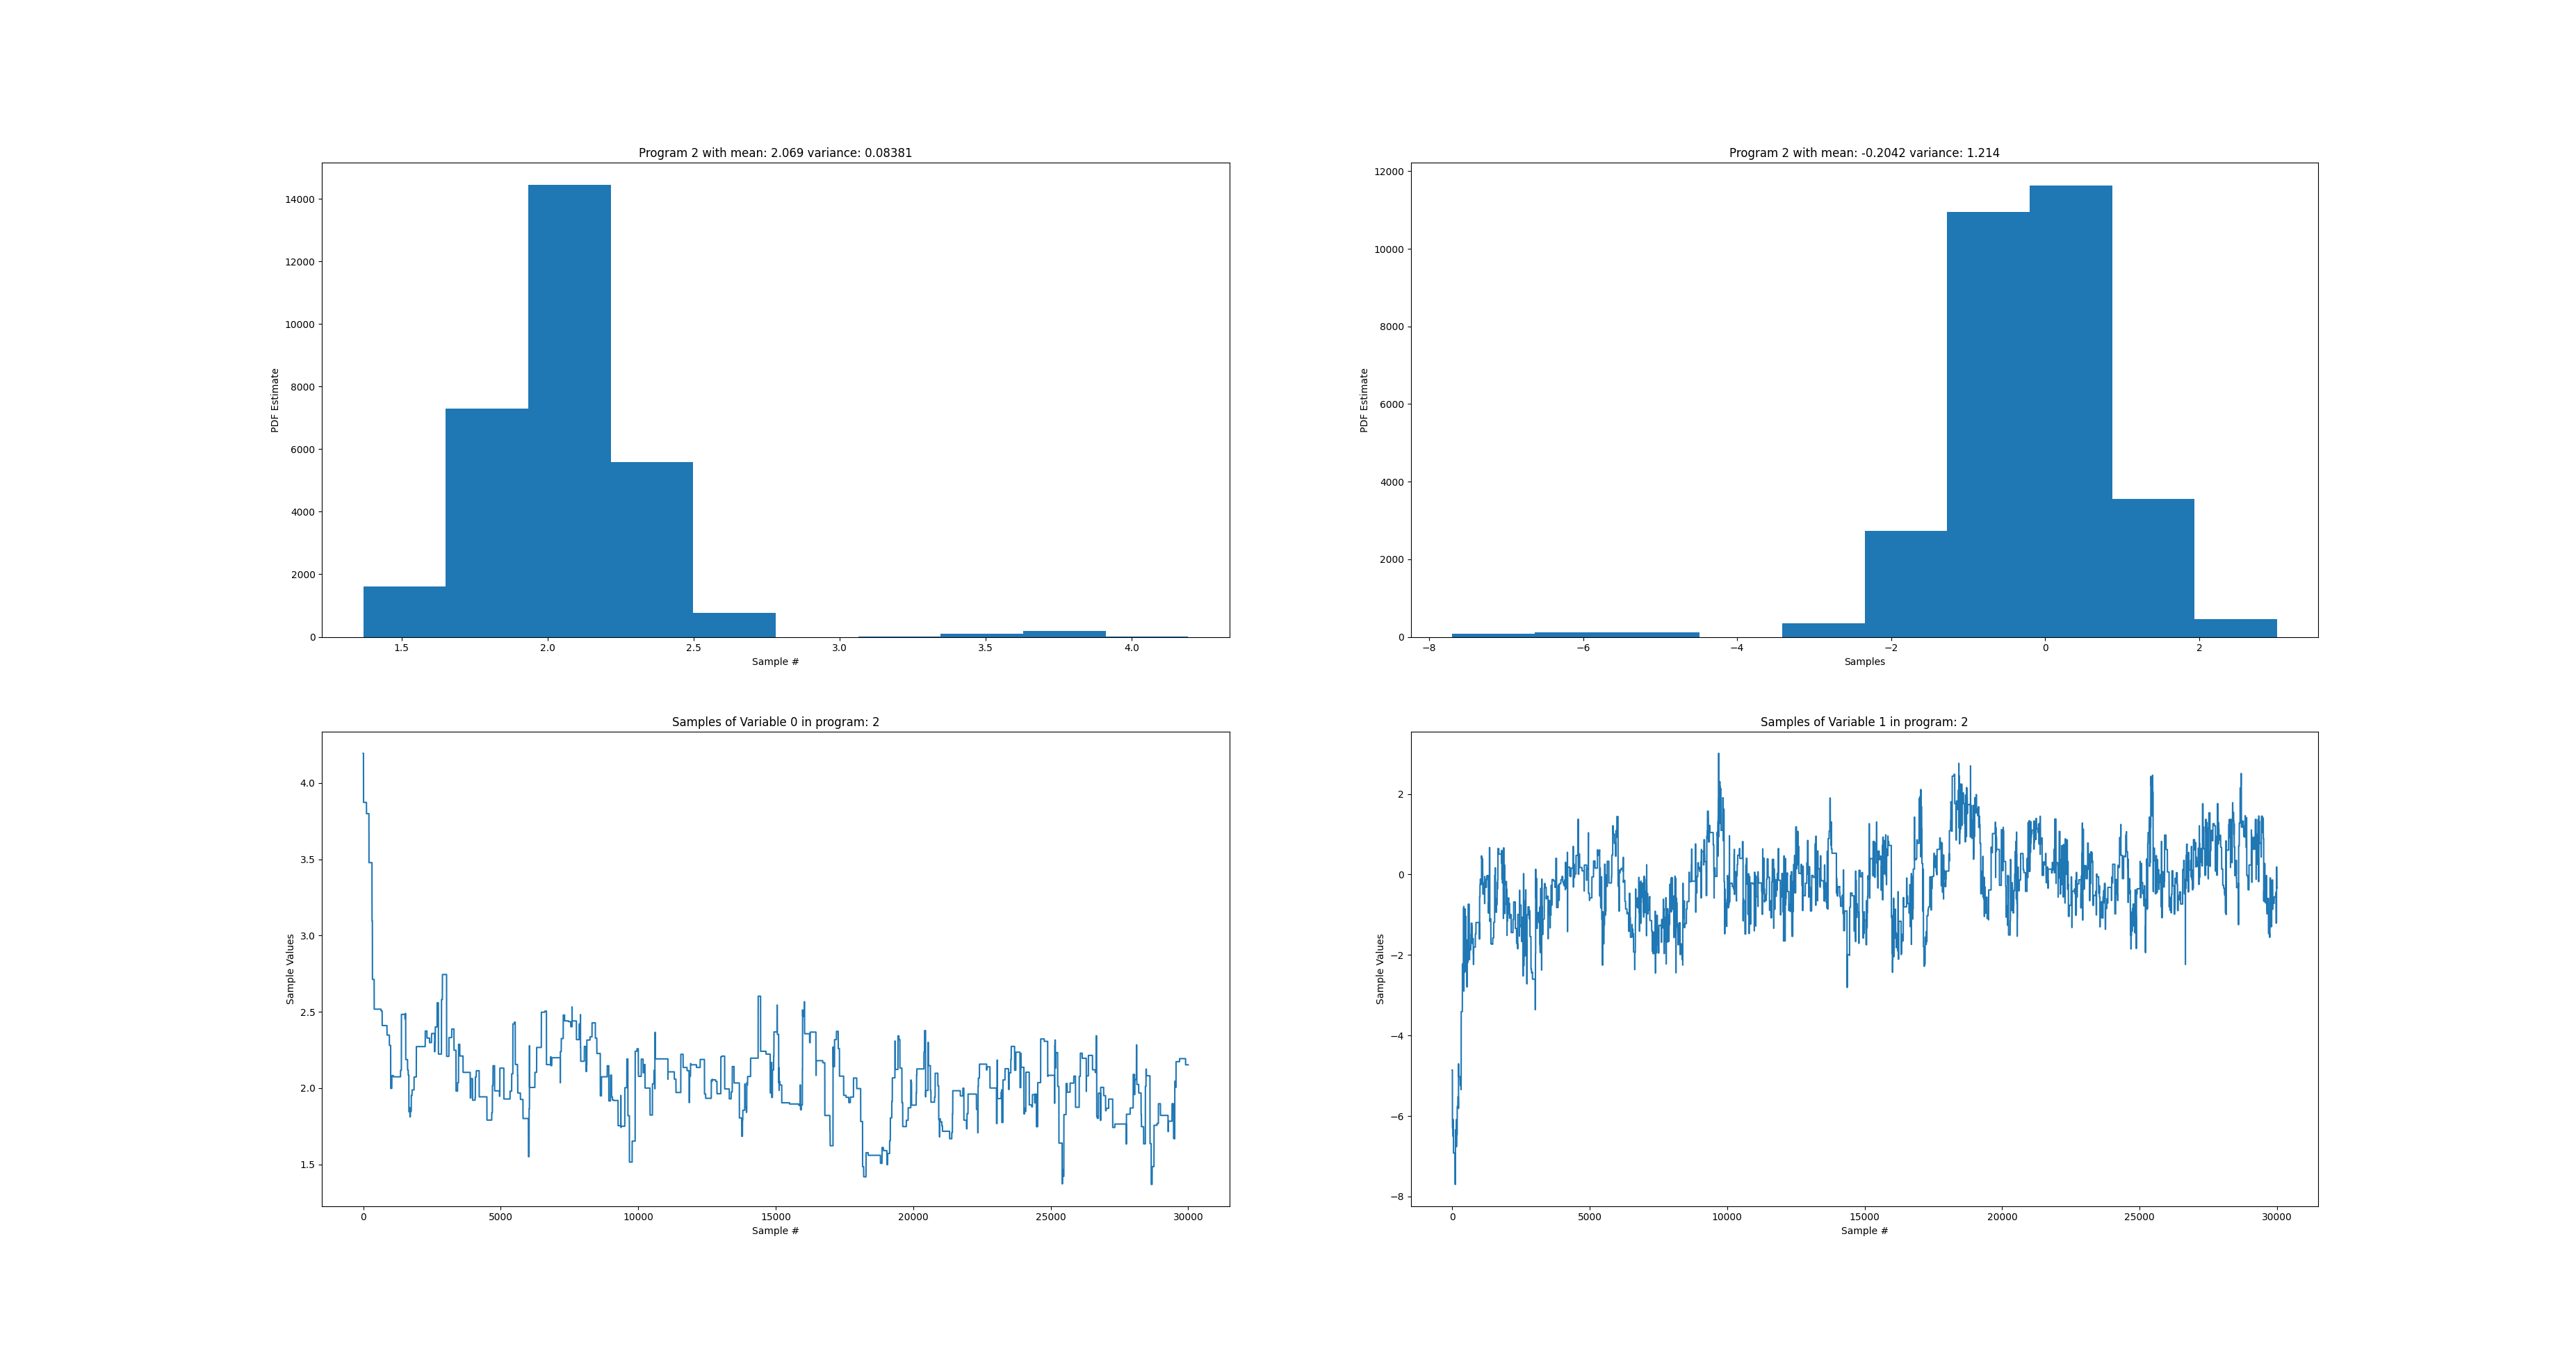
\includegraphics[width=\linewidth]{Figures/p2_MHGibbs.png}
\end{center}
\begin{center}
	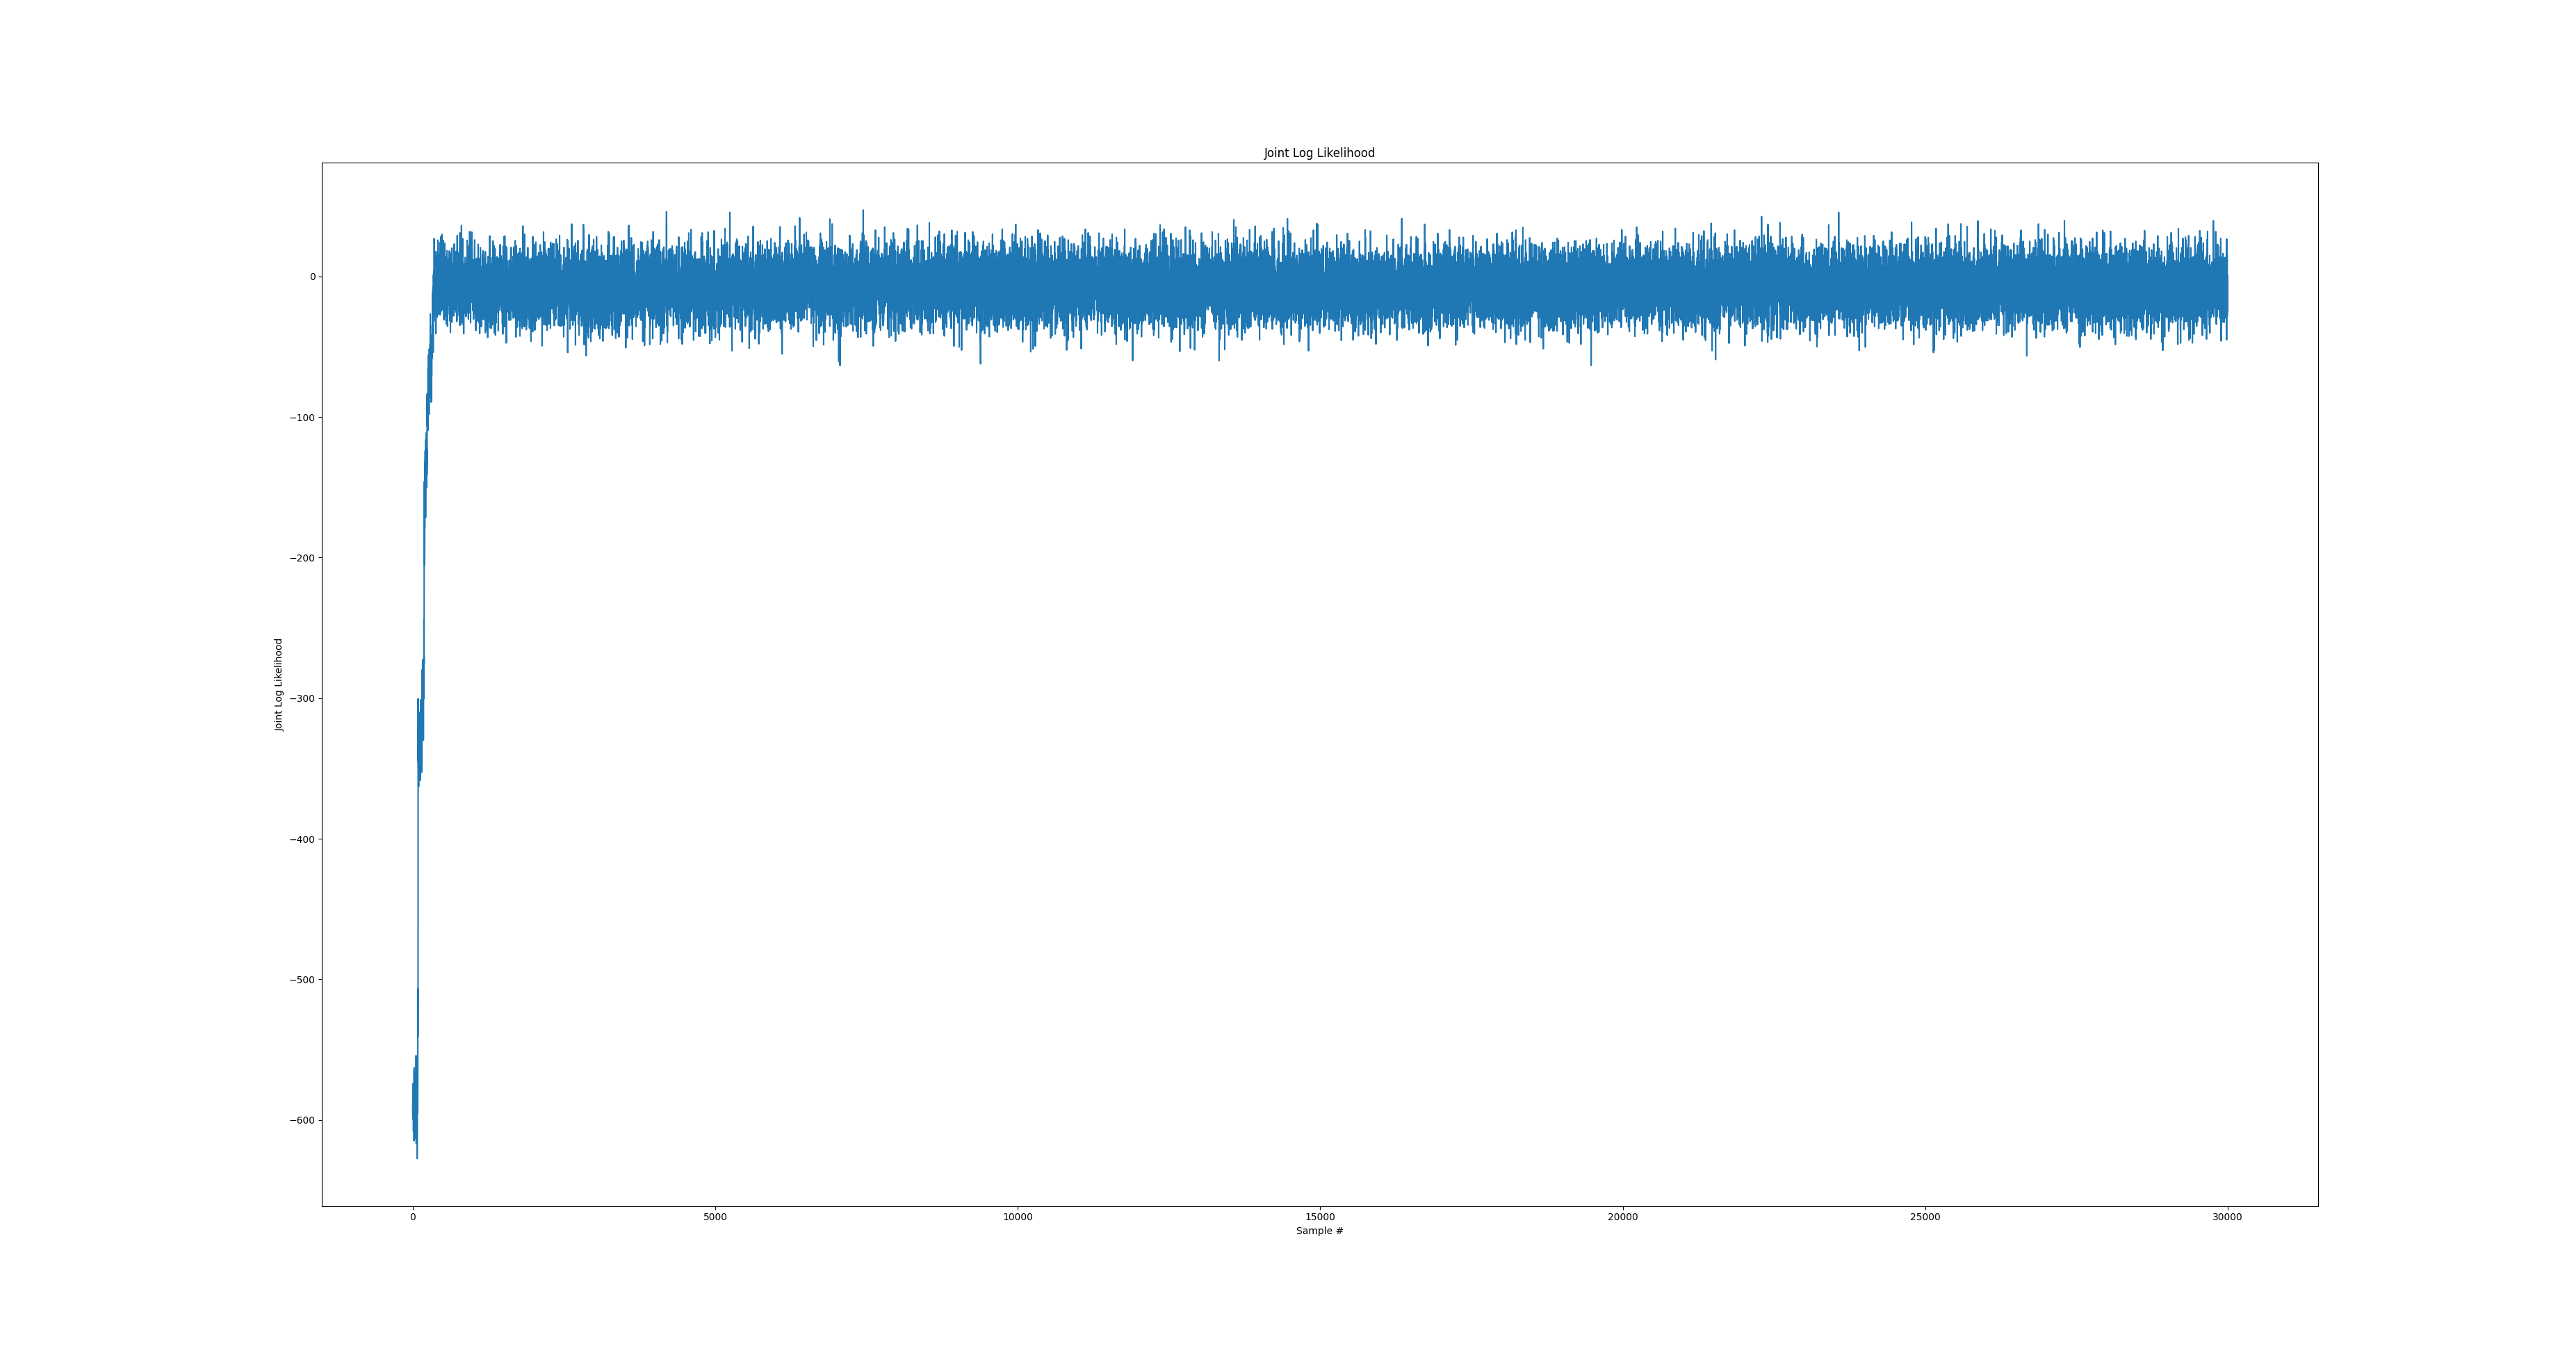
\includegraphics[width=\linewidth]{Figures/p2_MHGibbsjll.png}
\end{center}
\subsection{Program 3}
\begin{verbatim}
Collect samples denoted by program 3:
Elapsed time for program  3 .daphne is:  0:11:39.550165  seconds
tensor([1., 0., 1.,  ..., 1., 1., 1.])
Mean of trace:  tensor(0.6874)  
and variance of trace:  tensor(0.2149)
\end{verbatim}
\begin{center}
	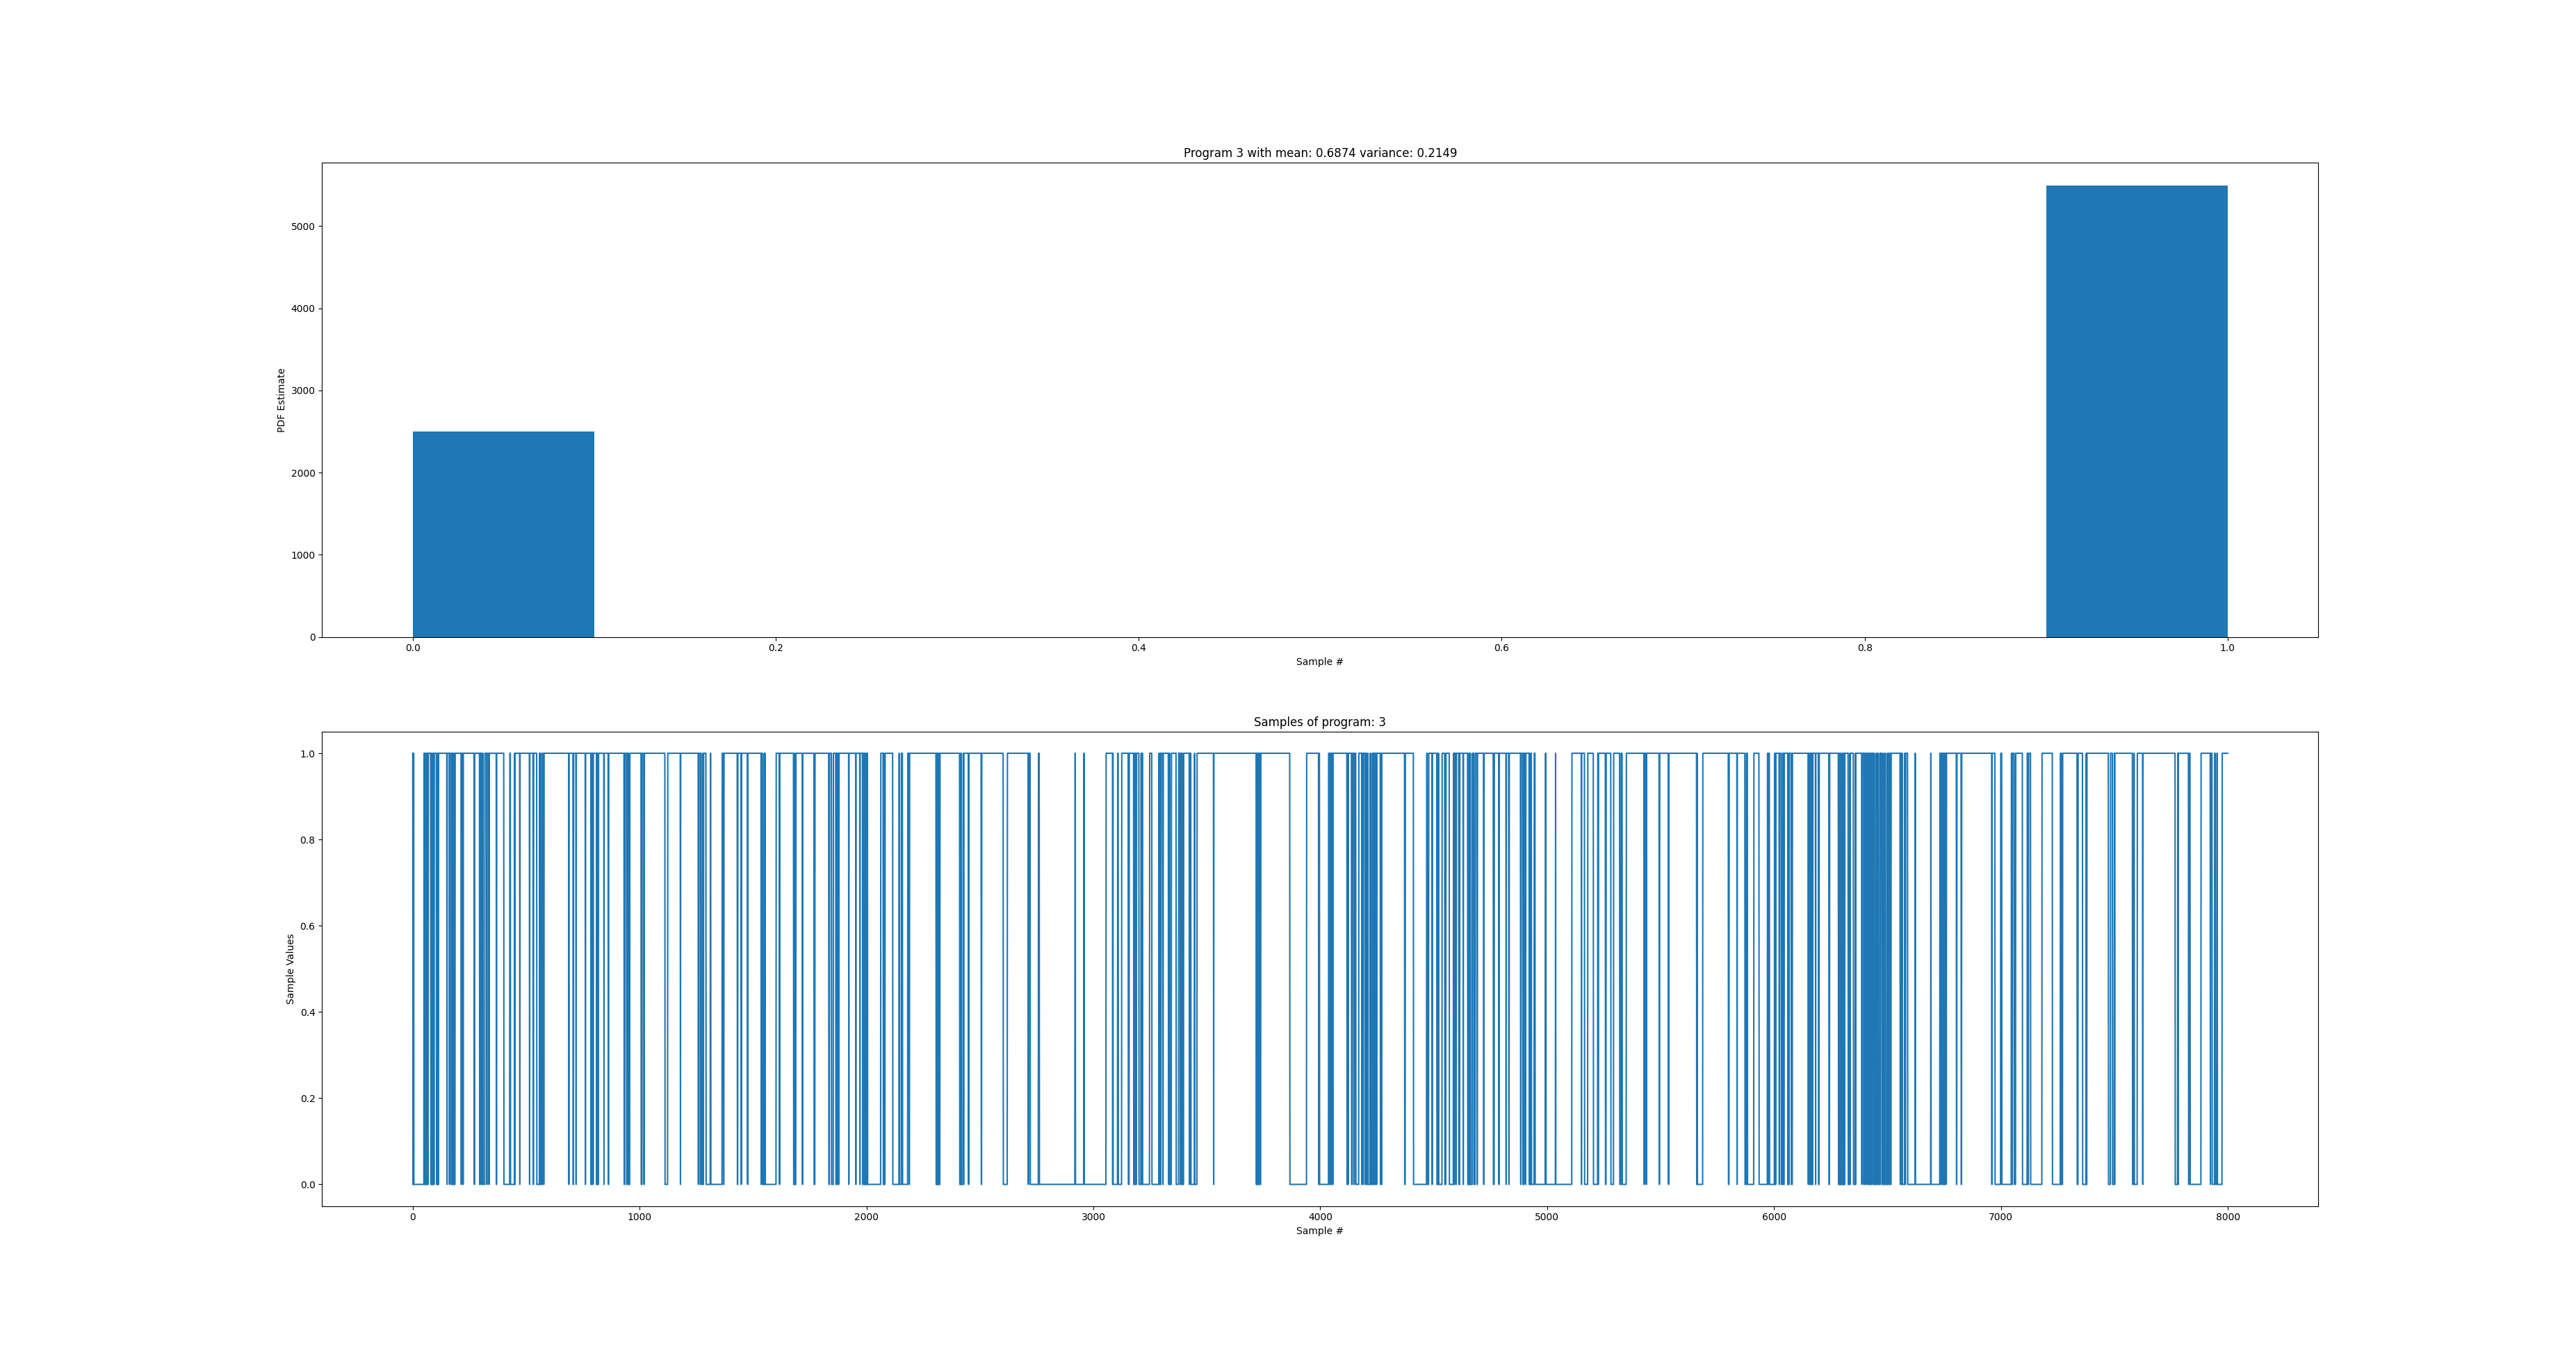
\includegraphics[width=\linewidth]{Figures/p3_MHGibbs.png}
\end{center}
\begin{center}
	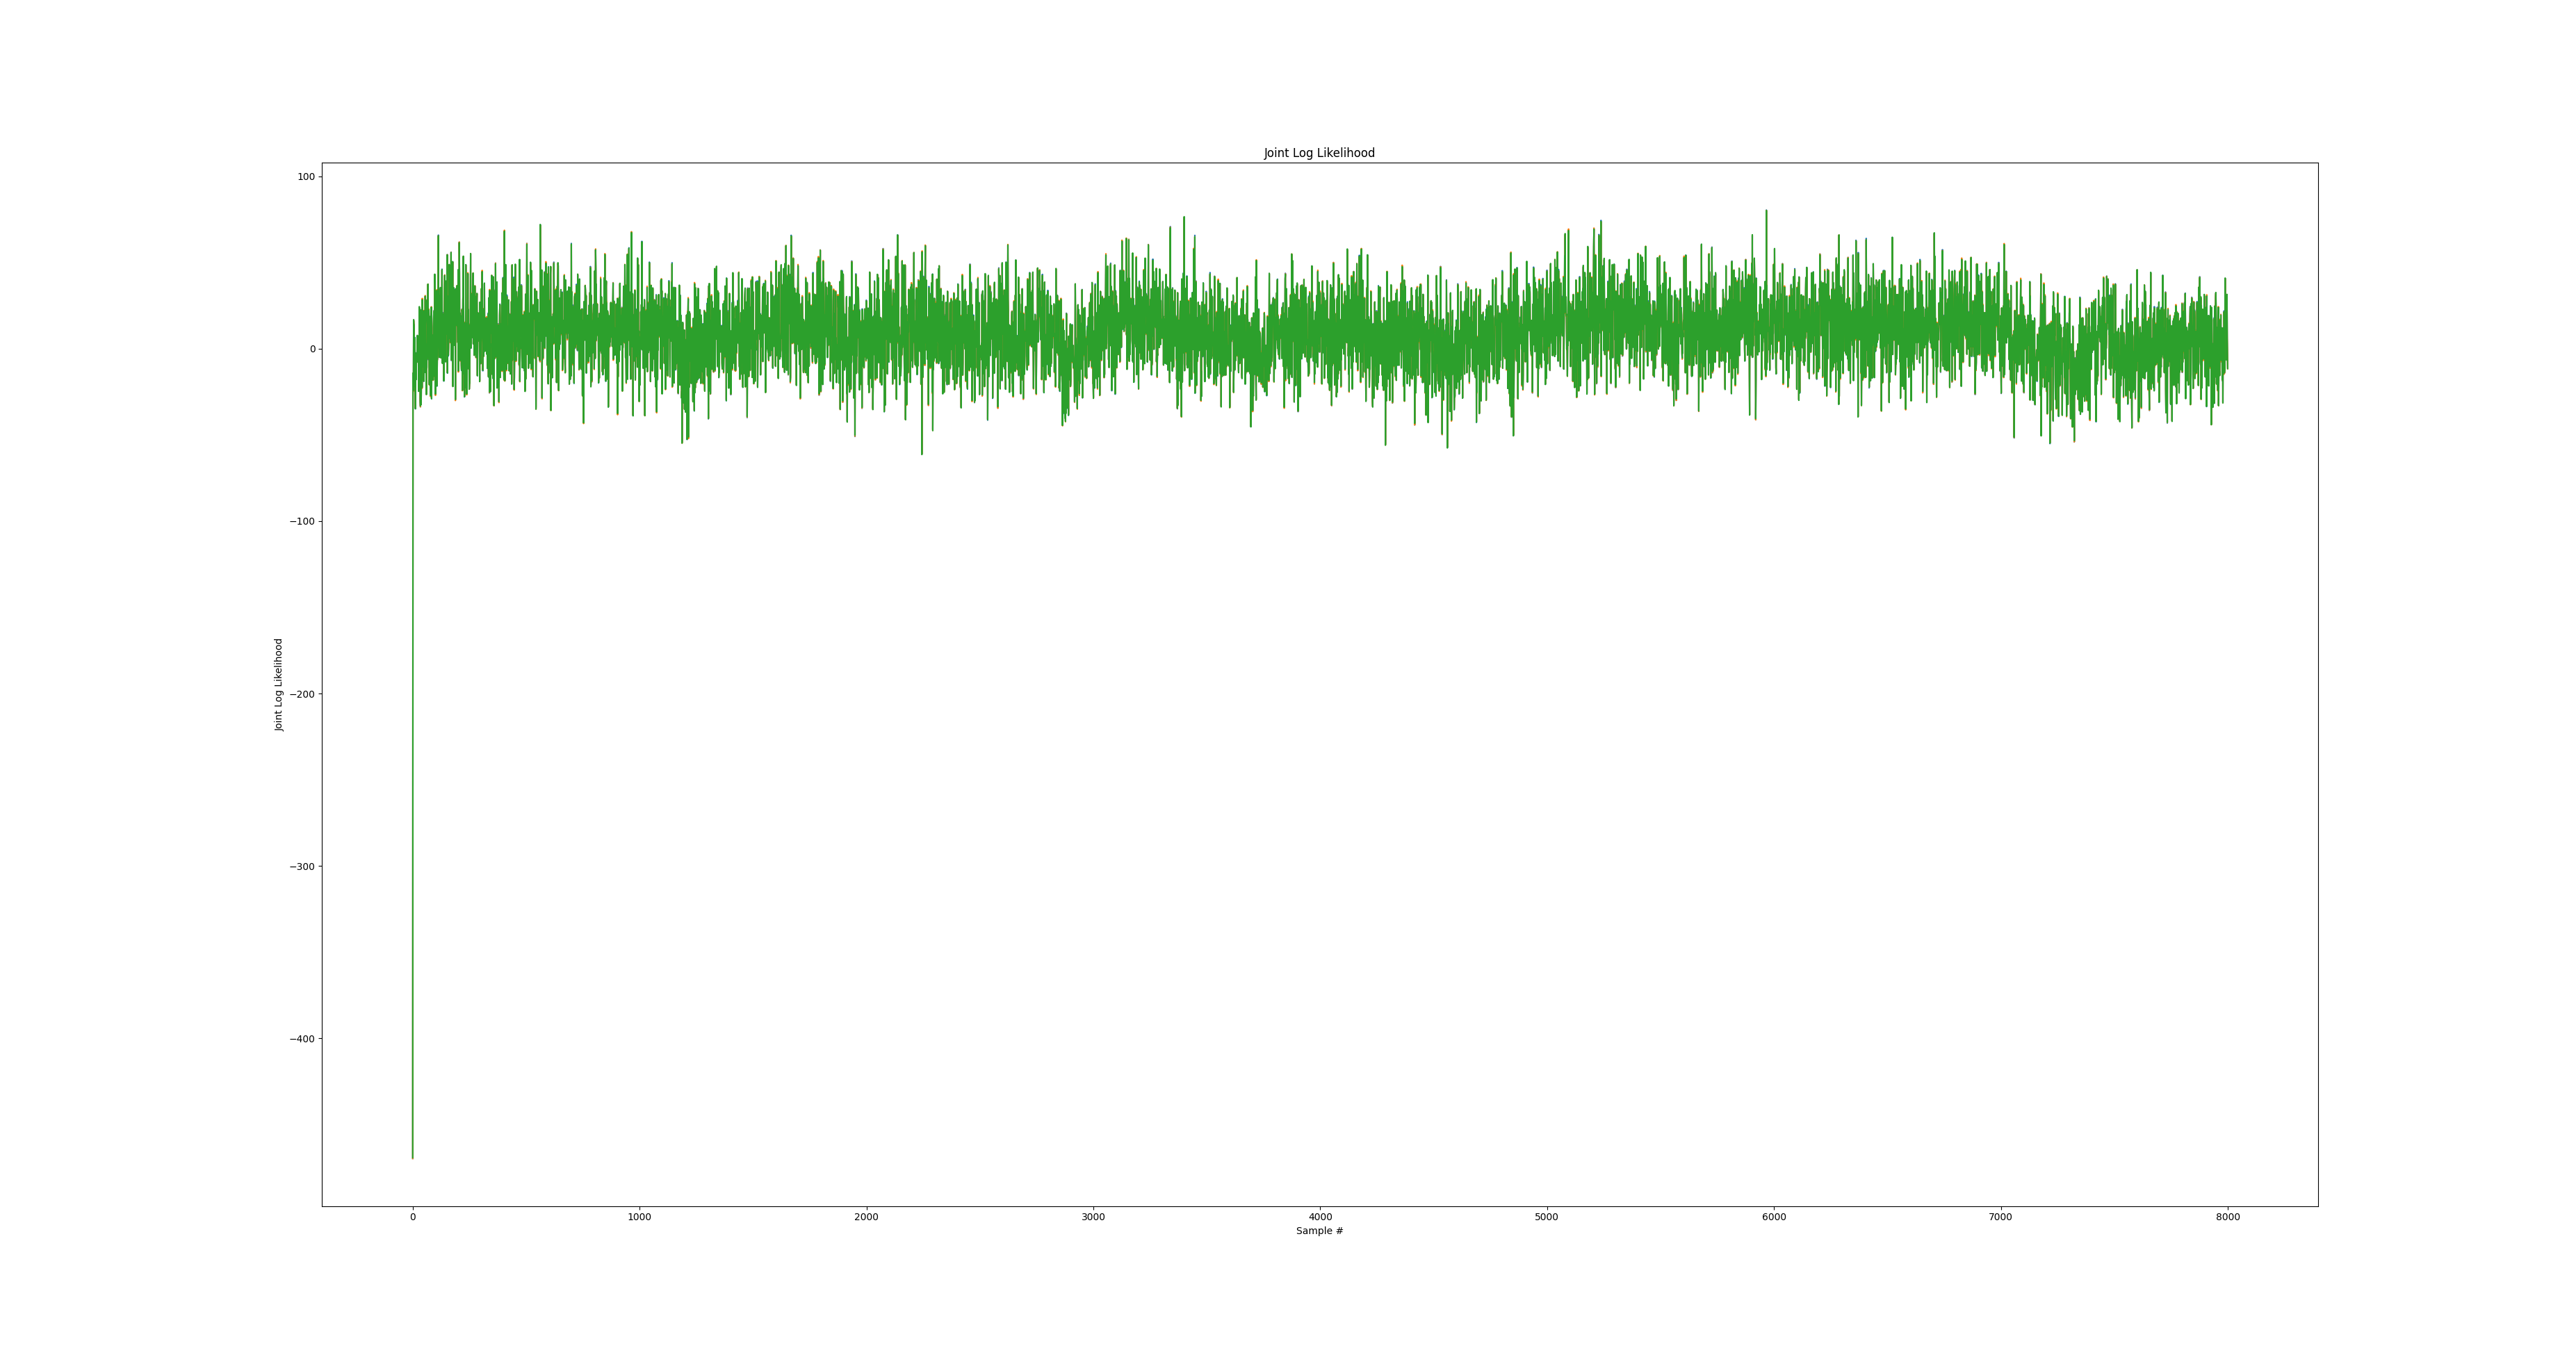
\includegraphics[width=\linewidth]{Figures/p3_MHGibbsjll.png}
\end{center}
\subsection{Program 4}
\begin{verbatim}
Collect samples denoted by program 4:
Elapsed time for program  4 .daphne is:  0:04:13.502343  seconds
tensor([0., 0., 0.,  ..., 1., 1., 0.])
Mean of trace:  tensor(0.3175)  
and variance of trace:  tensor(0.2167)
\end{verbatim}
\begin{center}
	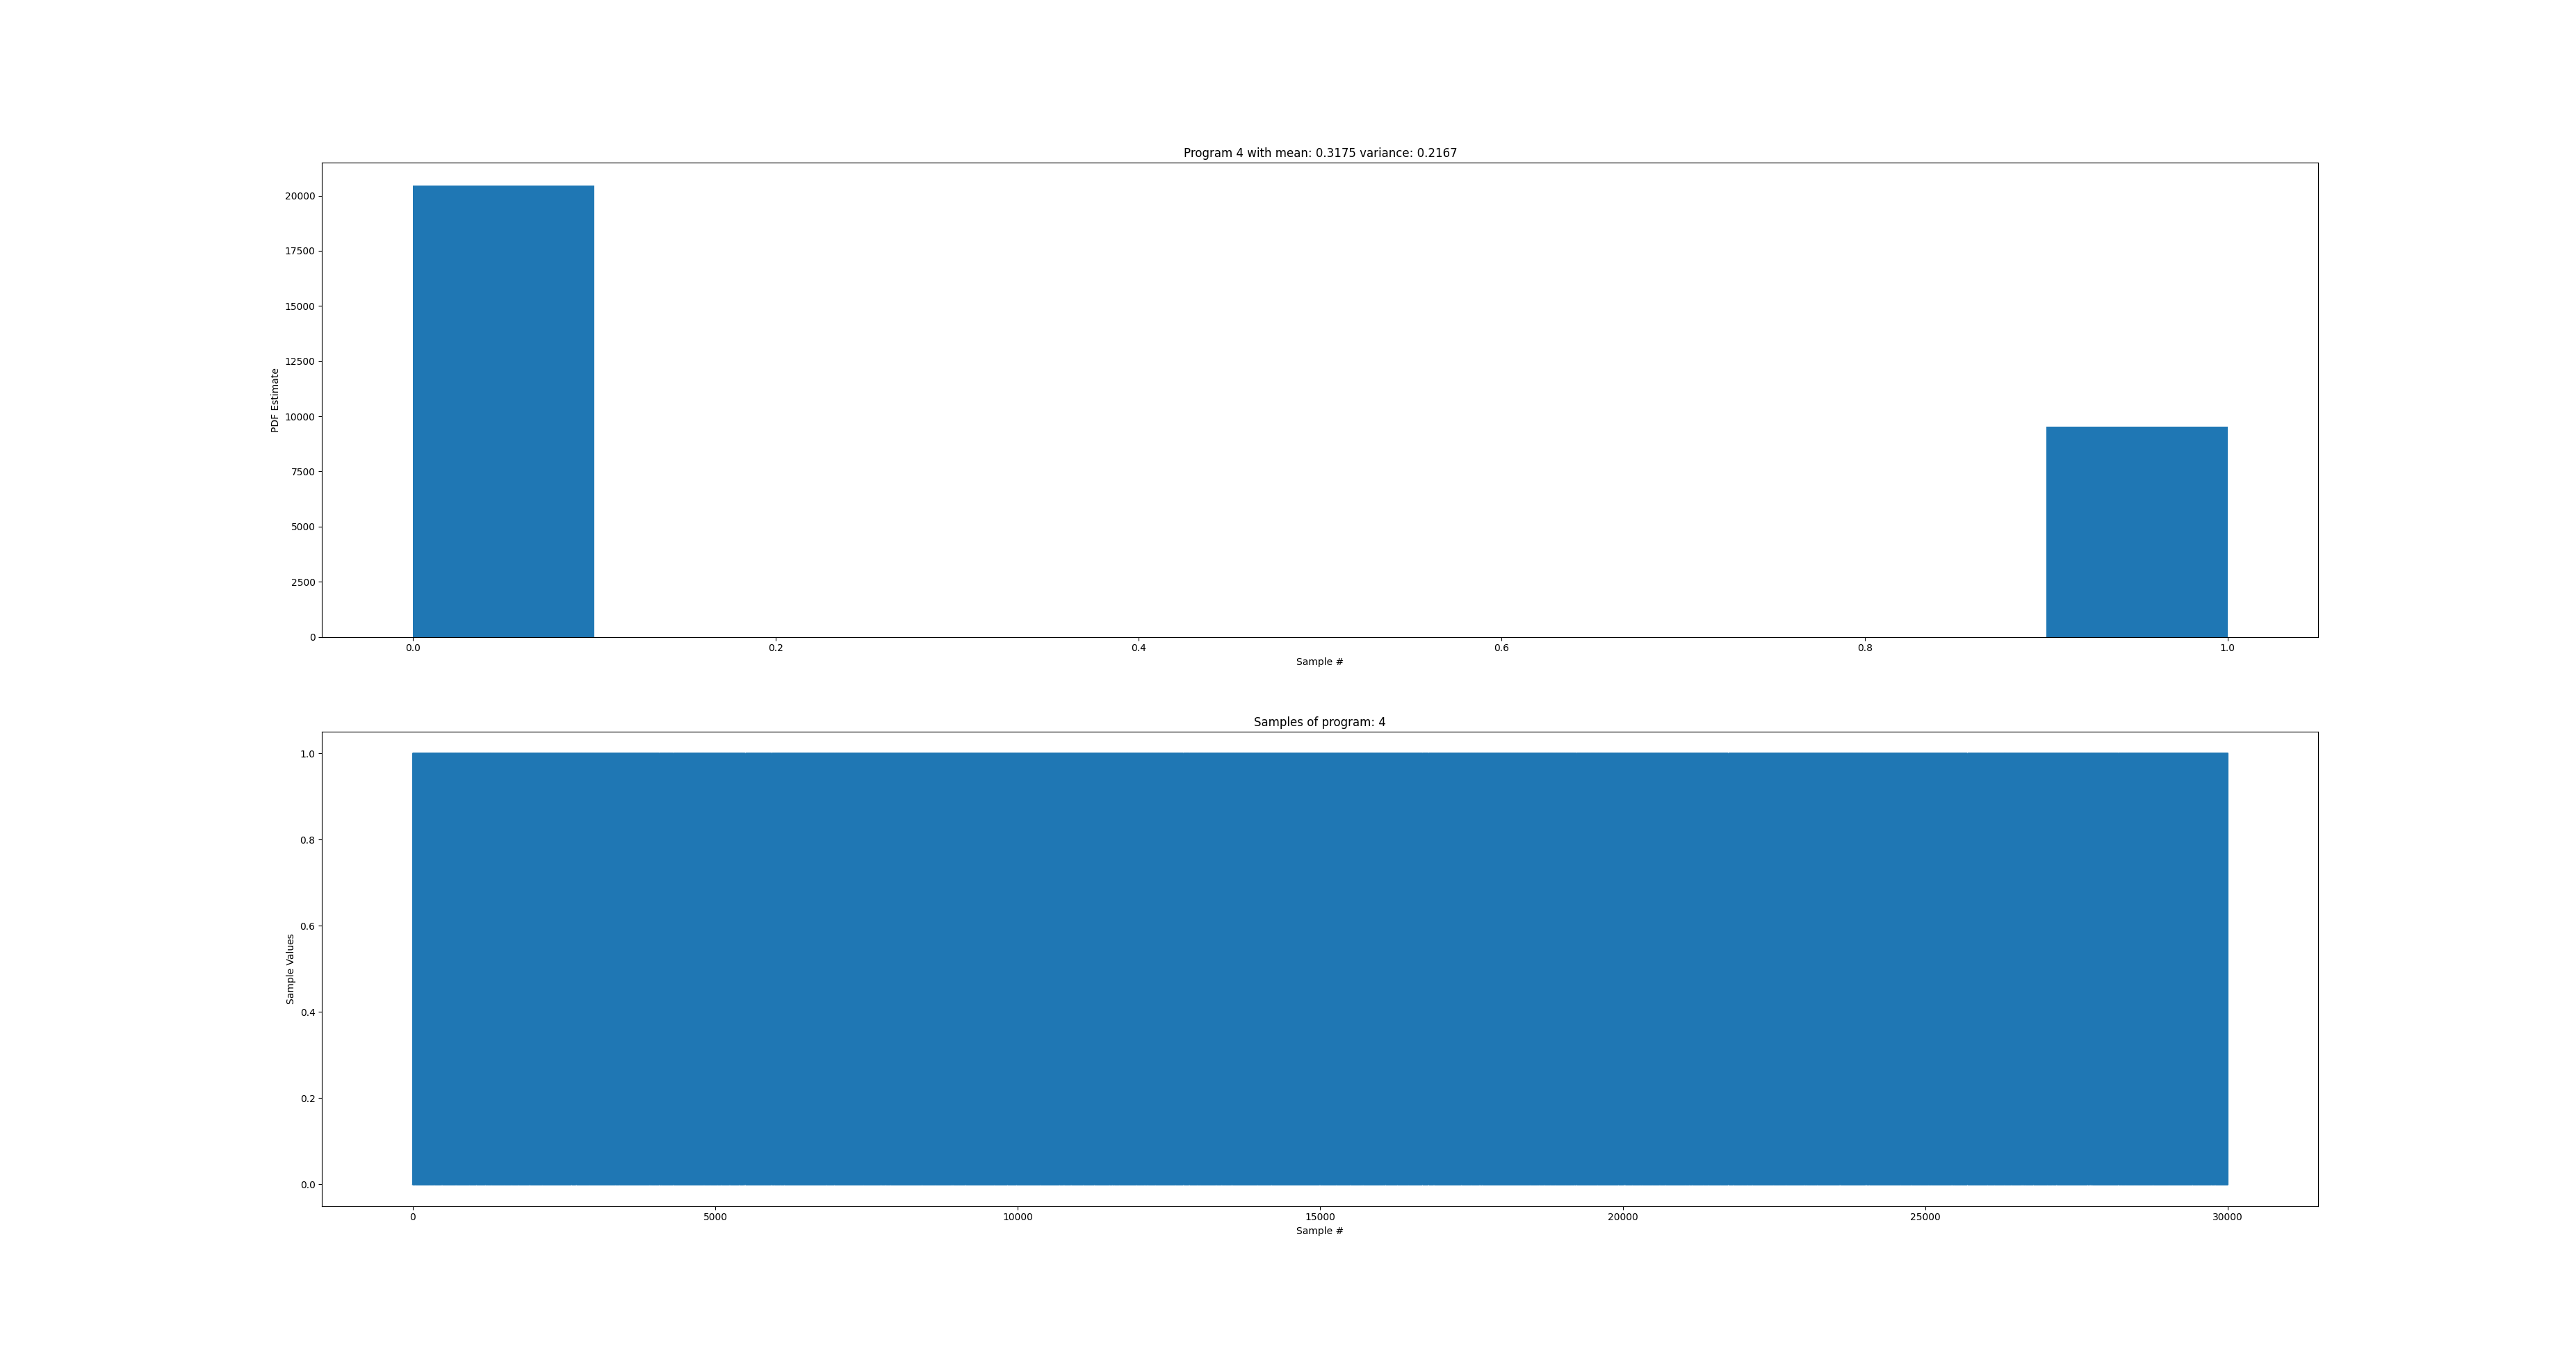
\includegraphics[width=\linewidth]{Figures/p4_MHGibbs.png}
\end{center}
\begin{center}
	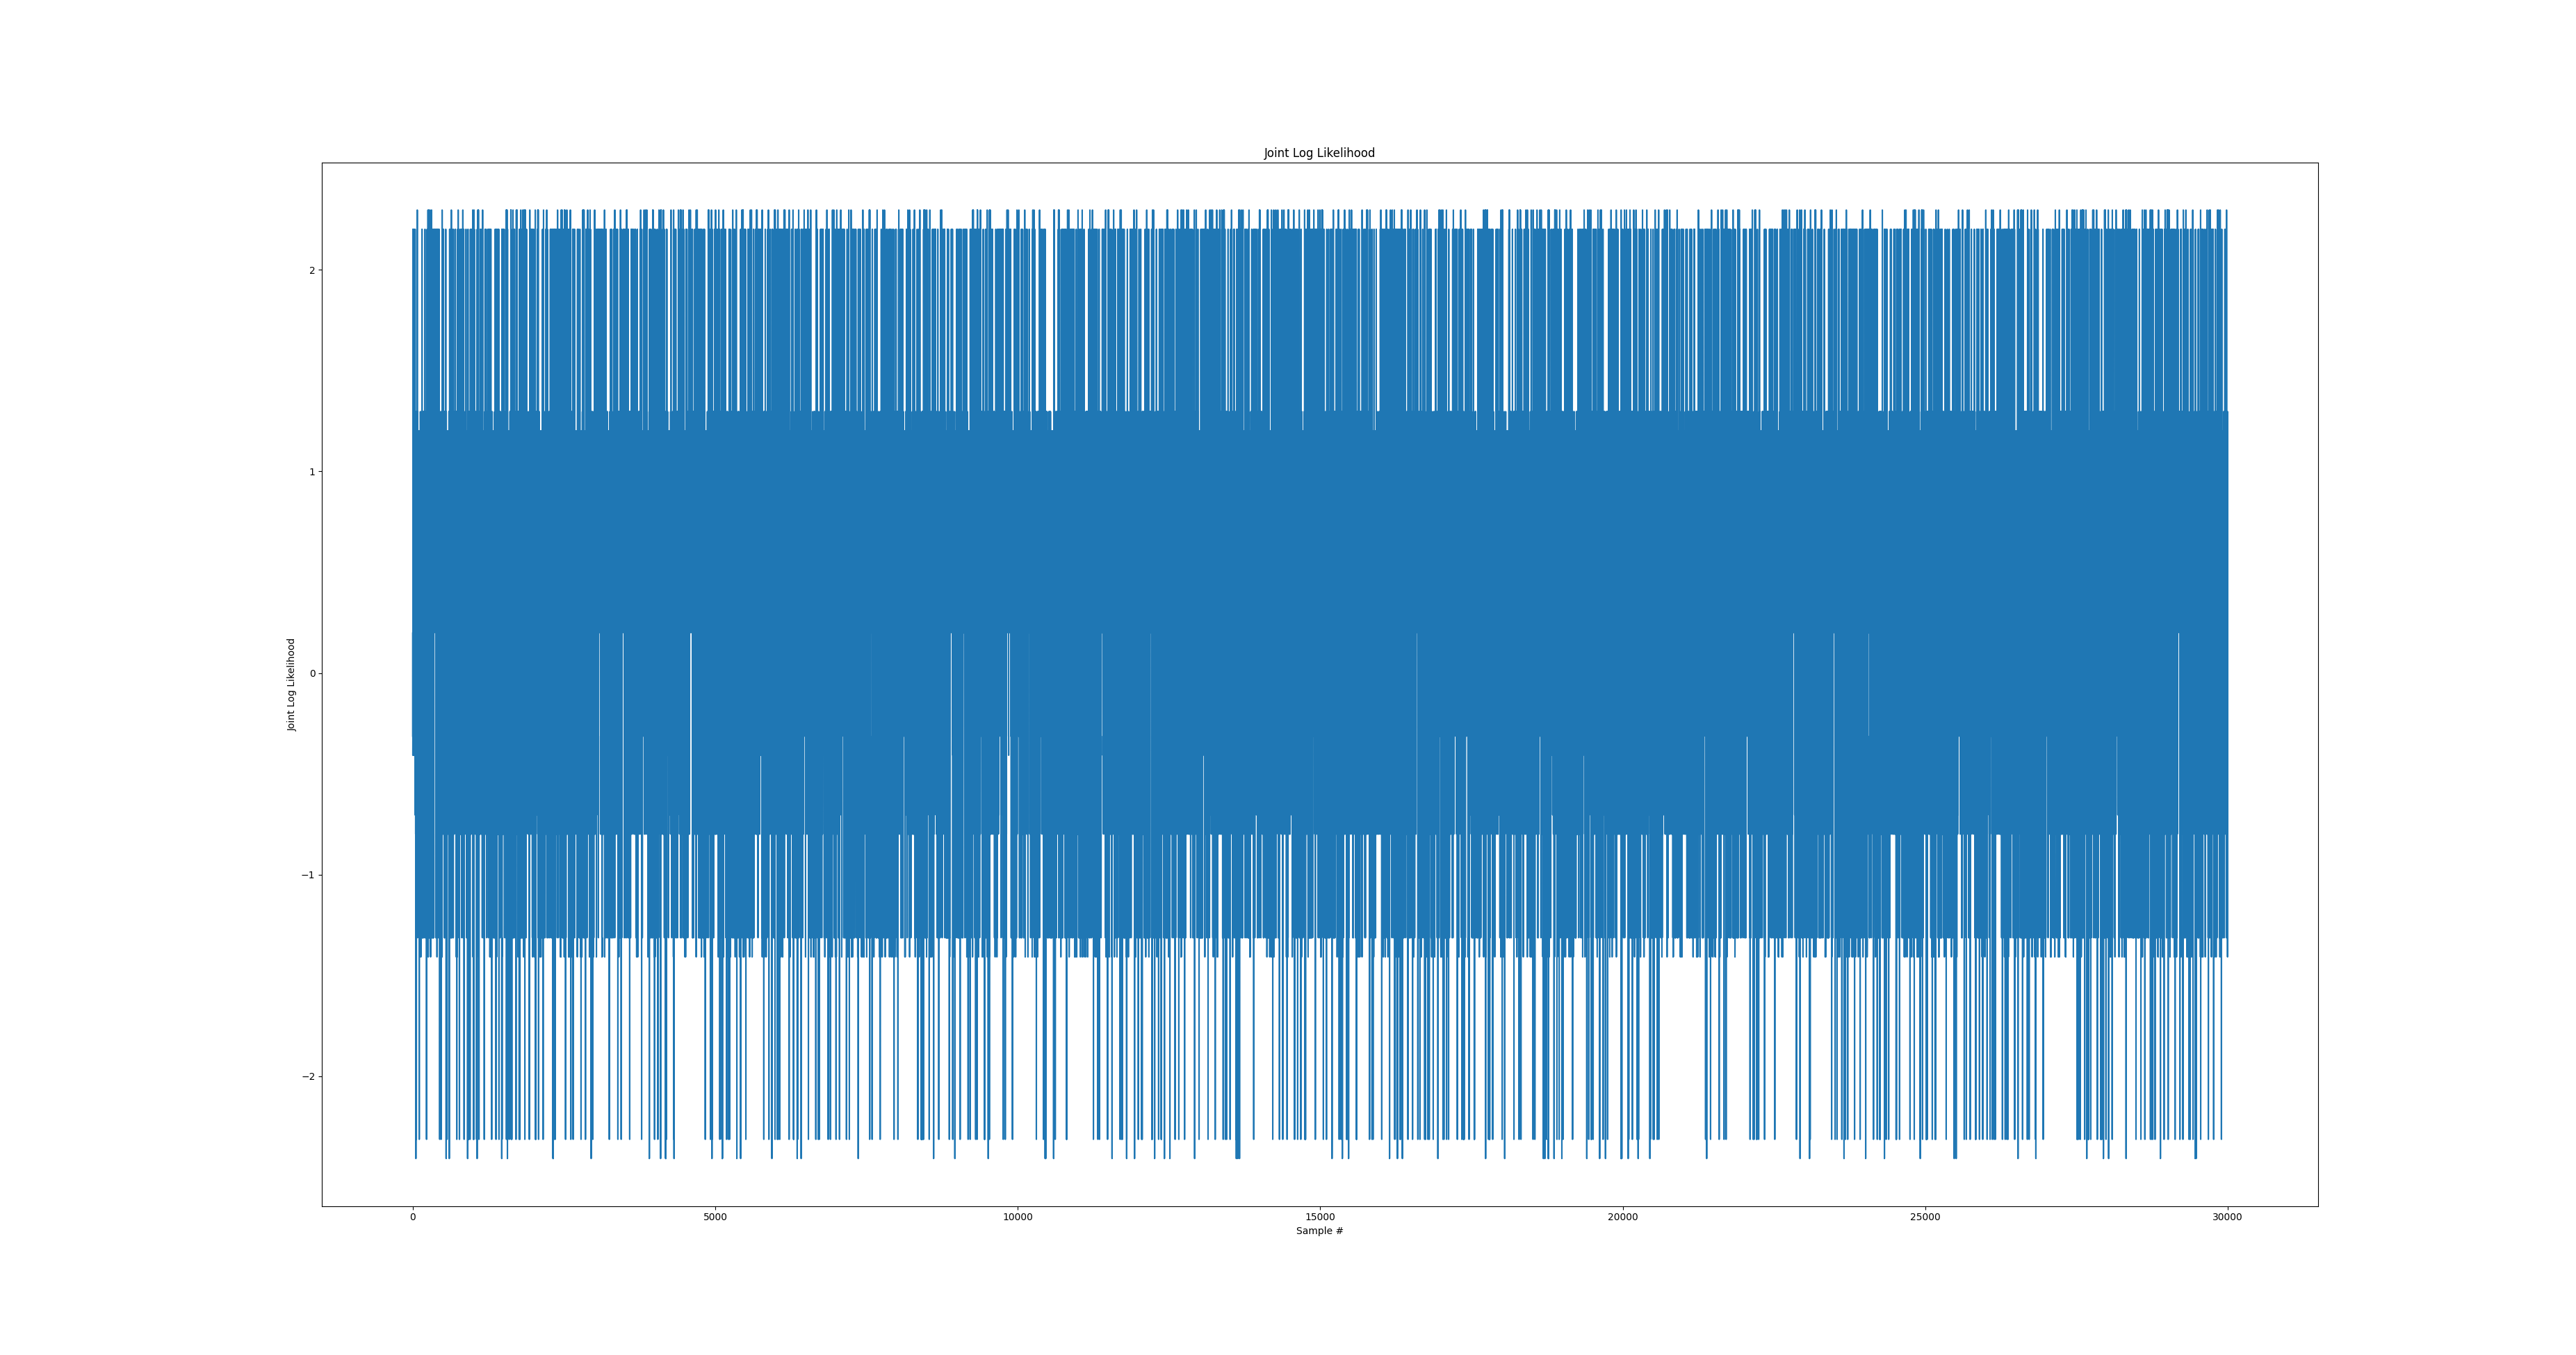
\includegraphics[width=\linewidth]{Figures/p4_MHGibbsjll.png}
\end{center}
\subsection{Program 5}
\begin{verbatim}
Collect samples denoted by program 5:
Elapsed time for program  5 .daphne is:  0:01:24.723336  seconds
tensor([[ 24.5000, -11.5213],
[ 13.6642,  -9.7524],
[ 13.6642,  -9.7524],
...,
[ 12.6109,  -5.6384],
[ 12.6109,  -5.6384],
[ 12.6109,  -5.6384]])
Mean of trace:  tensor([12.7786, -5.7767])  
and variance of trace:  tensor([0.1091, 0.1085])
\end{verbatim}
\begin{center}
	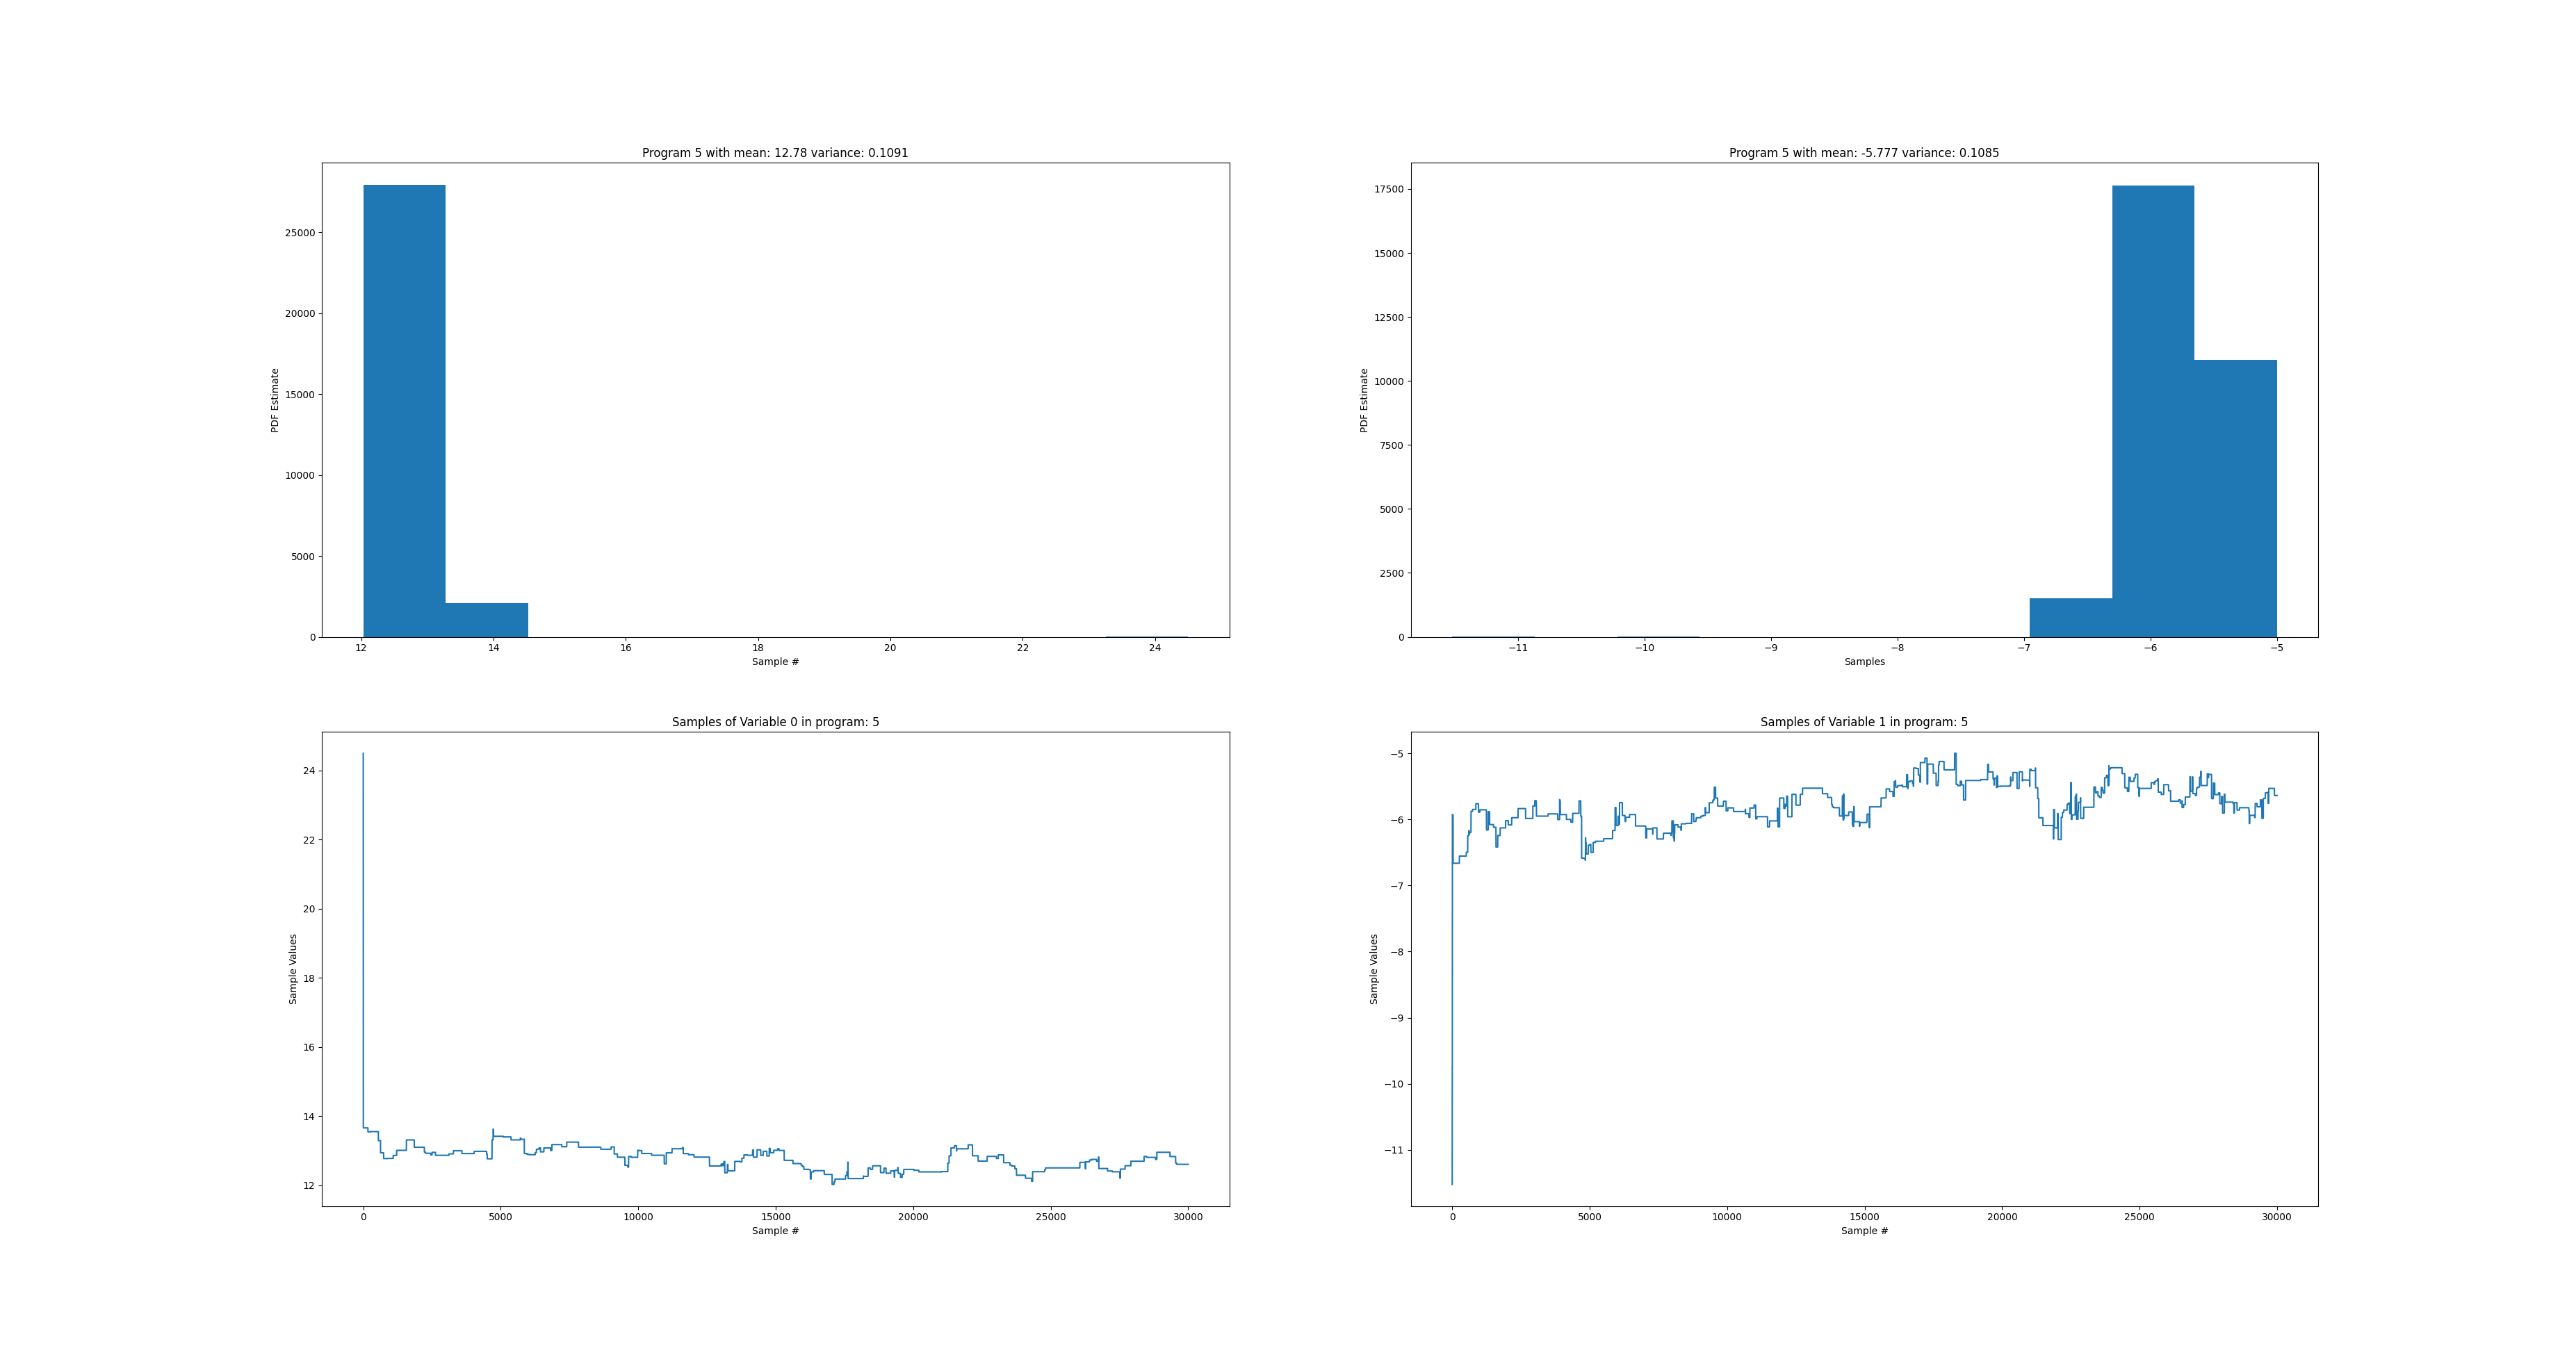
\includegraphics[width=\linewidth]{Figures/p5_MHGibbs.png}
\end{center}
\begin{center}
	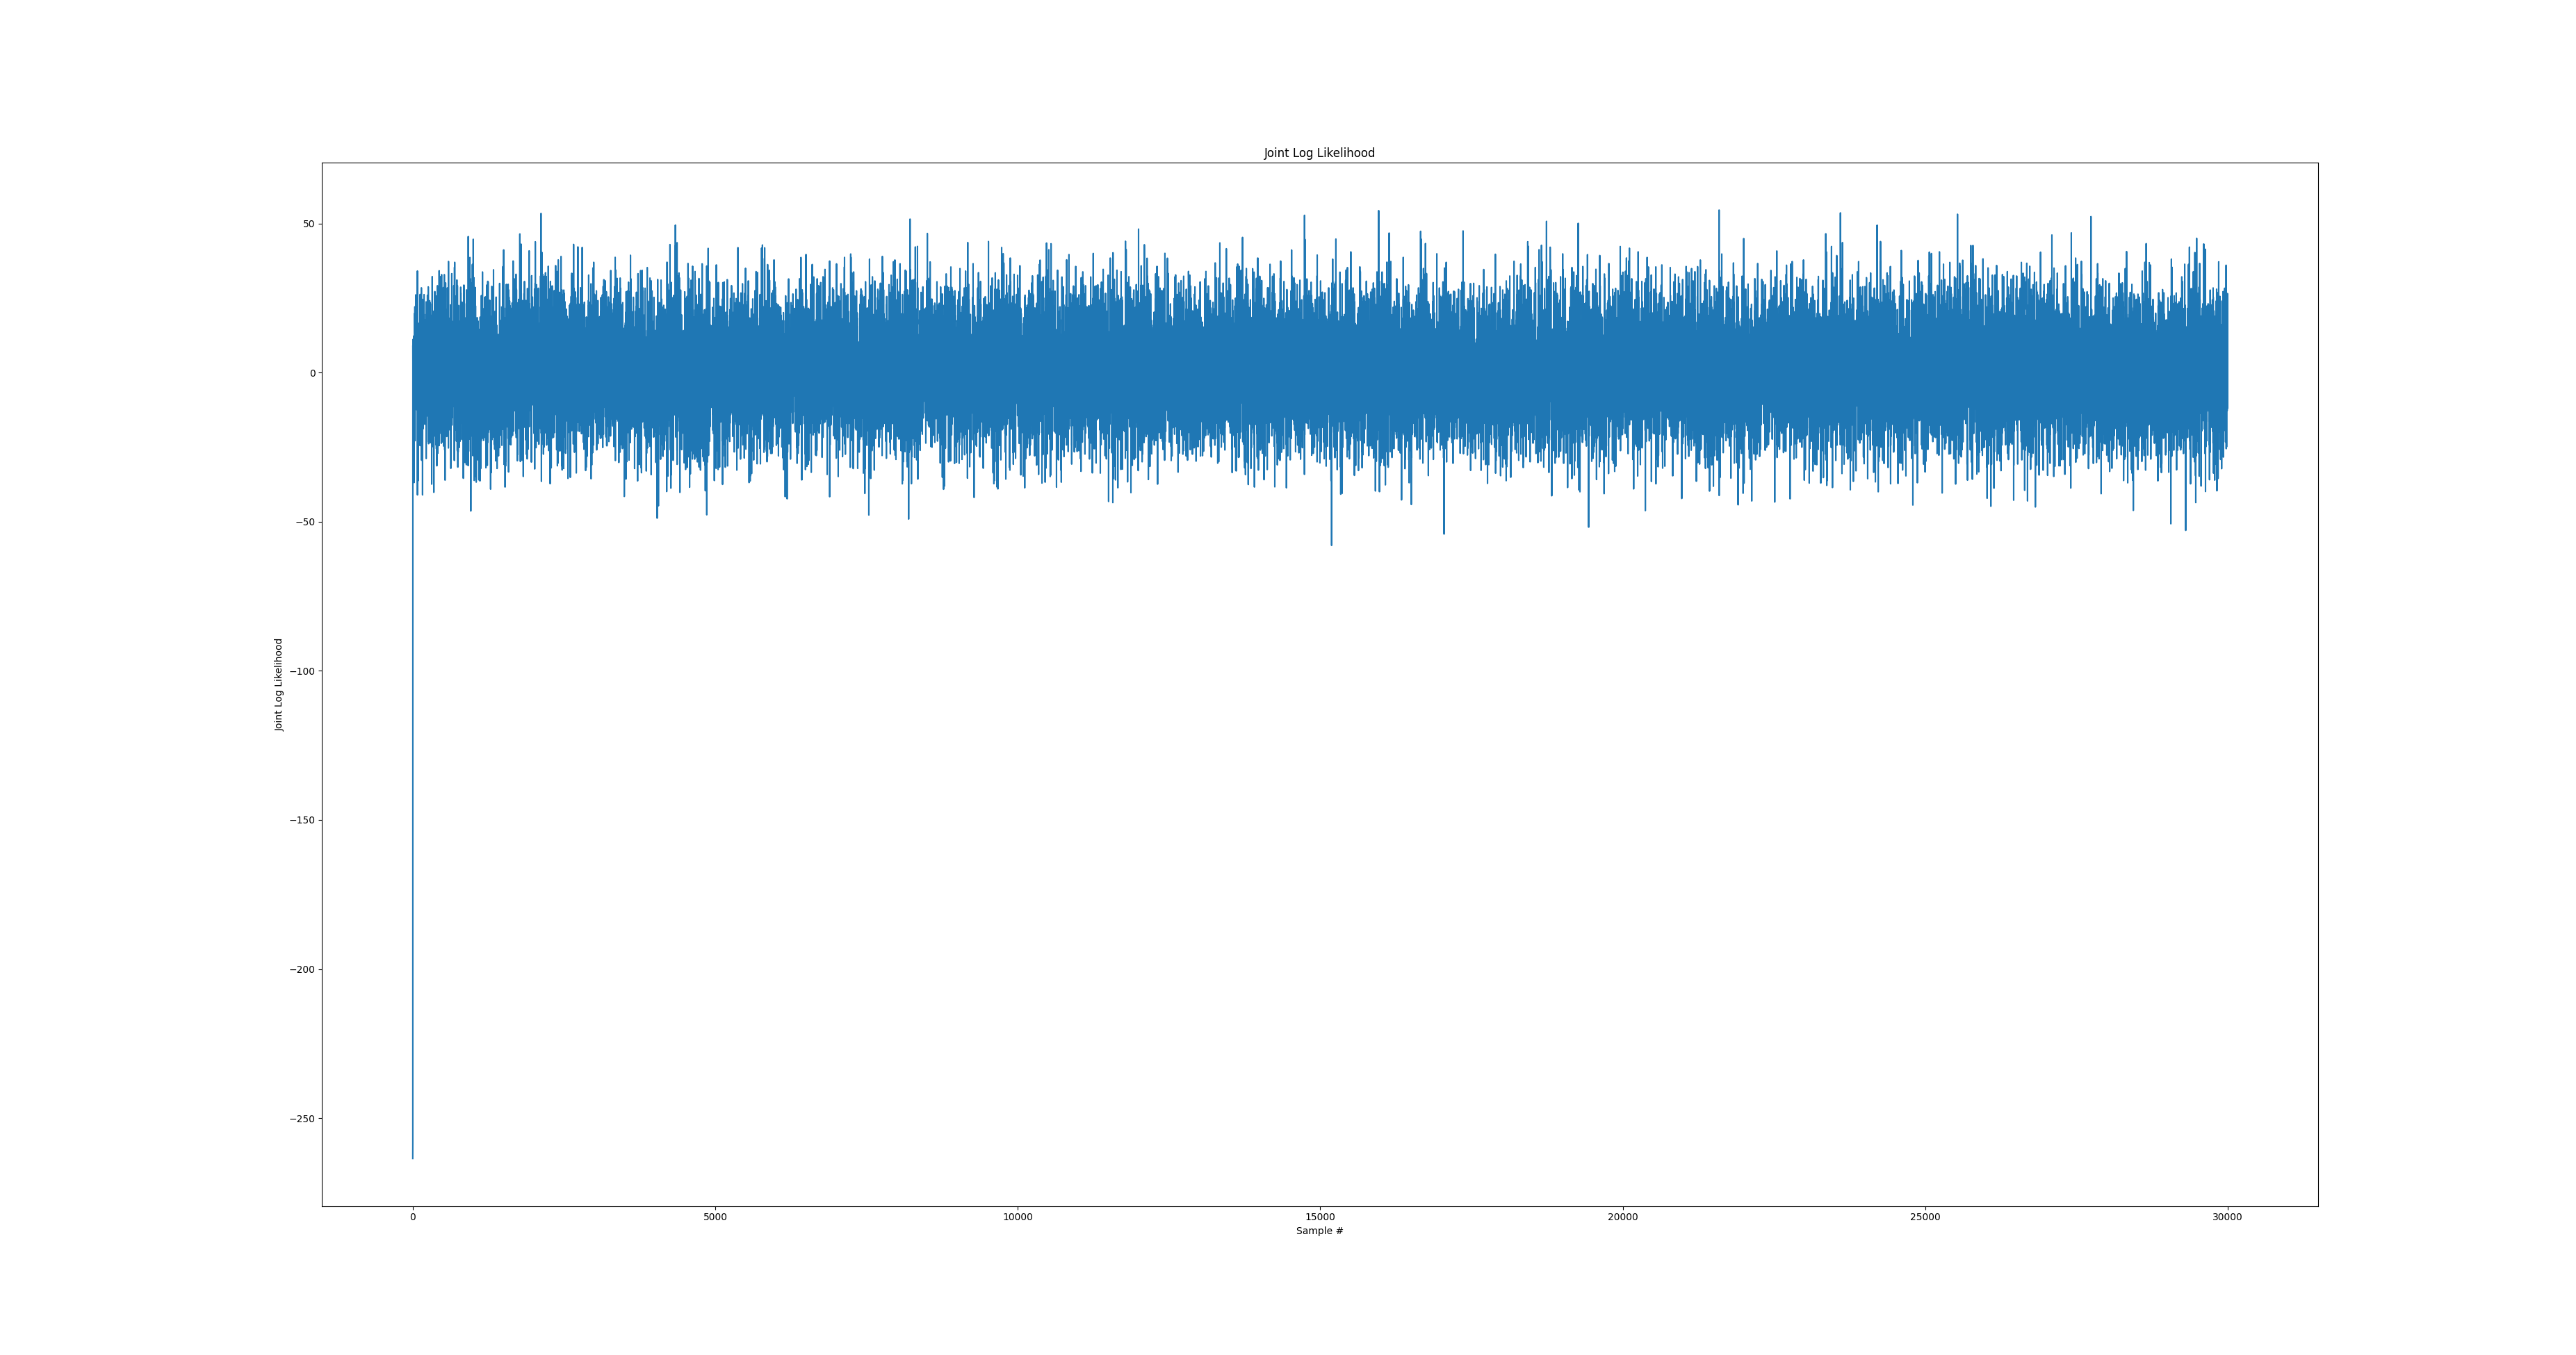
\includegraphics[width=\linewidth]{Figures/p5_MHGibbsjll.png}
\end{center}
\section{Hamoltanian Monte Carlo - HMC}
The HMC algorithm implements algorithms 18 and 19 where Pytorch autodiff is used to compute $\nabla U$. Similarly to the MH within Gibbs, the unobserved variables (latent) are initialized sampled from their respective priors and the Leapfrog integration technique numerically integrates the Hamiltonian formulation which is used to computed the acceptance ratio for a proposed new assignment for $X$:
\lstinputlisting[language = Python,linerange = {89-97} ]{HMC.py}
The Leapfrog integration algorithm implemented with dictionaries (would like to turn into matrix-vector operations!) follows algorithm 19:
\lstinputlisting[language = Python,linerange = {30-51} ]{HMC.py}
Where $\nabla U$ is computed:
\lstinputlisting[language = Python,linerange = {14-28} ]{HMC.py}
It is important to detach the gradient information at the next iteration because we want the gradient at the current point, not the gradient of the current point and all previous points. Lastly the Hamiltonian is computed as:
\lstinputlisting[language = Python,linerange = {112-127} ]{HMC.py}

Picking the number of integration steps and the step size to take from the gradient required some trial and error. A step size that is too large results in poor acceptance and no convergence, however a step size too small results in requiring many more samples to converge or explore the space. Here 5k samples are collected with each integration taking $T=20$ steps, and a step size $\epsilon = 0.01$ works reasonably well.
\subsection{Program 1}
\begin{verbatim}
Collect samples denoted by program 1:
Elapsed time for program  1 .daphne is:  0:01:41.703409  seconds
tensor(7.1211)
tensor([3.0656, 2.6720, 2.6331,  ..., 5.7209, 5.7209, 5.6698])
Mean of trace:  tensor(7.1211)  
and variance of trace:  tensor(0.7150)
\end{verbatim}
\begin{center}
	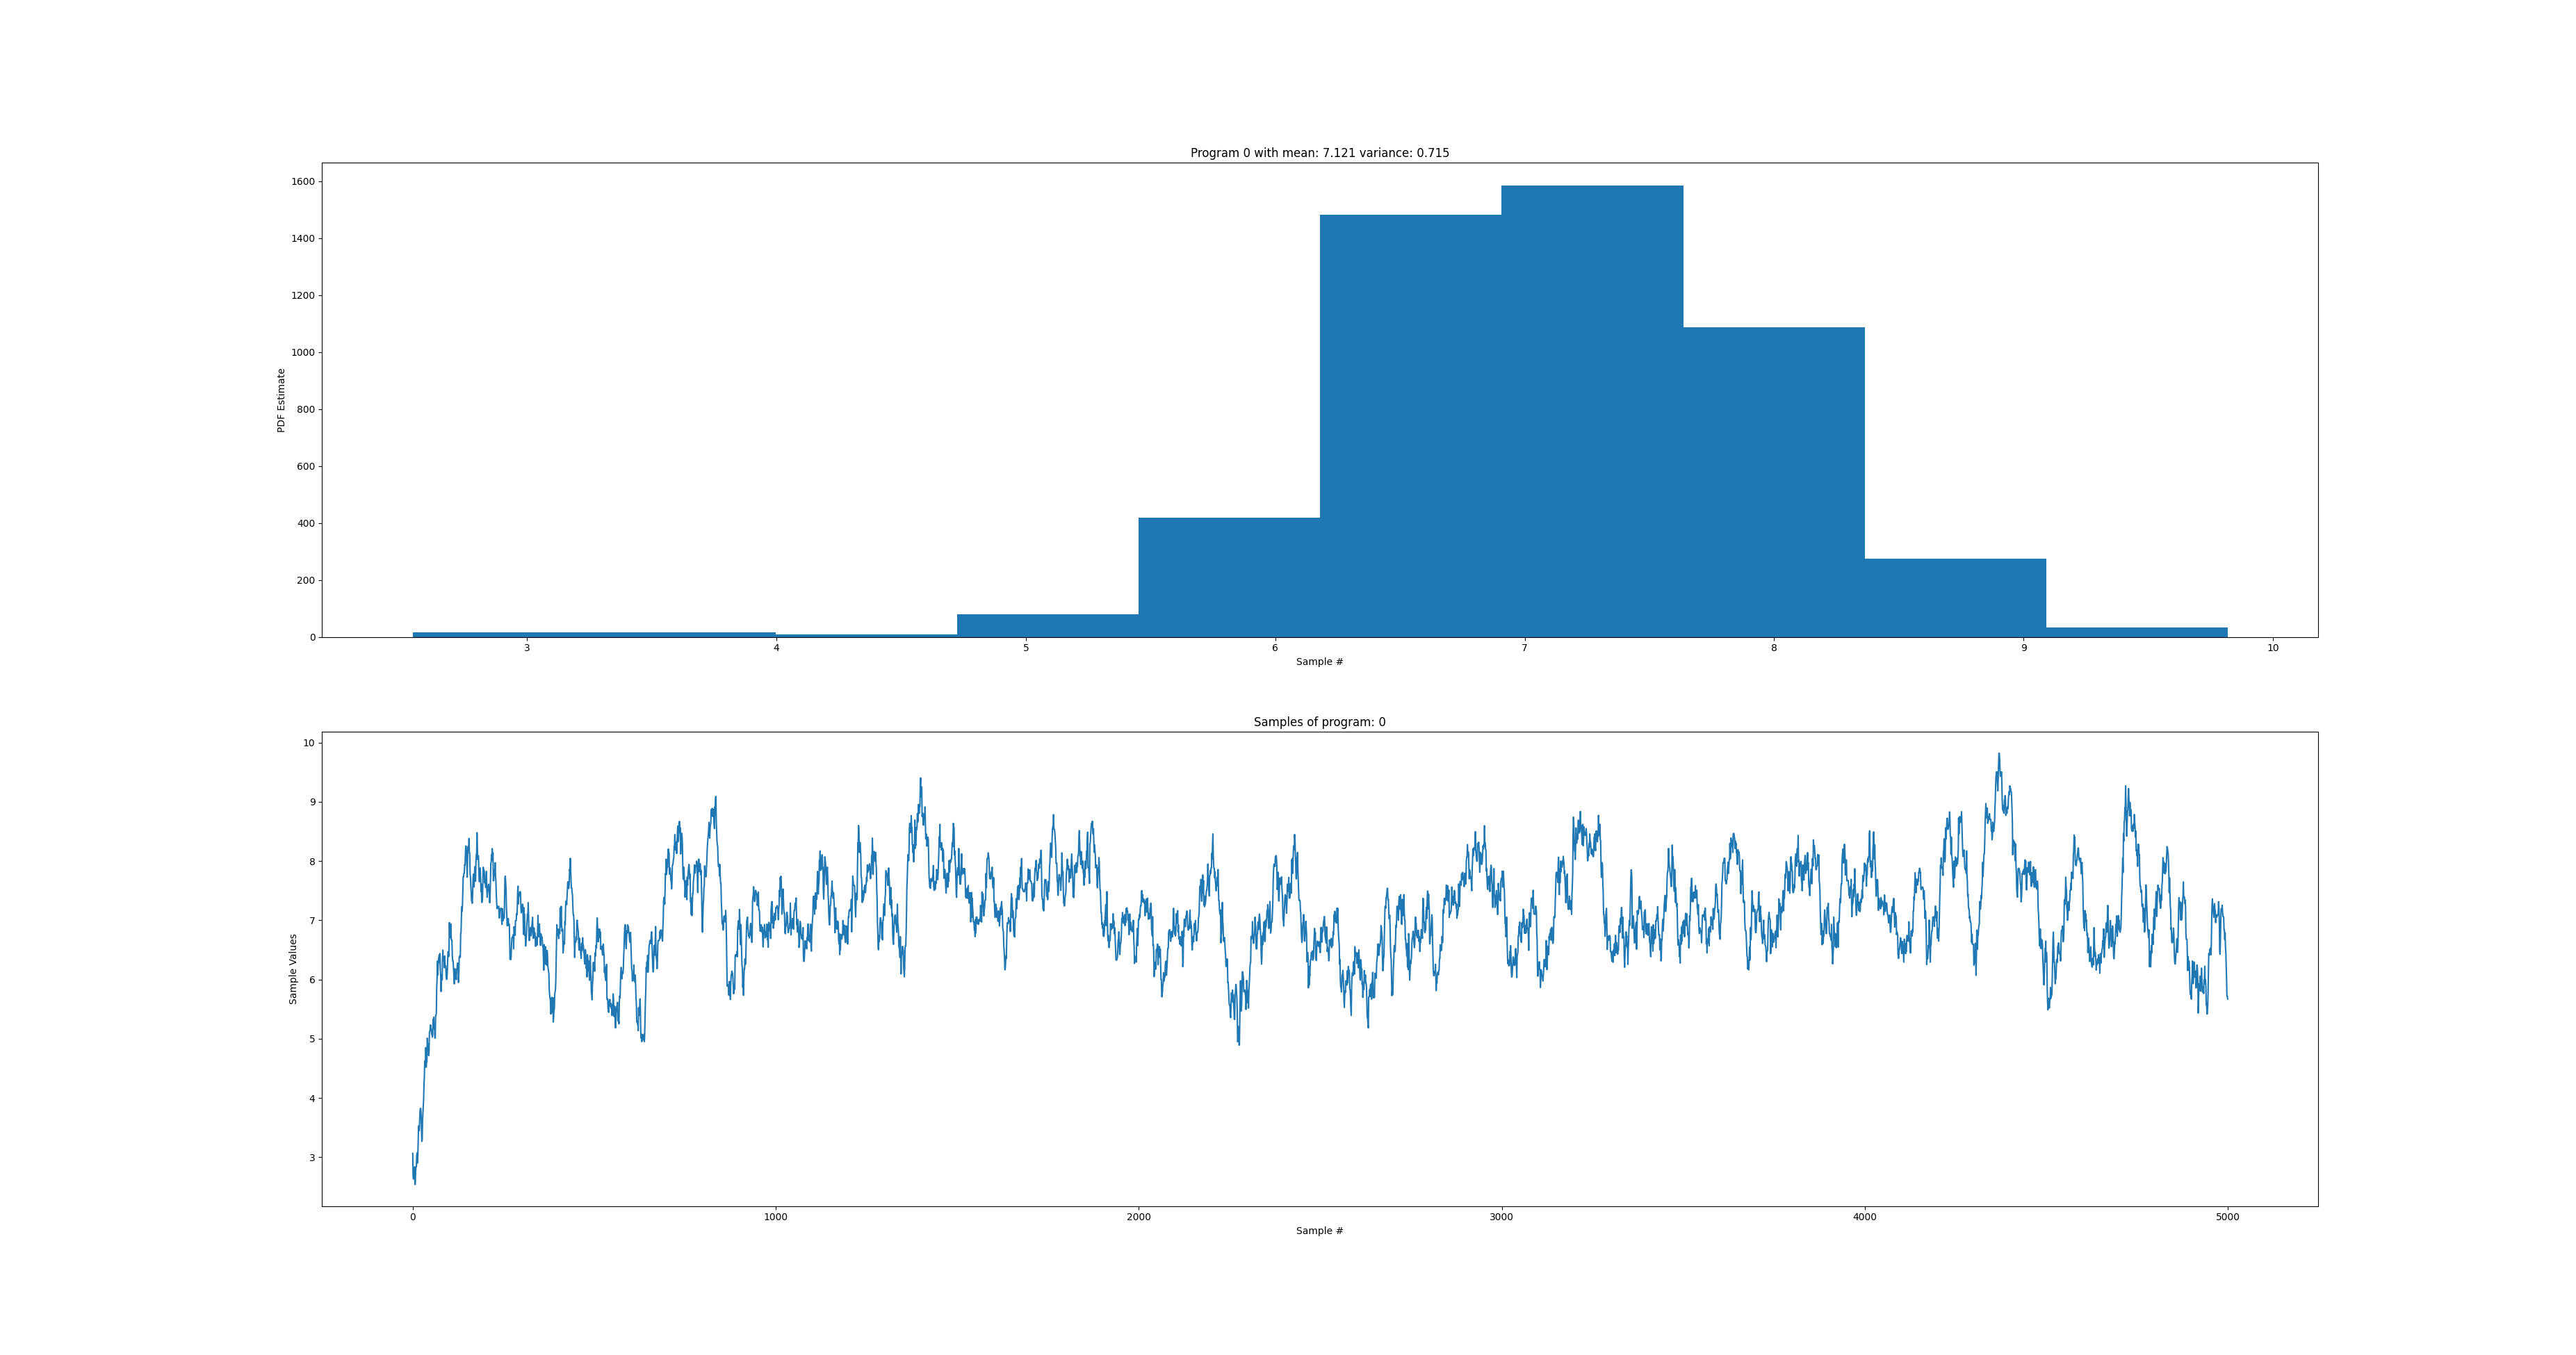
\includegraphics[width=\linewidth]{Figures/p1_HMC.png}
\end{center}
\begin{center}
	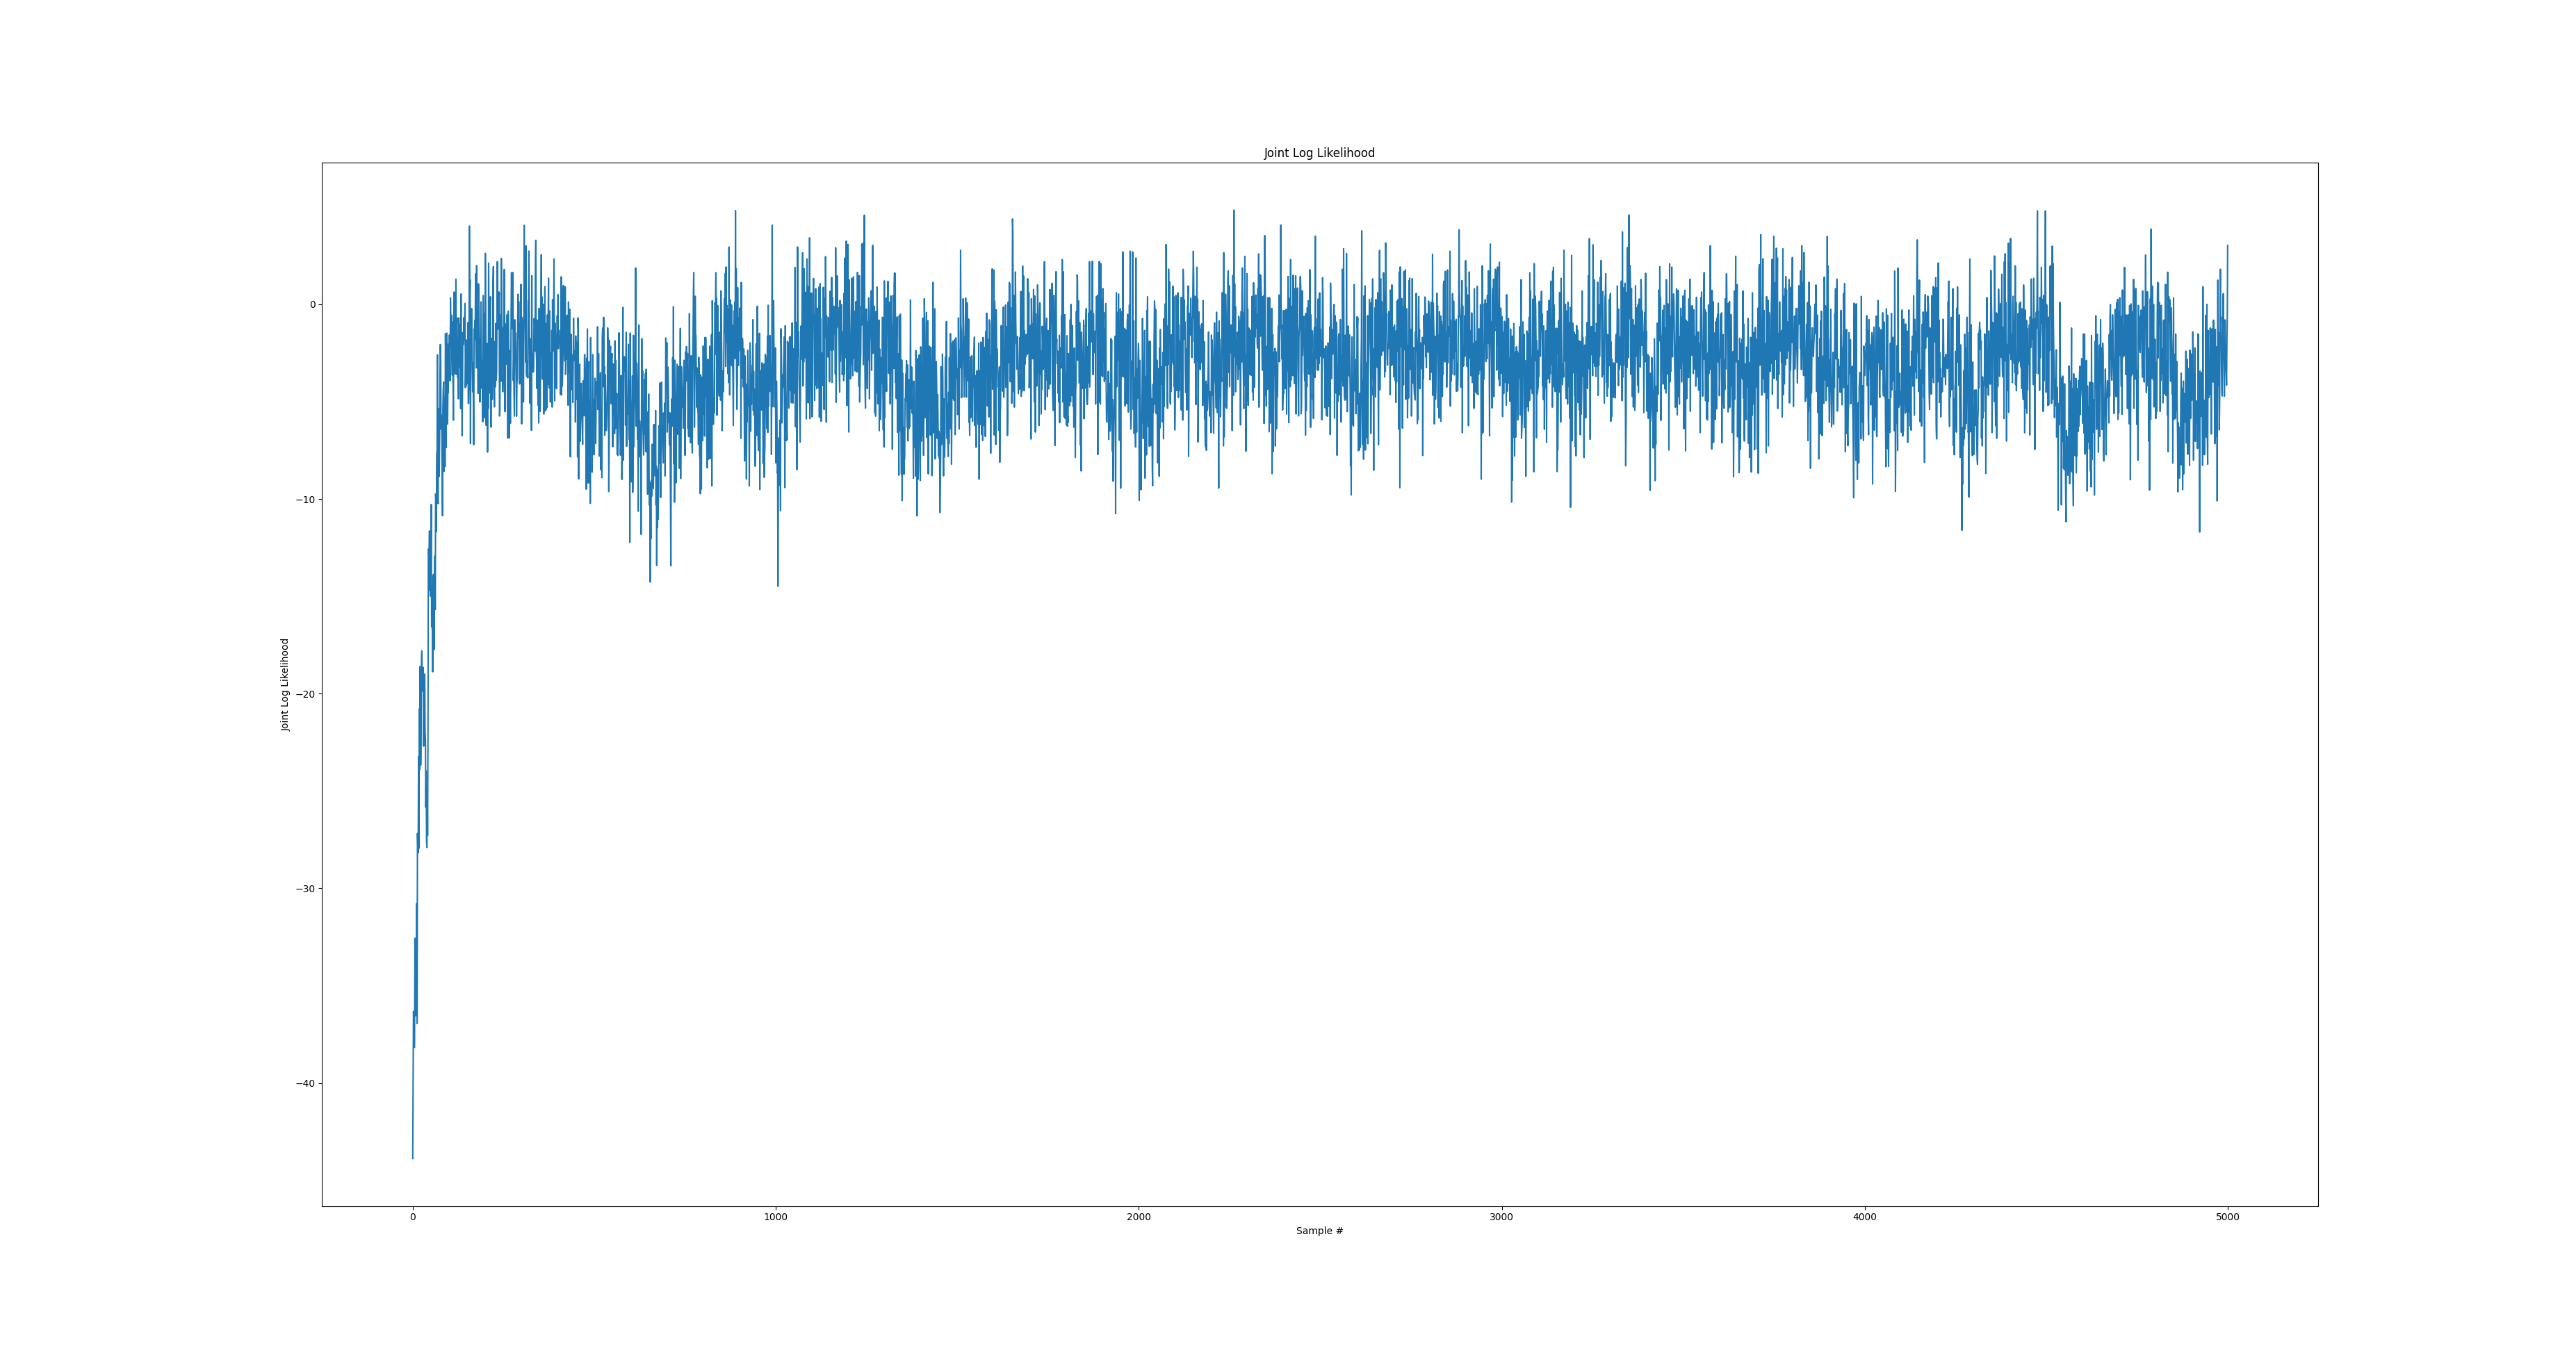
\includegraphics[width=\linewidth]{Figures/p1_HMCjll.png}
\end{center}
\subsection{Program 2}
\begin{verbatim}
Collect samples denoted by program 2:
Elapsed time for program  2 .daphne is:  0:04:12.794452  seconds
tensor([ 2.1201, -0.3792])
tensor([[ 6.3440, -1.0281],
[ 1.1802, -2.0720],
[ 2.8143, -1.7802],
...,
[ 2.2089, -0.4581],
[ 2.1194, -0.5892],
[ 2.0376, -0.5493]])
Mean of trace:  tensor([ 2.1201, -0.3792])  
and variance of trace:  tensor([0.0460, 0.5714])
The covariance matrix:  
[[ 0.04598997 -0.1326305 ]
[-0.1326305   0.57140268]]
\end{verbatim}
\begin{center}
	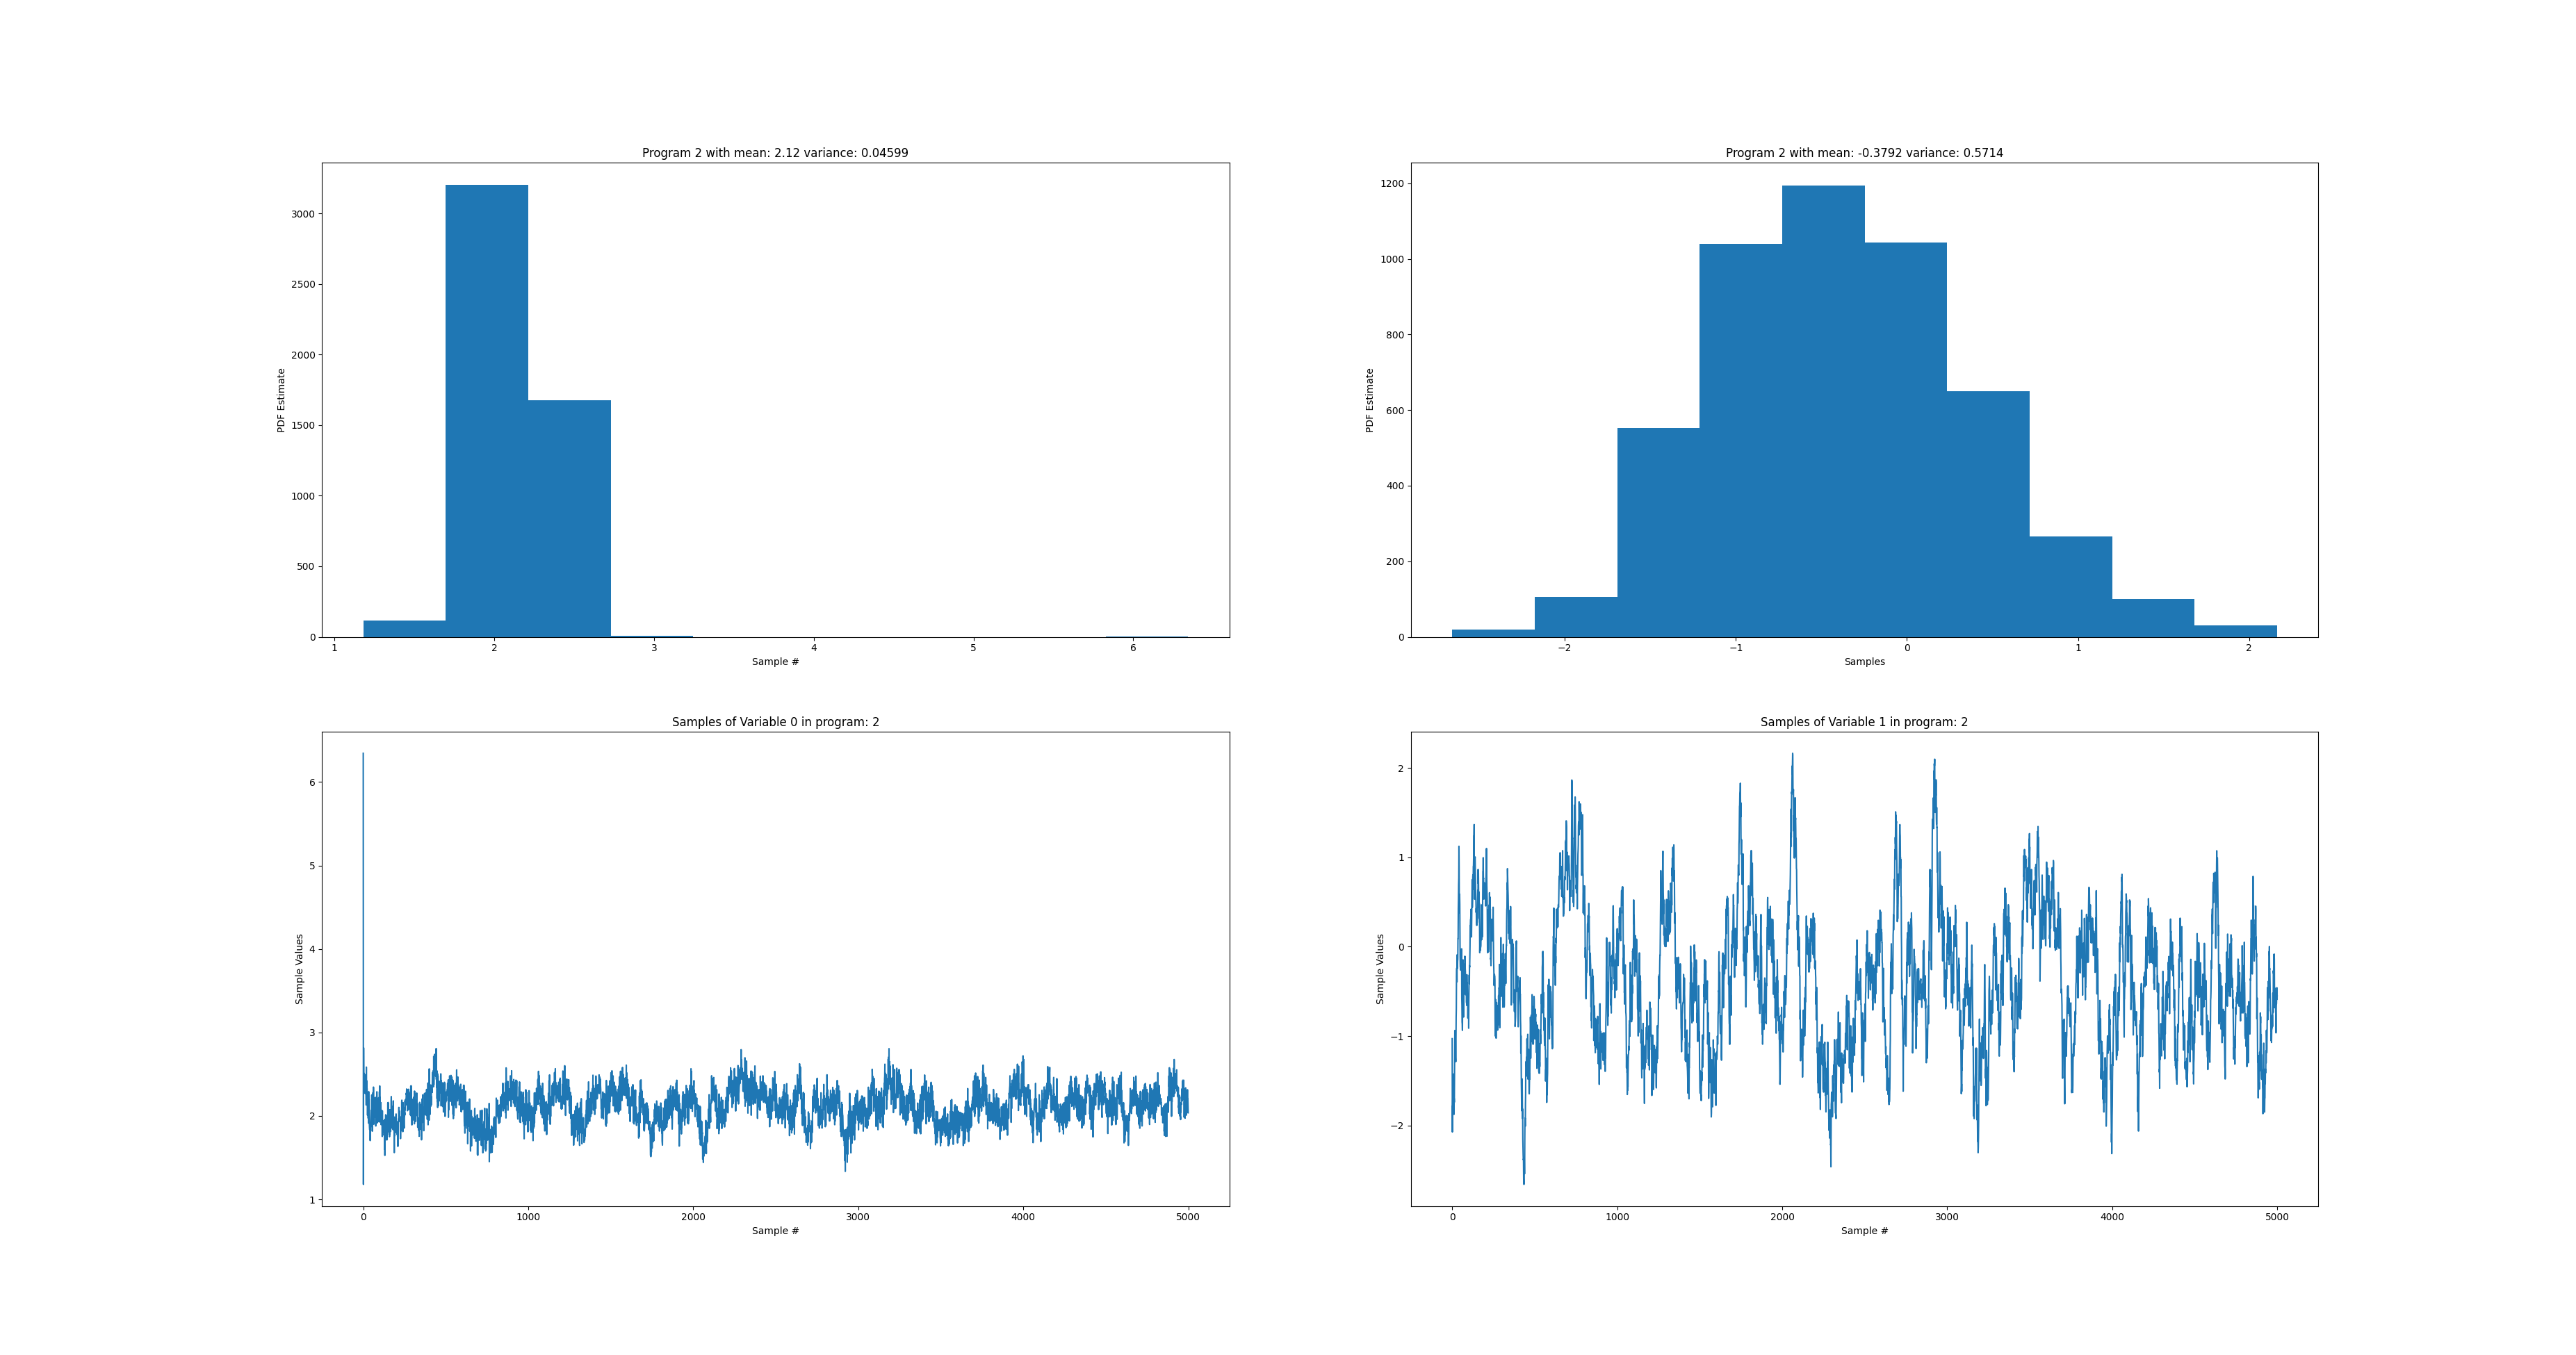
\includegraphics[width=\linewidth]{Figures/p2_HMC.png}
\end{center}
\begin{center}
	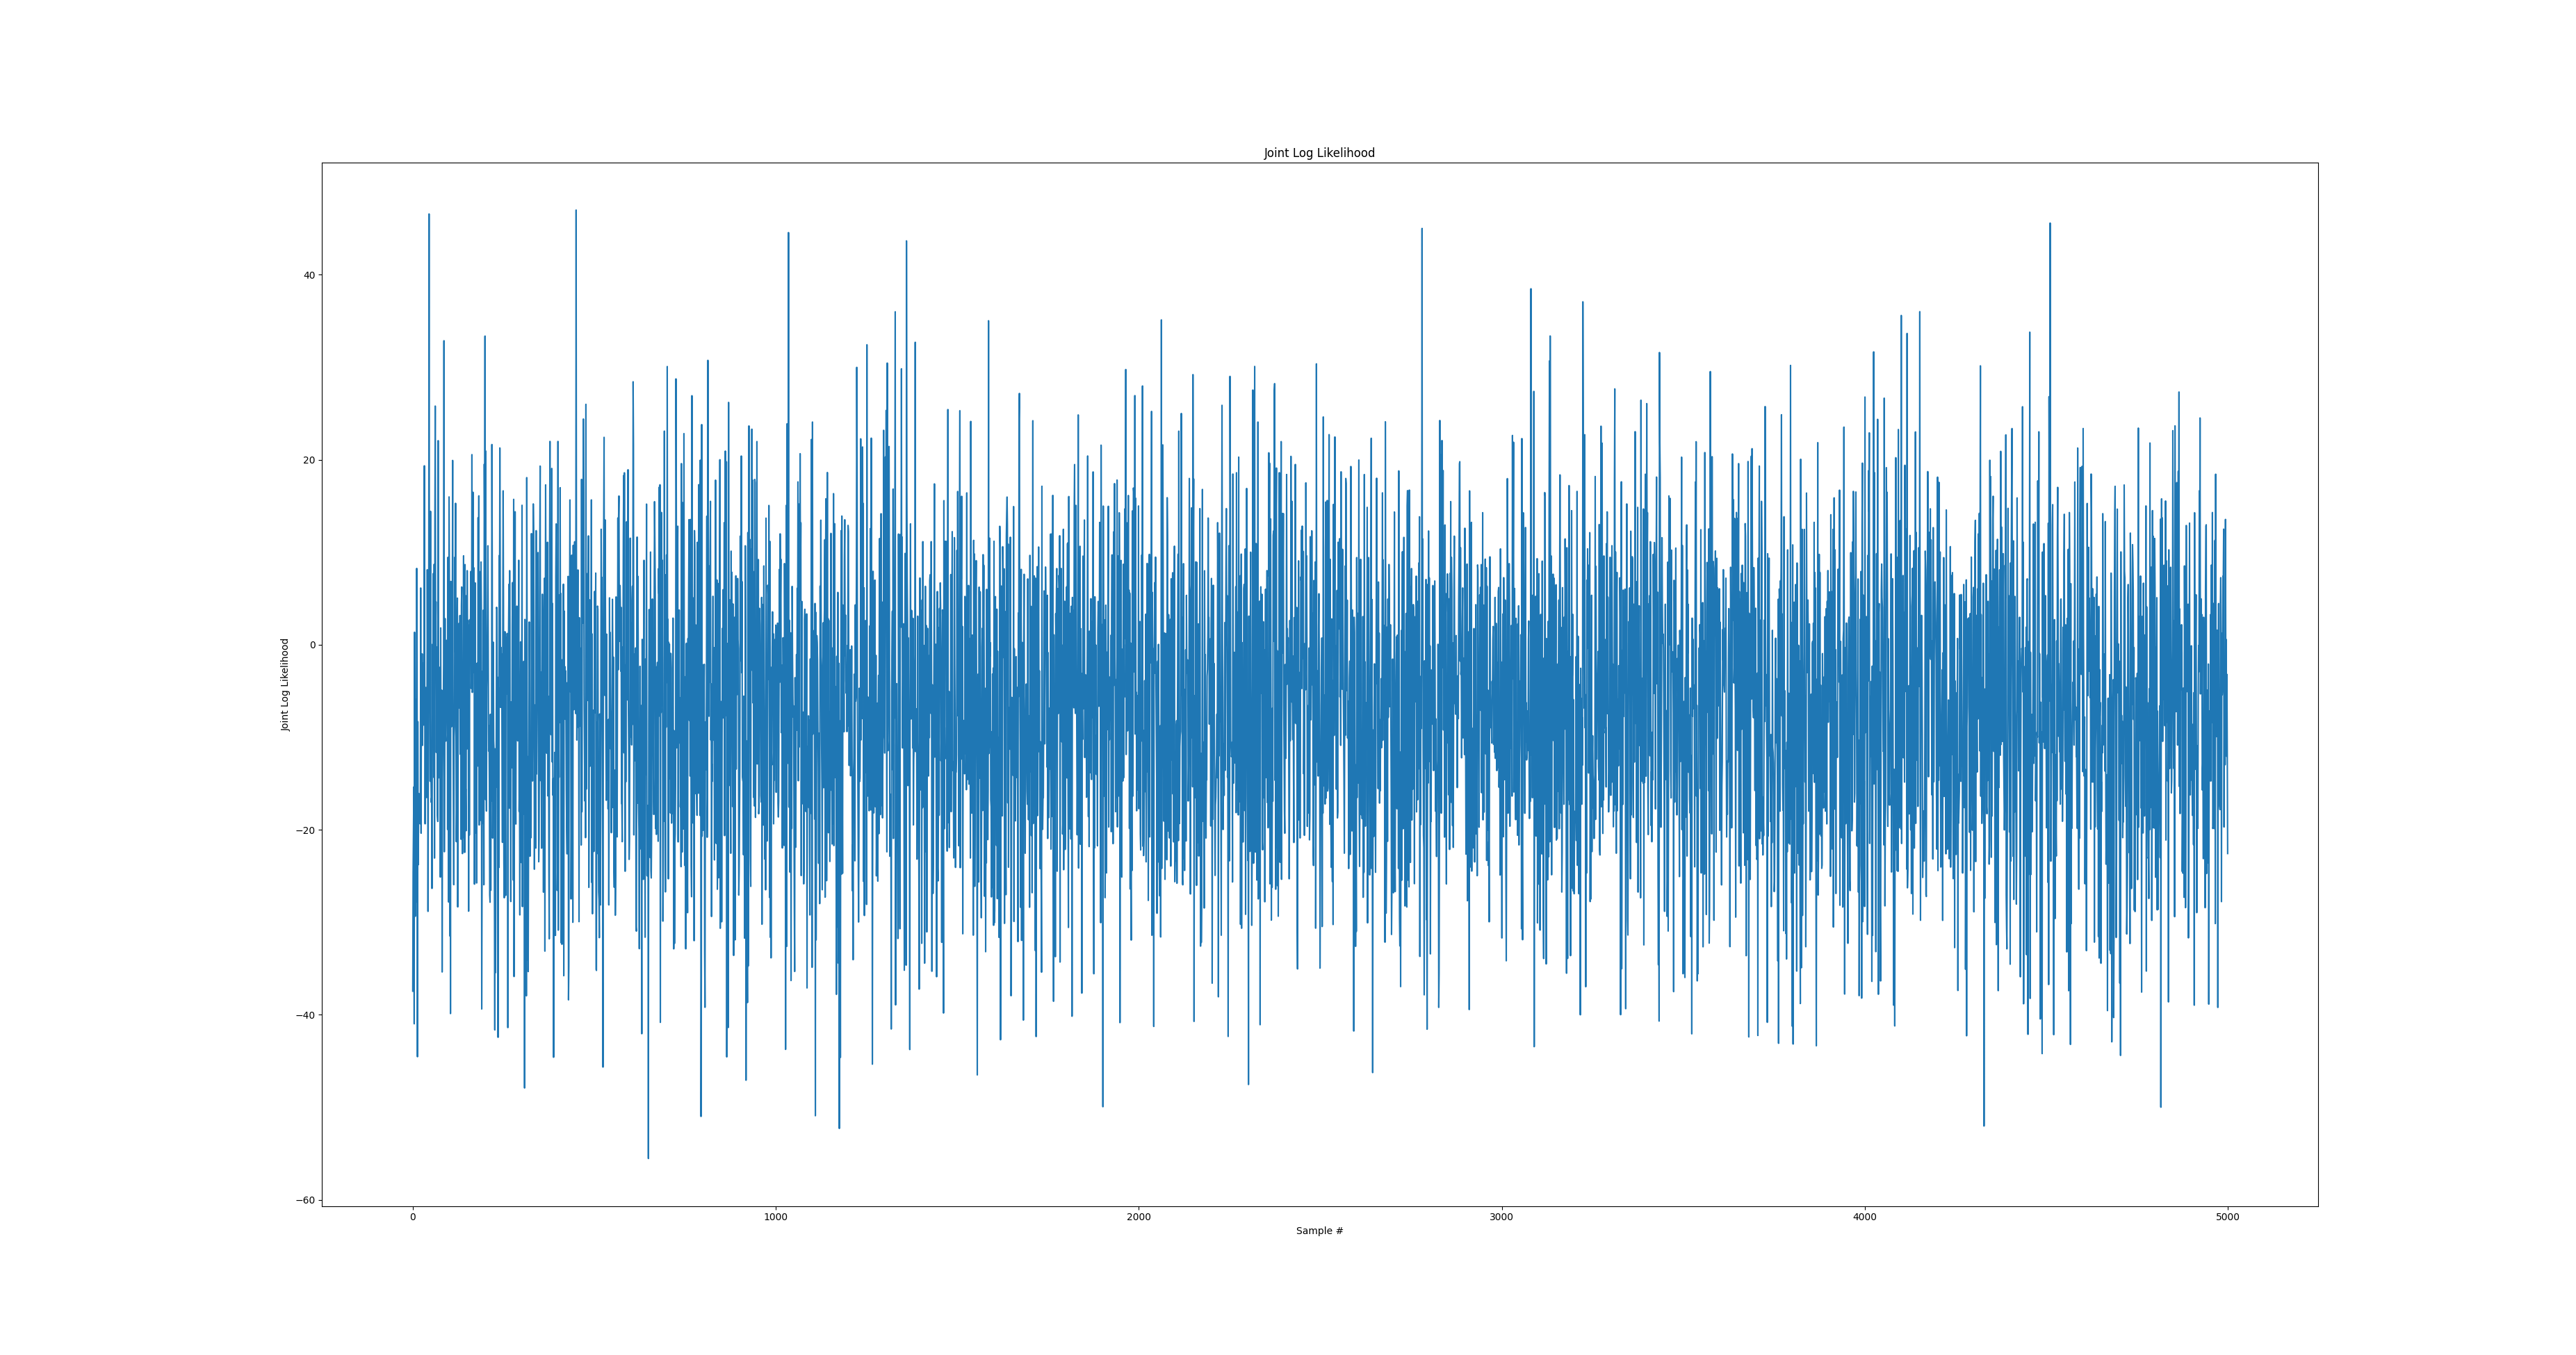
\includegraphics[width=\linewidth]{Figures/p2_HMCjll.png}
\end{center}
\subsection{Program 5}
For program 5, I had to change the step size parameters $\epsilon$ from $0.1$ to $0.01$ otherwise HMC fails. This allows the system to be kicked harder. However notice that when it snaps into the Dirac distributed area it stays there.
\begin{verbatim}
Collect samples denoted by program 5:
Elapsed time for program  5 .daphne is:  0:01:34.285442  seconds
tensor([-2.4993,  9.3750])
tensor([[-1.2606,  8.4221],
[ 0.1093,  6.8895],
[ 0.1093,  6.8895],
...,
[-2.5023,  9.3779],
[-2.5023,  9.3779],
[-2.5023,  9.3779]])
Mean of trace:  tensor([-2.4993,  9.3750])  
and variance of trace:  tensor([0.0080, 0.0075])
\end{verbatim}
\begin{center}
	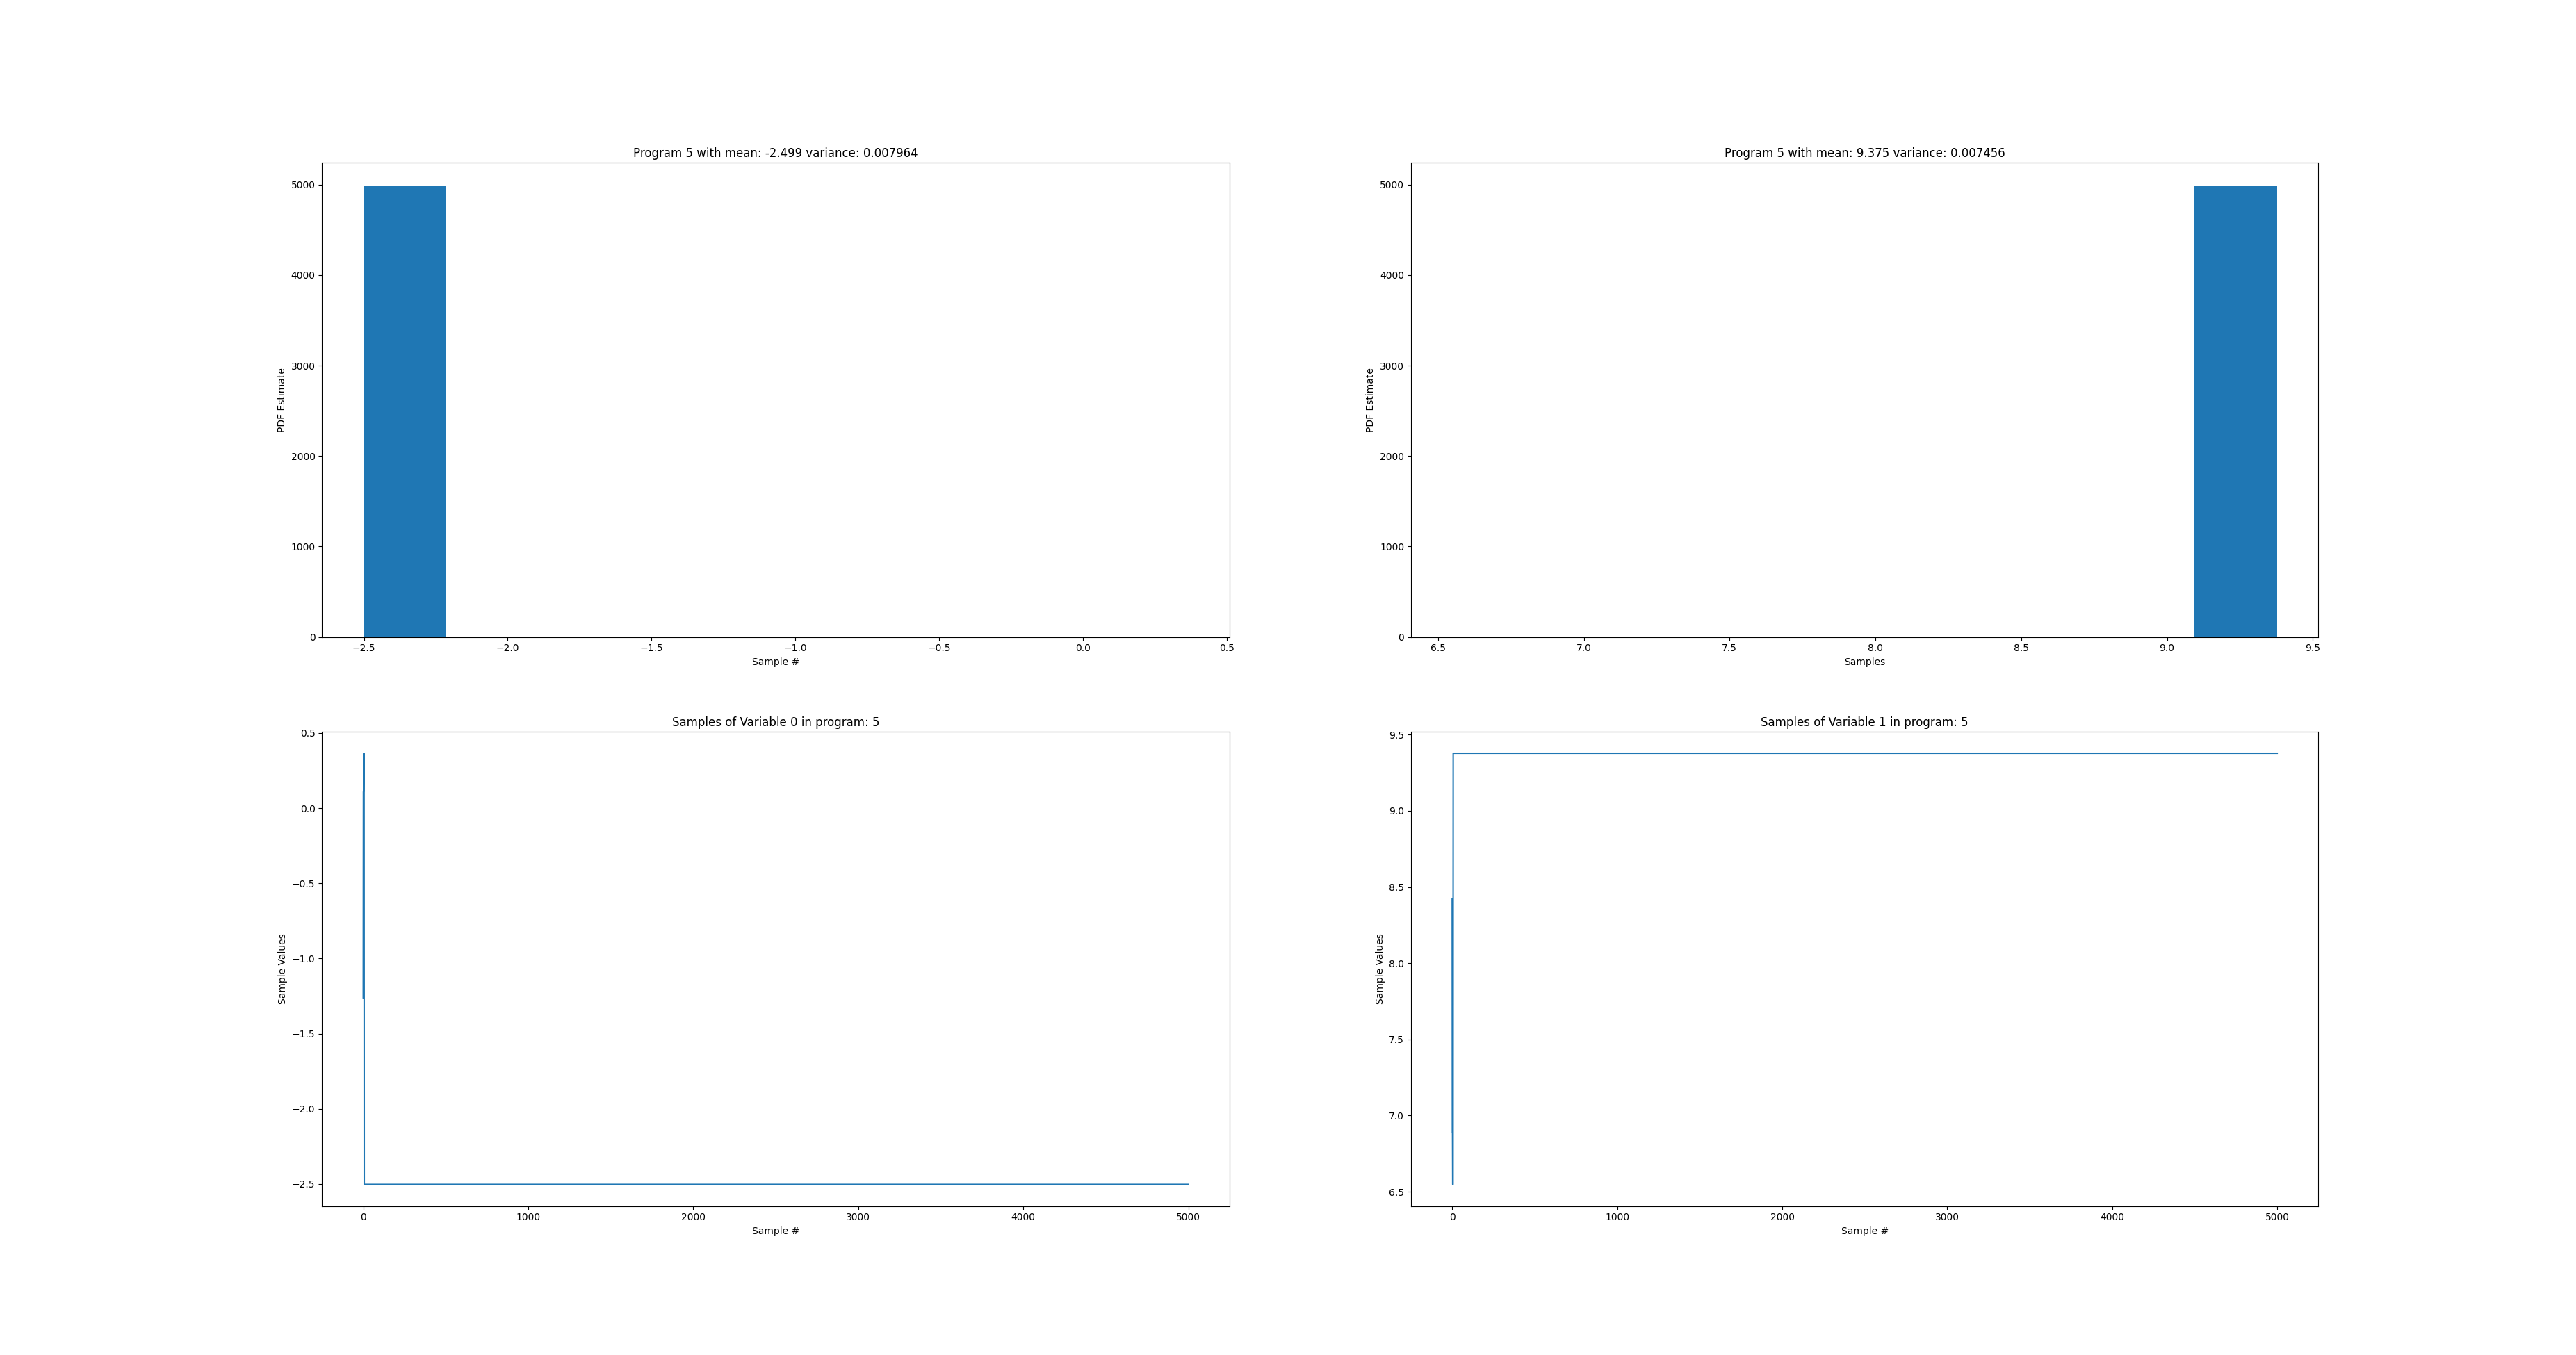
\includegraphics[width=\linewidth]{Figures/p5_HMC.png}
\end{center}
\begin{center}
	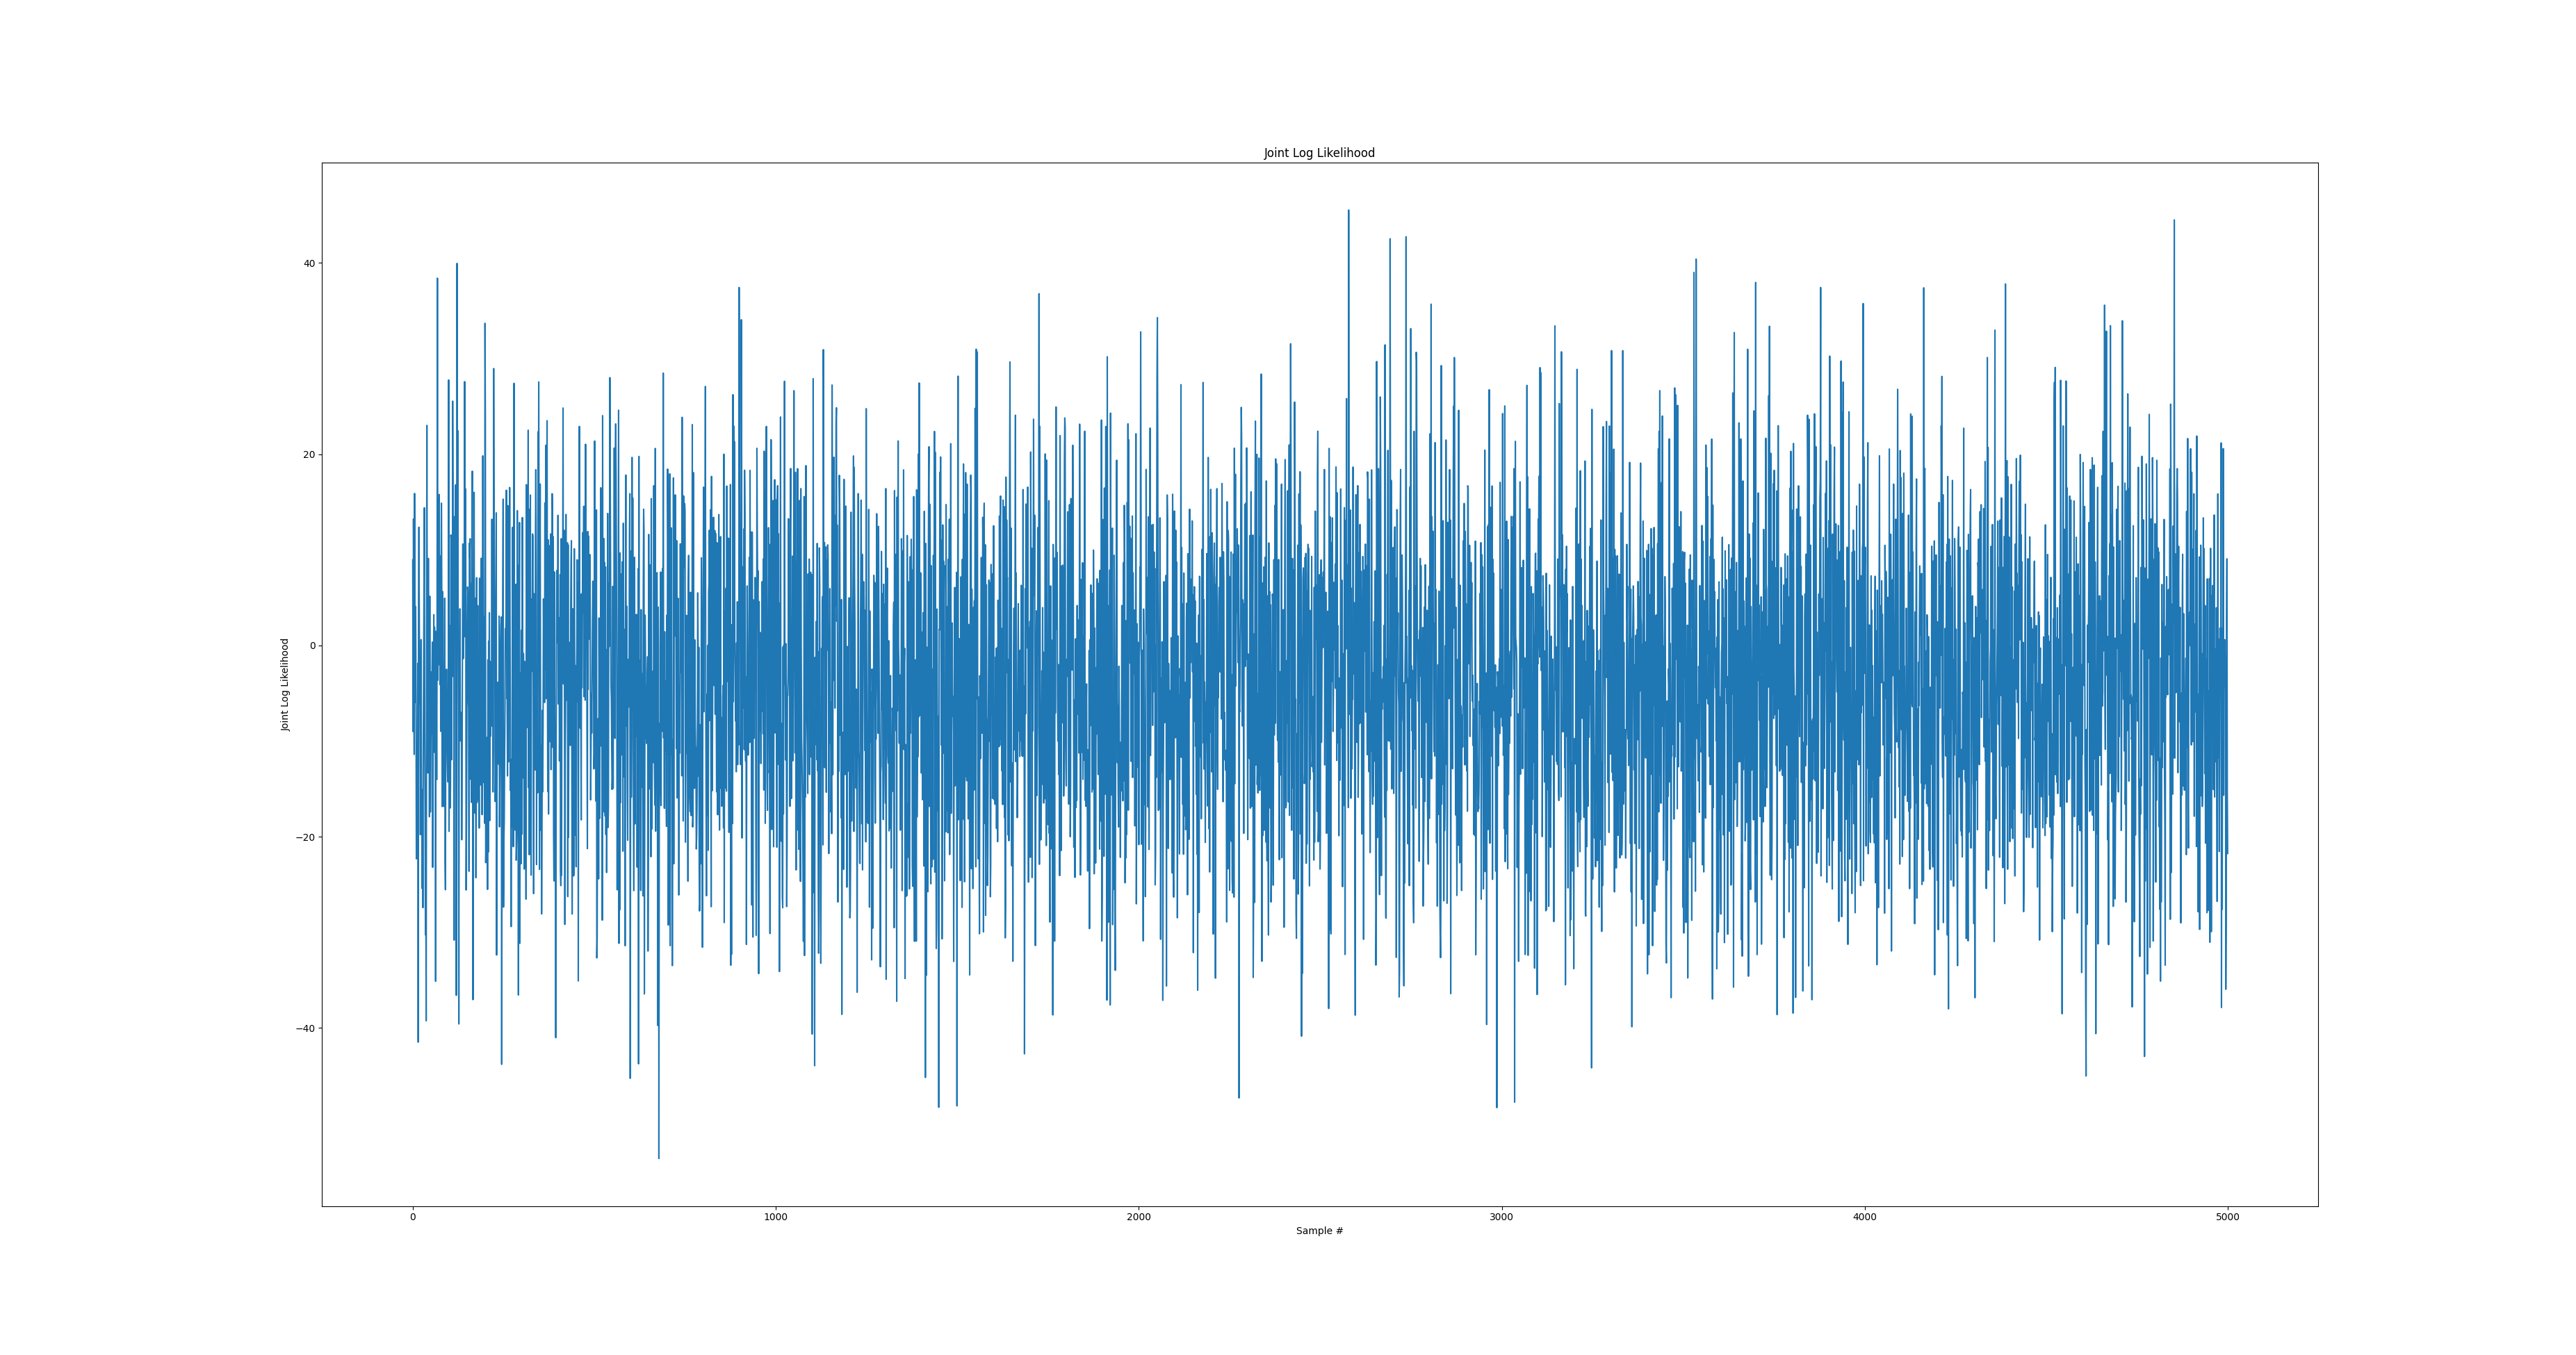
\includegraphics[width=\linewidth]{Figures/p5_HMCjll.png}
\end{center}
\end{document}
